\documentclass{beamer}[10]
\usepackage[portuguese]{babel}
\usepackage{pgf}
\usepackage[utf8]{inputenc}
\usepackage{beamerthemesplit}
\usepackage{graphics,epsfig, subfigure}
\usepackage{url}
\usepackage{srcltx}
\usepackage{hyperref}
\usepackage{ragged2e}
\usepackage{cancel} % para poder colocar o tracinho de cancelamento
\usepackage{multicol}
\usepackage{sgame} % to make payoff matrixes
\usepackage{qtree} % to make tree diagrams


\graphicspath{{./images/}} % set an default images folder

\definecolor{kugreen}{RGB}{50,93,61}
\definecolor{kugreenlys}{RGB}{132,158,139}
\definecolor{kugreenlyslys}{RGB}{173,190,177}
\definecolor{kugreenlyslyslys}{RGB}{214,223,216}

\setbeamercovered{transparent}

\setbeamerfont{section in sidebar}{size=\fontsize{6}{6}\selectfont}
\setbeamerfont{subsection in sidebar}{size=\fontsize{6}{6}\selectfont}
\setbeamerfont{subsubsection in sidebar}{size=\fontsize{6}{6}\selectfont}

\mode<presentation>
\usetheme[numbers,totalnumber,compress,sidebarshades]{PaloAlto}
\setbeamertemplate{footline}[frame number]
\justifying

  \usecolortheme[named=kugreen]{structure}
  \useinnertheme{circles}
  \usefonttheme[onlymath]{serif}
  \setbeamercovered{transparent}
  \setbeamertemplate{blocks}[rounded][shadow=true]

\logo{
\includegraphics[width=1.55cm]{img00_UEA.png}}
%\useoutertheme{infolines} 

\title[Micro II]{Microeconomia II - 2021/02}
\author[2021/02]{Bruno de M. Ruas}
\institute{Escola Superior de Ciências Sociais\\Universidade do Estado do Amazonas}
\date{\today}

\begin{document}

% pagina de titulo
\frame{\titlepage \vspace{-0.5cm}} 

% Sumario
\frame{
\frametitle{Sumário}
\begin{multicols*}{2}
	\small
	\tableofcontents
	\normalsize
\end{multicols*}
}

%%%%%%%%%%%%%%%%%%%%%%%%%%%%%%%%%%%%%%%%%%%
\section{Apresentação}
%%%%%%%%%%%%%%%%%%%%%%%%%%%%%%%%%%%%%%%%%%%

\begin{frame}
	\Huge Introdução
\end{frame}

\begin{frame}
	\frametitle{Apresentação do Professor}
	Nome: Bruno de Melo Ruas
	\\~\\
	Formação:
	\begin{itemize}
		\item Graduação em Ciências Econômicas (UEA) em 2017
		\item Pós-graduação em Gestão Financeira (FGV) em 2020
		\item Cursando Análise e Desenvolvimento de Sistemas (PUC-MG)
	\end{itemize}

	Experiência:
	\begin{itemize}
		\item Monitorias de Intro. Eco, Macro I e Econometria
		\item Projeto Acadêmico de Iniciação Científica
		\item Observatório do Polo Industrial (UEA)
		\item Gerente de Orçamento da SEMSA-Manaus (2019-2020)
		\item Supervisor de Faturamento One Clinic (Atualmente)
	\end{itemize}
\end{frame}

\begin{frame}
	\frametitle{Ementa do Curso}
	\begin{itemize}
		\item Poder de Mercado;
		\item Monopólios e Monopsônios;
		\item Mercado de Fatores;
		\item Interação estratégica;
		\item Oligopólios: Equilíbrios de Cournot e Bertrand;
		\item Introdução à Teoria dos Jogos: Estratégias dominantes, Equilíbrio de Nash;
		\item Jogos dinâmicos, Jogos sequenciais;
		\item Introdução ao equilíbrio geral;
		\item Falhas de Mercados e ineficiência do equilíbrio;
		\item Externalidades;
		\item Bens Públicos;
		\item Assimetria de Informação.
	\end{itemize}
\end{frame}

\begin{frame}
	\frametitle{Bibliografia}
	\begin{itemize}
		\item Varian, Hal. Microeconomia: Uma Abordagem Moderna. 6 ed. Rio de Janeiro: Campus Elsevier, 2003. (Principal)
		\item Goolsbee, Levitt e Syverson. Microeconomia. 2 ed. São Paulo: Atlas, 2008.
		\item Pindyck, Robert S.; Rubinfeld, Daniel L. Microeconomia. 6 ed. São Paulo: Pearson Prentice Hall, 2007.
		\item Bergstrom, Theodore C.; Varian, Hal R. Workouts in intermediate microeconomics. WW Norton, 2014.
		\item Varian, Hal R. Intermediate microeconomics with calculus: a modern approach. WW Norton \& Company, 2014.
	\end{itemize}
\end{frame}

\begin{frame}
	\frametitle{Metodologia}
	
	Professor:
	\begin{itemize}
		\item Aulas expositivas e dinâmicas (EAD ou presenciais) com os conteúdos propostos
		\item Material didático original elaborado específicamente para o curso (versão 1.0)
		\item Grupo no discord para tiragem de dúvidas e auxílios extra-classe
		\item Publicação de todo o material no repositório do Github
	\end{itemize}

	Alunos:
	\begin{itemize}
		\item Presença participativa em todas as aulas e, em caso de falta, esforço de recuperação do material perdido
		\item Leitura antecipada do material referente à cada aula prevista
		\item Realização dos exercícios propostos em sala de aula e para casa
	\end{itemize}

\end{frame}

\begin{frame}
	\frametitle{Panorama do Curso}

	Como o nome da disciplina deixa evidente, nós estamos continuando uma jornada que já se iniciou com a disciplina de Microeconomia I.
	\\~\\
	A essa altura, você deve ter o domínio de assuntos como:
	\begin{itemize}
		\item O Modelo de Escolha do Consumidor
		\begin{itemize}
			\item Restrição Orçamentária
			\item Curvas de Indiferença
			\item Excedente do Consumidor
		\end{itemize}
		\item A Oferta da Empresa competitiva
		\begin{itemize}
			\item Custos: Médio, Marginal, Total
			\item Curvas de isolucro
			\item Tecnologias de Produção 
		\end{itemize}
		\item Mercado de Fatores
		\item O Equilíbrio de Mercado competitivo
	\end{itemize}
\end{frame}

\begin{frame}
	\frametitle{Panorama do Curso}
	Os ferramentais usados ao longo do curso de microeconomia I também não devem ser nenhum mistério. Portanto, vocês já devem saber o que são:
	\\~\\
	\begin{itemize}
		\item Funções, funções Inversas, funções lineares, coeficientes angular e linear
		\item Variações e Taxas de Variação
		\item Derivadas e Derivadas Parciais
		\item Otimização e Otimização com Restrição
	\end{itemize}
	Então podemos seguir de onde micro I parou, né?
\end{frame}

\begin{frame}
	\frametitle{Panorama do Curso}
	\begin{center}
		
\includegraphics[scale=0.4]{img01.jpg}
	\end{center}
\end{frame}

%%%%%%%%%%%%%%%%%%%%%%%%%%%%%%%%%%%%%%%%%%%
\section{Preparativos}
%%%%%%%%%%%%%%%%%%%%%%%%%%%%%%%%%%%%%%%%%%%

\begin{frame}
	\Huge Preparativos
\end{frame}

\begin{frame}
	\frametitle{Funções}
	Vamos relembrar as principais ferramentas  matemáticas necessárias para compreender alguns livros de microeconomia de graduação.
	\begin{block}{Funções}
		Sejam dois números quaisquer $x$ e $y$, uma \textbf{função} ou \textbf{transformação} é uma regra que descreve uma relação entre eles.
	\end{block}

	\begin{block}{Propriedades das Funções}
		Uma \textbf{função contínua} é aquela que não possui nenhum "salto"\ ou "quebra".\\
		Uma \textbf{função suave} é aquela que não tem "dobras"\ nem "cantos".\\
		Uma \textbf{função monotônica} é aquela que sempre segue o mesmo sentido (ou crescendo ou decrescendo) sem nunca mudar de sentido.
	\end{block}
\end{frame}

\begin{frame}
	\frametitle{Funções}

	Essas definições são simplificações draconianas dos conceitos que os matemáticos desenvolveram. Como o escopo do curso é introdutório, precisaremos nos valer dessas versões mais simples.
	\\~\\
	Quando é uma função é crescente a medida que $x$ cresce, chamaremos de \textbf{função monotônica crescente}. Quando decrescer a medida que $x$ crescer, chamaremos de \textbf{função monotônica decrescente}.

	\begin{block}{Função Inversa}
		Uma \textbf{função inversa} é a função que, sempre que colocarmos um $y$ como variável independente teremos como resultado um $x$ de alguma função anterior.
	\end{block}
\end{frame}

\begin{frame}
	\frametitle{Funções}

	\begin{block}{Função Linear}
		Chamamos de \textbf{função linear}, qualquer função da forma $y = ax + b$.
	\end{block}
	Fique atento porque uma função linear pode ser expressa de maneira implícita (ou seja, será necessário desenvolver um pouco a álgebra até que se chegue numa equação no formato da definição).
\end{frame}

\begin{frame}
	\frametitle{Equações e Identidades}
		
	\begin{block}{Equações}
		\textbf{equações} (usando o símbolo da igualdade "$=$"). Onde as suas respectivas \textbf{soluções} são os valores atribuíveis as incógnitas que assegurem a validade da relação proposta.
	\end{block}

	\begin{block}{Identidades}
		Uma \textbf{identidade} (que tem o símbolo dado por "$\equiv$") é um tipo de relação onde sempre haverá as soluções independentemente de quais valores suas variáveis assumam.
	\end{block}
\end{frame}

\begin{frame}
	\frametitle{Variações}

	\begin{block}{Variações}
		Usamos o símbolo "$\Delta$"\footnote{O nome é "delta".} para denotar a variação de alguma variável. Ou seja, se tivemos uma variável qualquer $x$ que teve seu valor alterado de $x^1$ para $x^2$, então:
		$$ \Delta x = x^2 - x^1 $$
		ou também
		$$ x^2 = x^1 + \Delta x $$
	\end{block}

	Normalmente, usamos o delta quando falamos de \textbf{pequenas variações} ou, como os economistas falam, \textbf{variações marginais}.
\end{frame}

\begin{frame}
	\frametitle{Taxa de Variação}

	\begin{block}{Taxa de Variação}
		A \textbf{taxa de variação} é obtida pela razão (ou seja, pela divisão) de duas variações. Seja a função $y = f(x)$, sempre que tivermos um $\Delta x > 0$ e também tivermos algum $\Delta y \neq 0$. A taxa de variação de $y$ em relação à $x$ é dada por:
		$$ \frac{\Delta y}{\Delta x} = \frac{y^2 - y^1}{x^2 - x^1} = \frac{f(x^1 + \Delta x) - f(x^1)}{\Delta x} $$
	\end{block}

	É uma medida do quanto $y$ varia a medida que $x$ varia.
\end{frame}

\begin{frame}
	\frametitle{Taxa de Variação}
	Quando uma função é linear, teremos que essa taxa de variação será sempre constante para quaisquer valores de $x$. Como $y = ax + b$, então
	\\~\\
	\Large $ \frac{\Delta y}{\Delta x} = $ \small
	$$ \frac{a(x^1 + \Delta x) + b - (ax^1 + b)}{\Delta x} = $$
	$$ \frac{ax^1 + a\Delta x + b - ax^1 - b}{\Delta x} = $$
	$$ \frac{ax^1 + a\Delta x \cancel{+ b} - ax^1 \cancel{- b}}{\Delta x} = $$
	$$ \frac{ax^1 + a\Delta x - ax^1}{\Delta x} = $$
	$$ \frac{\cancel{ax^1} + a\Delta x \cancel{- ax^1}}{\Delta x} = \frac{a \cancel{\Delta x}}{\cancel{\Delta x}} = a $$
\end{frame}

\begin{frame}
	\frametitle{Taxa de Variação}

	Para as funções não lineares, essa propriedade não é observada. Tomemos $y = f(x) = x^2$ como exemplo,
	\\~\\
	\Large $ \frac{\Delta y}{\Delta x} = $ \normalsize
	$$ \frac{(x + \Delta x)^2 - x^2}{\Delta x} = $$ 
	$$  \frac{\cancel{x^2} + 2x \Delta x + (\Delta x)^2 \cancel{-x^2}}{\Delta x} = $$
	$$  \frac{2x \cancel{\Delta x} + \Delta x . \cancel{\Delta x}}{\cancel{\Delta x}} = $$
	$$  2x + \Delta x $$
\end{frame}

\begin{frame}
	\frametitle{Inclinações e Interceptos}
	
	\begin{block}{Inclinações}
		Em uma função linear, a inclinação da curva sempre será a mesma independente da magnitude da variação.\\
		No caso das funções não lineares, a inclinação é dada pela \textbf{reta tangente} ao ponto da curva.
	\end{block}

	\begin{block}{Interceptos}
		No caso de uma função linear, $ y = ax + b$, temos alguns pontos que recebem nomes de \textbf{intercepto}. O \textbf{intercepto vertical} ($y^*$) é dado pelo ponto $y = a.0 + b = b$, ou seja, onde $x = 0$. Já o \textbf{intercepto horizontal} ($x^*$) é dado pelo ponto onde $y = ax + b = 0 $, ou seja, $ x = \frac{-b}{a}$
	\end{block}
\end{frame}

\begin{frame}
	\frametitle{Valor Absoluto e Logaritmo}

	\begin{block}{Valor Absluto}
		O \textbf{valor absoluto} de um número $x$ qualquer é definido pela função $f(x)$ do seguinte modo:

		\[ f(x) = |x| = \begin{cases} x & se \ x \geqslant \\ -x & se \ x < 0 \end{cases} \]
	\end{block}

	\begin{block}{Logaritmo Natural}
		Você já deve ter visto no ensino médio que o \textbf{logaritmo natural} ou \textbf{log} de um número é uma função escrita como $y = lnx$ ou $y = ln(x)$ e que possui as seguintes propriedades:

		\begin{itemize}
			\item Se $x,y > 0$, então, $ ln(xy) = ln(x) + ln(y) $
			\item $ ln(e) = 1 $
			\item $ ln(x^y) = y ln(x) $
		\end{itemize}
	\end{block}
\end{frame}

\begin{frame}
	\frametitle{Derivadas}

	Você deve lembrar desse conceito das aulas de matemática no primeiro período.
	\\~\\
	\begin{block}{Derivada}
		A \textbf{derivada} da função $f(x)$ será dada por:

		$$ f'(x) = \frac{df(x)}{dx} = \lim_{\Delta x \to 0} \frac{f(x + \Delta x) - f(x)}{\Delta x} $$
	\end{block}
	A gente acabou de ver um conceito muito parecido na parte de Taxa de Variação. E é isso mesmo, a derivada é o cálculo da taxa de variação à medida que aplicamos o limite tendendo a zero na variação de $(\Delta x)$.
\end{frame}

\begin{frame}
	\frametitle{Derivadas}

	\textbf{Comentário}: Essa técnica é muito importante ao longo de quase todos os tópicos desse curso. Volte nas apostilas e nas listas de derivadas caso seja necessário.
	\\~\\
	Já vimos que a deriva nos permite saber a inclinação da reta tangente da nossa função genérica $f(x)$ num determinado ponto.
	
	\begin{block}{Derivadas Segundas}
		Chamamos de \textbf{derivada segunda} de $f(x)$ a derivada da derivada dessa função.

		$$ f''(x) = \frac{d^2f(x)}{dx^2} $$
	\end{block}

	Se for positiva, a função é convexa no ponto. Se for negativa, a função é côncava no ponto. Por fim, se for igual a zero, a função será plana.
\end{frame}

\begin{frame}
	\frametitle{Regra do Produto e da Cadeia}

	Dadas duas funções $g(x)$ e $h(x)$.

	\begin{block}{Regra do Produto}
		Definindo uma nova função $f(x) = g(x) h(x)$. A derivada dessa última função é dada pela aplicação da \textbf{regra do produto}:
		$$ \frac{df(x)}{dx} = g(x)\frac{dh(x)}{dx} + h(x)\frac{dg(x)}{dx}$$
	\end{block}

	Dadas as funções $y = g(x)$ e $z = h(y)$.

	\begin{block}{Regra da Cadeia}
		A \textbf{função composta} é dada por $f(x) = h(g(x))$ cuja derivada de uma função composta é obtida pela \textbf{regra da cadeia} da seguinte forma:
		$$ \frac{df(x)}{dx} = \frac{dh(y)}{dy}\frac{dg(x)}{x}$$
	\end{block}
\end{frame}

\begin{frame}
	\frametitle{Derivadas Parciais}

	Supondo uma função composta $f(x_1,x_2)$.

	\begin{block}{Derivada Parcial}
		A \textbf{derivada parcial} de $f(x_1,x_2)$ em relação a $x_1$ é  dada por:

		$$ \frac{\partial f(x_1,x_2)}{\partial x_1} = 
		\lim_{\Delta x_1 \to 0} \frac{f(x_1+\Delta x_1,x_2) - f(x_1,x_2)}{\Delta x_1} $$
		\\
		Similarmente, a derivada parcial em relação a $x_2$ será dada por:
		\\
		$$ \frac{\partial f(x_1,x_2)}{\partial x_2} = 
		\lim_{\Delta x_2 \to 0} \frac{f(x_1,x_2+\Delta x_2) - f(x_1,x_2)}{\Delta x_2} $$
	\end{block}
\end{frame}

\begin{frame}
	\frametitle{Regra da cadeia das Derivadas Parciais}

	Seja a função composta $g(t) = f(x_1(t),x_2(t))$.

	\begin{block}{Regra da Cadeia para Funções Compostas}
		A \textbf{regra da cadeia} aplicada à essa função é dada por:
		$$ \frac{dg(t)}{dt} = 
		\frac{\partial f(x_1,x_2)}{\partial x_1}\frac{dx_1(t)}{dt} + 
		\frac{\partial f(x_1,x_2)}{\partial x_2}\frac{dx_2(t)}{dt} $$
	\end{block}

	Atente para o fato que as variáveis independentes da nossa função $g(t)$ são as funções $x_1(t)$ e $x_2(t)$ que também têm como variável independente $t$.
\end{frame}

\begin{frame}
	\frametitle{Otimização}

	Matematicamente falando, dada uma função $y = f(x)$ seu valor \textbf{máximo} será dado no ponto $x^*$ se $f(x^*) \geqslant f(x)$ para qualquer valor de $x$.
	\begin{block}{Condições de Maximização}
		Se uma função for suave, o seu valor máximo é obtido no ponto onde teremos:
		$$\textrm{Condição de 1º Ordem: } \frac{df(x^*)}{dx} = 0 $$
		e também
		$$\textrm{Condição de 2º Ordem: } \frac{d^2f(x^*)}{dx^2} \leq 0$$	
	\end{block}
\end{frame}

\begin{frame}
	\frametitle{Otimização}

	Também é muito comum buscarmos a minimização de determinadas funções. Nesse caso, só teremos uma pequena mudança na condição de segunda ordem

	\begin{block}{Condições de Minimização}
		Se uma função for suave, o seu valor mínimo é obtido no ponto onde teremos:
		$$\textrm{Condição de 1º Ordem: } \frac{df(x^*)}{dx} = 0 $$
		e também
		$$\textrm{Condição de 2º Ordem: } \frac{d^2f(x^*)}{dx^2} \geq 0$$	
	\end{block}
\end{frame}

\begin{frame}
	\frametitle{Otimização}

	No casos das funções compostas suaves, as condições de primeira ordem para os pontos de máximo e mínimo são alcançadas no ponto $(x_{1}^*,x_{2}^*)$ cujas derivadas serão

	\begin{block}{Otimização de Função Composta}
		$$ \frac{\partial f(x_{1}^*,x_{2}^*)}{\partial x_1} = 0 $$
		e
		$$ \frac{\partial f(x_{1}^*,x_{2}^*)}{\partial x_2} = 0 $$
	\end{block}

	As condições de segunda ordem são muito mais complexas então não fazem parte do escopo desse curso.
\end{frame}

\begin{frame}
	\frametitle{Otimização com Restrição}

	Saber maximizar ou minimizar uma função é só uma parte do problema de otimização. Na vida real, a esmagadora maioria das situações de otimização está contida dentro de algum limite de possibilidades.
	\\~\\
	A \textbf{otimização com restrição} é a técnica usada para encontrar o ponto de máximo ou mínimo de alguma função dentro de um determinado domínio de possibilidades.

	\begin{block}{Otimização com Restrição}
		$$ \huge \stackrel{max}{\textrm{\tiny $x_1,x_2$}} \normalsize f(x_1,x_2) $$
		\normalsize $$ \textrm{de modo que } g(x_1,x_2) = c $$
	\end{block}

	A função $f(x_1,x_2)$ é chamada de \textbf{função objeto} e a equação $g(x_1,x_2) = c$ é chamada de \textbf{restrição}.
\end{frame}

\begin{frame}
	\frametitle{Otimização com Restrição}

	Quando temos uma função de uma única variável, basta transformarmos a nossa restrição em uma igualdade, substituir uma função dentro da outra e aplicar as condições de primeira e segunda ordem.

	\begin{block}{Exemplo: O Problema da Empresa Líder (cap 28.2)}
		$$ \huge \stackrel{max}{\textrm{\tiny $y_1$}} \normalsize p(y_1 + y_2)y_1 - c_1(y_1) $$
		\normalsize $$ \textrm{de modo que } y_2 = f_2(y_1) $$
	\end{block}
\end{frame}

\begin{frame}
	\frametitle{Otimização com Restrição}

	Quanto temos uma função de múltiplas variáveis, temos que lidar com tangências em ordem mais elevadas. Quando dizemos que duas curvas são tangentes, podemos afirmar que o \textbf{vetor gradiente} dessas duas curvas são proporcionais em alguma medida.
	\\~\\
	Para não dificultar, um vetor gradiente é um vetor que contém as derivadas parciais de uma função multivariada. E, como qualquer vetor, poder ser somado para indicar uma única direção.
\end{frame}

\begin{frame}
	\frametitle{Otimização com Restrição}

	Num ponto qualquer $(x_1,x_2)$ o vetor gradiente aponta para a direção onde os valores da função $f(x_1,x_2)$ aumentam mais rapidamente.
	\\~\\
	Uma propriedade interessante dos vetores gradientes é que quando duas funções são tangentes, seus vetores gradientes são proporcionais. O multiplicador de Langrange é justamente a quantidade dessa proporção.
	\\~\\
	\begin{block}{Indicação de Material}
		Esse vídeo explica muito bem como o processo de otimização com restrição faz uso do vetor gradiente.
		\\
		\begin{center}
			\href{https://www.youtube.com/watch?v=yuqB-d5MjZA}{[Clique Aqui]} 
			e
			\href{https://www.youtube.com/watch?v=hQ4UNu1P2kw}{[Clique Aqui]}
		\end{center}
	\end{block}
\end{frame}

%%%%%%%%%%%%%%%%%%%%%%%%%%%%%%%%%%%%%%%%%%%
\section{Monopólio}
%%%%%%%%%%%%%%%%%%%%%%%%%%%%%%%%%%%%%%%%%%%

\begin{frame}
	\Huge Monopólio \normalsize
	\\~\\
	\begin{itemize}
		\item Maximização dos Lucros
		\item Curva de Demanda Linear e Monopólio
		\item Estabelecimento de Preços com Markup
		\item A Ineficiência do Monopólio
		\item O Ônus do Monopólio
		\item O Monopólio Natural
		\item O que Causa os Monopólios
	\end{itemize}
\end{frame}

%%%%%%%%%%%%%%%%%%%%%%%%%%%%%%%%%%%%%%%%%%%

\begin{frame}
	\frametitle{Introdução}

	Vamos trabalhar um caso diferente do que foi visto no curso de microeconomia I: \textbf{Como seria o caso onde só exista uma empresa controlando toda a oferta?}
	\\~\\
	Diferente dos casos anteriores, agora nós buscamos construir um modelo de tomada de decisão que leve em consideração a capacidade do monopolista de intervir diretamente no preço de modo a maximizar seus lucros totais.
	\\~\\
	Existem duas maneiras de enxergar esse problema:
	\begin{itemize}
		\item Podemos modelar como se o monopolista controlasse o preço e a demanda é quem definiria a quantidade de equilíbrio.
		\item Podemos modelar como se o monopolista definisse a quantidade e a demanda definiria o seu preço de equilíbrio.
	\end{itemize}
\end{frame}

%%%%%%%%%%%%%%%%%%%%%%%%%%%%%%%%%%%%%%%%%%%

\begin{frame}
	\frametitle{Maximização dos Lucros}

	Podemos resumir o problema do monopolista como:

	\begin{block}{O problema do Monopolista}
		\LARGE $$ \stackrel{max}{\text{\small $y$}} \ \ \stackrel{r(y) - c(y)}{\ } $$
	\end{block}

	Onde $p(y)$ é a demanda inversa para o mercado, $r(y) = yp(y)$ é a receita do monopolista e $c(y)$ é o custo de produção das $y$ unidades.
\end{frame}

\begin{frame}
	\frametitle{Maximização dos Lucros}

	A condição de otimização é evidente: A receita marginal deve ser igual ao custo marginal.
	\\~\\
	Se a receita marginal for maior, bastaria aumentar a produção para aumentar os lucros. Se fosse menor, seria necessário reduzir a quantidade produzida afim de elevar o preço a um nível satisfatório.
	\\~\\
	Algebricamente, o problema é
	$$ \textrm{RM = CMa} $$
	$$ ou $$
	$$ \frac{\Delta r}{\Delta y} = \frac{\Delta c}{\Delta y} $$
\end{frame}

\begin{frame}
	\frametitle{Maximização dos Lucros}

	O custo marginal é definido pela tecnologia de produção. A mudança em relação ao modelo competitivo acontecerá na receita marginal.
	\\~\\
	Como o monopolista tem o poder de intervir no mercado, sempre que ele decidir alterar a produção em $\Delta y$ unidades, haverá dois efeitos na receita:
	\begin{itemize}
		\item Ele terá um aumento na receita em $p\Delta y$ unidades
		\item Como o mercado terá mais bens a sua disposição, ele estará disposto a pagar um preço menor pelas novas unidades, ou seja, $y\Delta p$
	\end{itemize}

	O resultado será obtido por
	$$\Delta r = p \Delta y + y \Delta p$$
\end{frame}

\begin{frame}
	\frametitle{Maximização dos Lucros}

	\small $$\Delta r = p \Delta y + y \Delta p$$

	$$ \frac{\Delta r}{\Delta y} = 
	\frac{p \Delta y}{\Delta y} + 
	\frac{y \Delta p}{\Delta y} $$

	$$ \phantom{\frac{\Delta r}{\Delta y}} = 
	\frac{p \cancel{\Delta y}}{\cancel{\Delta y}} + 
	\frac{y \Delta p}{\Delta y} $$

	$$ \phantom{\frac{\Delta r}{\Delta y}} = p + y\frac{\Delta p}{\Delta y} $$

	$$ \phantom{\frac{\Delta r}{\Delta y}} = 
	p \left[ 1 + \underbrace{\frac{y}{p}\frac{\Delta p}{\Delta y}}_\text{1/elasticidade} \right] $$

	$$ \phantom{\frac{\Delta r}{\Delta y}} = 
	p \left[ 1 + \frac{1}{\epsilon(y)} \right] $$
\end{frame}

\begin{frame}
	\frametitle{Maximização dos Lucros}

	Como a elasticidade da demanda é negativa, podemos reescrever como

	$$ \frac{\Delta r}{\Delta y} = 
	RM(y) =
	p \left[ 1 - \frac{1}{|\epsilon(y)|} \right] $$

	Veja só como sofisticamos um pouco mais a ideia da receita marginal. Agora é uma função do preço e da elasticidade-preço da demanda.
	\\~\\
	Voltemos para a condição de maximização onde a Receita Marginal deve ser igual a o Custo Marginal.

	$$ p(y) \left[ 1 - \frac{1}{|\epsilon(y)|} \right] = CMa(y) $$
\end{frame}

\begin{frame}
	\frametitle{Maximização dos Lucros}

	Não faz sentido para ele operar nos pontos onde a demanda é inelástica porque ele poderia simplesmente reduzir a quantidade produzida (o que reduziria o custo total) com aumento de receita (porque o preço aumentaria). O ponto de máximo estará sempre na zona onde $|\epsilon| \geq 1$.
	\\~\\
	Se operar no ponto onde $\epsilon$ tende ao infinito, cairá exatamente no caso da competição perfeita. Onde a receita marginal é igual ao preço.
	\\~\\
	Agora podemos ver claramente que o nosso monopolista atuará somente nos pontos onde a demanda é elástica ($|\epsilon| > 1$).

	\begin{block}{Para discussão em aula}
		O que acontece quando $|\epsilon| = 1$?
	\end{block}
\end{frame}

%%%%%%%%%%%%%%%%%%%%%%%%%%%%%%%%%%%%%%%%%%%

\begin{frame}
	\frametitle{Curva de Demanda Linear e Monopólio}
	Veremos como fica o comportamento dessas variáveis num exemplo cuja curva de demanda é linear.
	\\~\\
	Considere os seguintes sistemas de equações:
	\begin{block}{Varian pg 632}
		$$ \textrm{Demanda Linear Inversa: } p(y) = a - by $$
		$$ \textrm{Função Receita: } r(y) = p(y)y = ay - by^2 $$
		$$ \textrm{Função Receita Marginal: } RM(y) = a - 2by $$
	\end{block}

	A receita marginal é dada (capítulo 15) pela derivada da função receita. Podemos ver que o intercepto vertical da demanda e da receita marginal são iguais (dado pelo ponto $a$).
\end{frame}

\begin{frame}
	\frametitle{Curva de Demanda Linear e Monopólio}

	\begin{center}
		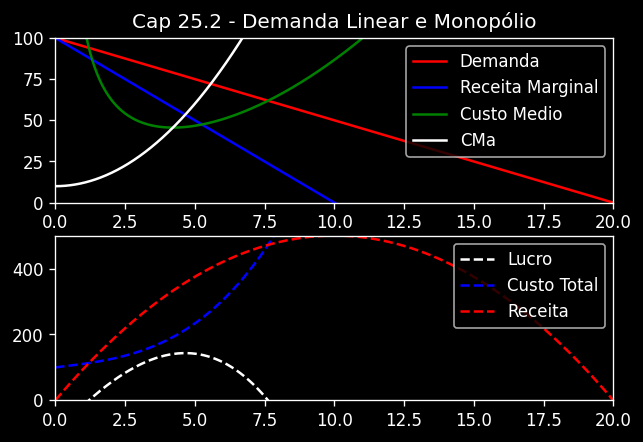
\includegraphics[scale=0.7]{cap25_2-demanda_linear_e_monopolio.png}
	\end{center}
	
\end{frame}

\begin{frame}
	\frametitle{Curva de Demanda Linear e Monopólio}

	Conseguimos ver que a curva de lucro tem um ponto de máximo exatamente onde a curva da receita marginal encontra o custo marginal. Qualquer ponto diferente desse levaria a um nível de lucro menor.
	\\~\\
	Além disso, também é relevante o fato da curva de custo médio estar abaixo da curva de demanda. Se o ponto de produção cuja receita marginal é igual ao custo marginal tiver um custo médio superior a demanda, a empresa receberá menos do que os custo de produção.
\end{frame}

%%%%%%%%%%%%%%%%%%%%%%%%%%%%%%%%%%%%%%%%%%%

\begin{frame}
	\frametitle{Estabelecimento de Preços com Markup}
	
	Agora que tornamos a receita marginal endógena, podemos ver as condições de maximização do lucro quando a firma tem poder de definir o preço ou a quantidade do mercado (mas não os dois ao mesmo tempo).
	\\~\\
	Podemos compreender essa última equação como uma política de preço do monopolista. Para isso, só precisamos isolar o termo $p(y)$ via rearranjo da última equação, o que após feito nos dá a seguinte relação

	$$ p(y) = \frac{CMa(y)}{1 - 1/|\epsilon(y)|} $$

	Essa equação nos diz que o preço praticado no mercado cujo monopolista atua sempre se comportará como uma função de \textit{markup} do seu custo marginal.
\end{frame}

\begin{frame}
	\frametitle{Estabelecimento de Preços com Markup}

	Podemos simplificar a visualização disso do seguinte modo
	
	$$ p(y) = \phi \times CMa(y) $$
	
	onde $\phi = \frac{1}{1 - 1/|\epsilon(y)|}$.
	\\~\\
	Como sabemos, o monopolista sempre operará nos pontos cuja demanda é elástica, isso nos dará um $\epsilon(y) > 1$. Isso nos diz que o divisor $(1 - 1/|\epsilon|) <  1$, o que por sua vez, nos diz que $\phi > 1$.

	\begin{block}{Para dicussão em aula - Varian pg 634}
		Vamos analisar o caso da modelagem para um mercado com demanda de elasticidade constante.
	\end{block}
\end{frame}

%%%%%%%%%%%%%%%%%%%%%%%%%%%%%%%%%%%%%%%%%%%

\begin{frame}
	\frametitle{A Ineficiência do Monopólio}
	
	Já conseguimos ver que, quando uma empresa opera como um monopólio, o preço de mercado será definido sempre acima do seu custo marginal.
	\\~\\
	No mercado de competição perfeita, esse preço seria exatamente igual ao custo marginal. 
	\\~\\
	Isso implica na redução de algum excedente dos consumidores, mas em um incremento no excedente do produtor.
	\\~\\
	Como já sabemos, um arranjo é eficiente no sentido de Pareto se, e somente se, é possível realizar alguma troca de modo a se ter um aumento no excedente de uma das partes sem a redução do excedente de outra parte.
\end{frame}

\begin{frame}
	\frametitle{A Ineficiência do Monopólio}
	
	Agora vamos investigar se o equilíbrio no mercado monopolista é eficiente. Considere a imagem abaixo.
	\begin{center}
		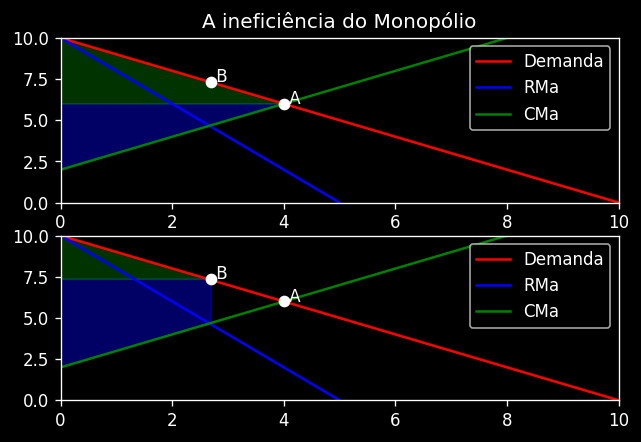
\includegraphics[scale=0.6]{cap25_4-inef_monopolio.png}
	\end{center}
\end{frame}

\begin{frame}
	\frametitle{A Ineficiência do Monopólio}
	
	O gráfico da parte de cima é o equilíbrio no mercado de competição e o de baixo é o nosso equilíbrio com monopólio.
	\\~\\
	Perceba como há um incremento no excedente do produtor (medido pela área azul) e uma redução do excedente do consumidor (área verde).
	\\~\\
	Para investigarmos se há uma ineficiência no sentido de Pareto no ponto $B$, façamos a seguinte pergunta: 
	\begin{block}{Para discussão em aula}
		É possível adicionar uma unidade de produto no mercado de modo que o custo marginal pela produção desse bem seja inferior ao preço do mesmo?
	\end{block}	
\end{frame}

\begin{frame}
	\frametitle{A Ineficiência do Monopólio}
	
	No nível $B$, a curva de preço (medida pela demanda inversa) ainda é superior à curva de custo marginal (aquela reta verde).
	\\~\\
	Desse modo, se o monopolista produzisse mais uma unidade, ele receberia mais do que o custo marginal dessa unidade e os consumidores cujo preço de reserva é igual ao novo nível de preço passariam a consumir o produto.
	\\~\\
	Como o produtor teria um lucro positivo (pois o custo marginal é inferior ao preço) e os consumidores teriam um aumento de excedente, achamos uma melhoria de Pareto.
	\\~\\
	Com isso, podemos ver que o equilíbrio com monopólio é ineficiente no sentido de Pareto.
\end{frame}

%%%%%%%%%%%%%%%%%%%%%%%%%%%%%%%%%%%%%%%%%%%

\begin{frame}
	\frametitle{O Ônus do Monopólio}
	
	Agora que já vimos que o monopólio é ineficiente, podemos querer mensurar o tamanho dessa ineficiência.
	\\~\\
	Uma maneira possível de medir essa ineficiência é observando os excedentes nos cenários competitivo e de monopólio. Observe a figura abaixo:
	
	\begin{center}
		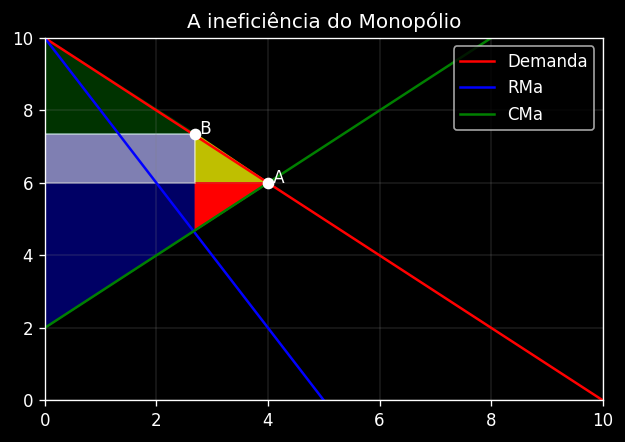
\includegraphics[scale=0.5]{cap25_5-onus_monopolio.png}
		\end{center}
\end{frame}

\begin{frame}
	\frametitle{O Ônus do Monopólio}
	
	A área amarela é a medida da redução do excedente do consumidor.
	\\~\\
	Em vermelho temos a redução do excedente do produtor.
	\\~\\
	Em branco temos o quanto o monopolista consegue "capturar"\ do excedente dos consumidores ao adotar o nível de produção que maximiza o seu lucro.
	\\~\\
	O \textbf{ônus resultante do monopólio} é precisamente a soma das áreas amarela e vermelha.
\end{frame}

%%%%%%%%%%%%%%%%%%%%%%%%%%%%%%%%%%%%%%%%%%%

\begin{frame}
	\frametitle{O Monopólio Natural}

	Já aprendemos o modelo de decisão do monopolista e também já vimos a ineficiência que esse modelo acarreta para os mercados.
	\\~\\
	Ao percebemos que o monopólio produz aquém da quantidade ótima, poderíamos nos sentir tentados a propor regulações que obrigassem o monopolista a aumentar o seu nível de produção até o nível da competição perfeita.
	\\~\\
	Contudo, esse problema é mais complexo do que parece, porque essa proposta de solução não leva em consideração a estrutura de custos.
	\\~\\
	A próxima imagem é um exemplo do que acontece quando alteramos apenas o custo fixo em 3 diferentes cenários.
\end{frame}

\begin{frame}
	\frametitle{O Monopólio Natural}
	\begin{center}
		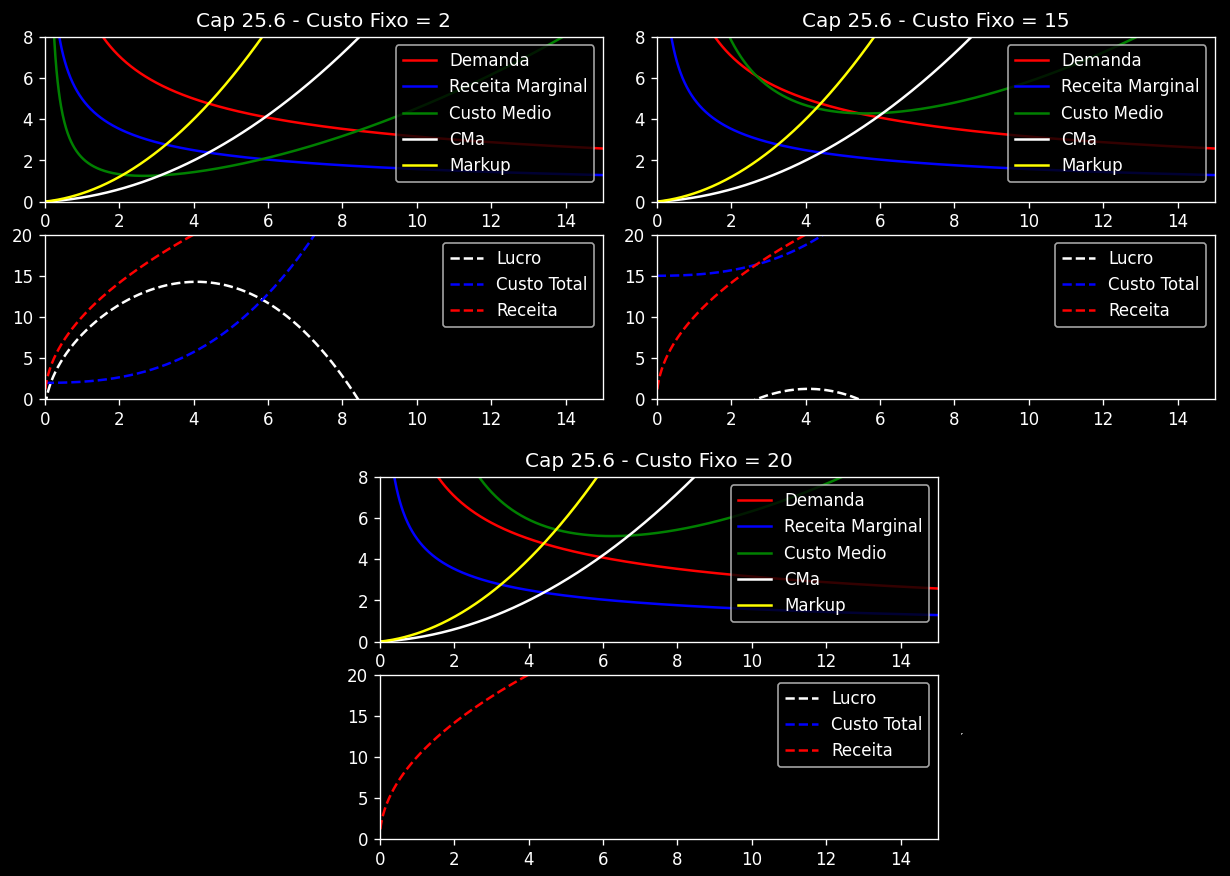
\includegraphics[scale=0.3]{cap25_6-monopolio_natural.png}
		\end{center}
\end{frame}

\begin{frame}
	\frametitle{O Monopólio Natural}

	Chamamos de \textbf{monopólio natural} a situação onde temos uma estrutura de custo fixos muito alta e custos marginais baixos.
	\\~\\
	Agora podemos ver que se obrigarmos o monopolista a produzir o nível da competição perfeita, pode acontecer do projeto não ser sustentável, pois a curva de custo médio está acima da curva de demanda.
	\\~\\
	Não existe solução simples para essa questão. Na maioria das situações os monopólios naturais são regulamentados ou operados diretamente pelos governos.
	\\~\\
	Cada opção de solução acaba acarretando benefícios e malefícios consigo. Em ambos os casos, os problemas são geralmente oriundos devido a informação assimétrica entre a empresa e os seus controladores.
\end{frame}

%%%%%%%%%%%%%%%%%%%%%%%%%%%%%%%%%%%%%%%%%%%

\begin{frame}
	\frametitle{O que Causa os Monopólios?}

	Agora nos resta uma última investigação: Qual a causa dos monopólios?
	\\~\\
	Uma variável que podemos creditar como importante é a \textbf{escala mínima de eficiêntia (EME)}. Ela nada mais é do que o ponto de mínimo da nossa curva de custo médio.
	\\~\\
	O formato da curva de custo médio (e consequentemente a EME) é definido exclusivamente pela tecnologia.
	\\~\\
	Quando temos uma escala mínima de eficiência muito elevada, uma empresa precisa produzir uma quantidade muito grande dos bens vendidos no mercado para se manter.
\end{frame}

\begin{frame}
	\frametitle{O que Causa os Monopólios?}
	Quando temos uma EME pequena, qualquer empresa pequena pode começar a operar no mercado. Isso aumenta o número de competidores.
	\\~\\
	O que acaba por reduzir o peso de cada empresa individualmente. O que acaba por gerar um ambiente de competição.
	\\~\\
	Observe que o fator importante é a relação entre a EME e o tamanho do mercado. Se a EME é de 10.000 unidades, mas o mercado é o país todo, essa é uma EME relativamente baixa. Se o tamanho do mercado fosse um único shopping center, aí seria considerar consideravelmente alta.
\end{frame}

\begin{frame}
	\frametitle{O que Causa os Monopólios?}
	Além da EME, outra maneira de se criar um monopólio é por meio da coordenação dos agentes ofertantes em uma \textbf{colusão}.
	\\~\\
	Quando um conjunto de empresa se une para definir em conjunto a produção, elas agem como um \textbf{cartel}.
	\\~\\
	Esse cartel acaba atuando como se fosse um ofertante só (e consequentemente, age com o poder de mercado advindo dessa coordenação).
\end{frame}

\begin{frame}
	\frametitle{O que Causa os Monopólios?}
	Um terceiro e último motivo para o nascimento de um monopólio é o bom e velho "cheguei primeiro".
	\\~\\
	Se uma empresa, por algum acidente histórico, é a primeira a se estabelecer no mercado. É natural que ela se valha da falta de competidores e consiga um crescimento em escala.
	\\~\\
	Quando novos ofertantes entram no mercado, o monopolista consegue usar seu arsenal de escala e reduzir artificialmente o preço até o ponto onde ninguém além dele pode se manter.
\end{frame}

%%%%%%%%%%%%%%%%%%%%%%%%%%%%%%%%%%%%%%%%%%%
\section[C.Monopólio]{Comportamento do Monopólio}
%%%%%%%%%%%%%%%%%%%%%%%%%%%%%%%%%%%%%%%%%%%

\begin{frame}
	\huge O comportamento do Monopolista \normalsize
	\\~\\
	\begin{itemize}
		\item Tipos de discriminação de preços
		\item Discriminação de 1º ordem
		\item Discriminação de 2º ordem
		\item Discriminação de 3º ordem
		\item Vinculação de produtos
		\item Tarifas bipartidas
		\item Competição monopolística
		\item Estabilidade na Competição
		\item Diferenciação de Produtos
		\item Mais sorveteiros
	\end{itemize}
\end{frame}

%%%%%%%%%%%%%%%%%%%%%%%%%%%%%%%%%%%%%%%%%%%

\begin{frame}
	\frametitle{Tipos de Discriminação de Preços}

	Nós vimos que o monopolista acaba produzindo em um ponto onde a demanda ainda está disposta a pagar por mais do que o custo marginal.
	\\~\\
	Porque o monopolista não abaixa o preço para vender mais unidades?
	\\~\\
	Ele teria de baixar o preço de todos os produtos e não apenas os adicionais!
	\\~\\
	Existem alguns monopolistas que detém o poder de \textbf{discriminação de preços}.

\end{frame}

\begin{frame}
	\frametitle{Tipos de Discriminação de Preços}

	\begin{itemize}
		\item Discriminação de Preços de 1º Grau:
			\begin{itemize}
			\item[] Nesse caso ele tem poder de cobrar um preço diferente para cada consumidor e para cada quantidade.
			\end{itemize}
		\item Discriminação de Preços de 2º Grau
			\begin{itemize}
			\item[] Nesse caso ele tem poder de discriminar o preço apenas para as quantidades compradas. Mas todos os consumidores que levarem a mesma quantidade, pagarão o mesmo preço no total.
			\end{itemize}
		\item Discriminação de Preços de 3º Grau
			\begin{itemize}
			\item[] Esse é o caso mais comum. É quando o monopolista tem o poder de escolher qual preço cada pessoa vai pagar por todas as unidades que levar. Ou seja, ele pode controlar qual o valor de todas as unidades da cesta, contudo, não pode diferenciar o valor entre essas unidades.
			\end{itemize}
		\end{itemize}

\end{frame}

%%%%%%%%%%%%%%%%%%%%%%%%%%%%%%%%%%%%%%%%%%%

\begin{frame}
	\frametitle{Discriminação de Preços de 1º Grau}

	O monopolista está em plenos poderes. Ele possui conhecimento do preço de reserva de cada consumidor e, com esse conhecimento, cobra exatamente o valor máximo para cada quantidade. Também chamamos esse tipo de \textbf{discriminação perfeita}.
	\\~\\
	Um fato curioso desse arranjo é que, por incrível que pareça, ele é eficiente no sentido de Pareto.
	
	\begin{block}{Para discussão em aula}
		Quem pode explicar como esse arranjo pode ser ótimo de Pareto?
	\end{block}

	Em termos de excedente, o que acontece é que o monopolista captura todo o excedente do mercado. Os consumidores, por sua vez, não possuem nenhum excedente.
\end{frame}

\begin{frame}
	\frametitle{Discriminação de Preços de 1º Grau}

	\begin{figure}[H]
		\centering
		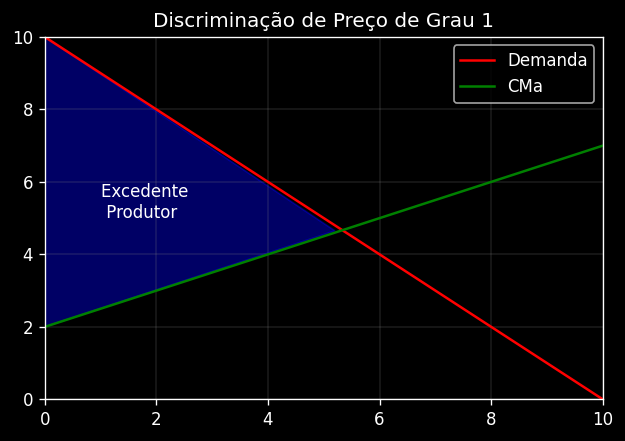
\includegraphics[scale=0.75]{cap26_2-discriminacao_grau1.png}
	\end{figure}

\end{frame}

\begin{frame}
	\frametitle{Discriminação de Preços de 1º Grau}

	Um exemplo é o mafioso Don Vito Corleone da clássica trilogia de filmes The Godfather. O "modelo de negócio"\ do protagonista é fazer alguns favores em troca de outros favores. No caso do personagem mafioso, ele abusava do poder de mercado que detinha para cobrar o máximo possível (em bens ou serviços) de quem estava em dívida com ele.

	\begin{figure}[H]
		\centering
		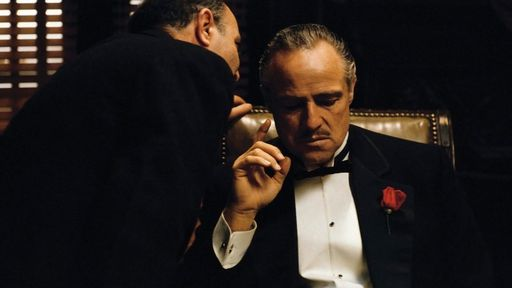
\includegraphics[scale=0.3]{cap26_2-don_corleone.jpeg}
	\end{figure}

\end{frame}

\begin{frame}
	\frametitle{Discriminação de Preços de 2º Grau}

	Nesse modelo, também chamado de \textbf{fixação de preços não linear}, o produtor já não pode cobrar, por uma mesma quantidade, um valor diferente entre consumidores diferentes.
	\\~\\
	Isso força o monopolista a desenvolver uma estratégia de precificação que tente tirar o maior proveito possível das diferentes curvas de demanda.
	\\~\\
	Imagine que temos apenas 2 grupos de consumidores no mercado. Como nosso modelo prevê, o monopolista tem acesso as curvas de demanda de cada consumidor, mas como limitação, ele só pode escolher quais cestas ofertar por qual preço, e deixar que os consumidores escolham qual é a melhor para eles.

\end{frame}

\begin{frame}
	\frametitle{Discriminação de Preços de 2º Grau}

	O objetivo do monopolista é captar todo o excedente do mercado. Mas ele enfrenta uma limitação nessa modalidade de discriminação de preços.
	\\~\\
	Como ele não pode vender a mesma quantidade a preços diferentes para os grupos de consumidores, ele tem de escolher se vai vender a preço de reserva da curva de demanda 1 ou 2.
	\\~\\
	Se ele optar por vender na fronteira da curva de demanda 1, ele vai abrir mão de todo o excedente advindo dos consumidores do tipo 2!

\end{frame}

\begin{frame}
	\frametitle{Discriminação de Preços de 2º Grau}

	\begin{figure}[H]
		\centering
		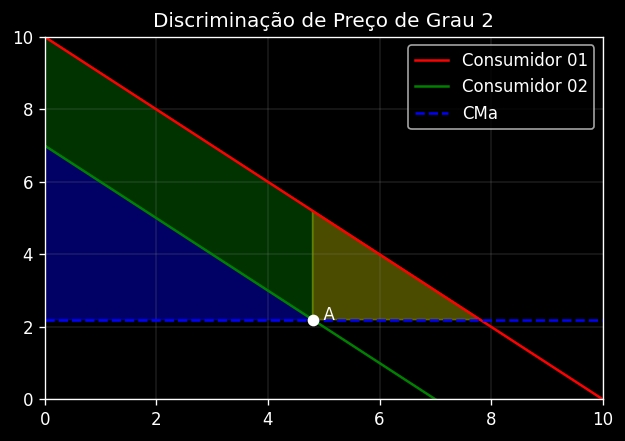
\includegraphics[scale=0.7]{cap26_3-discriminacao_grau2_1.png}
	\end{figure}
	
\end{frame}

\begin{frame}
	\frametitle{Discriminação de Preços de 2º Grau}

	\begin{figure}[H]
		\centering
		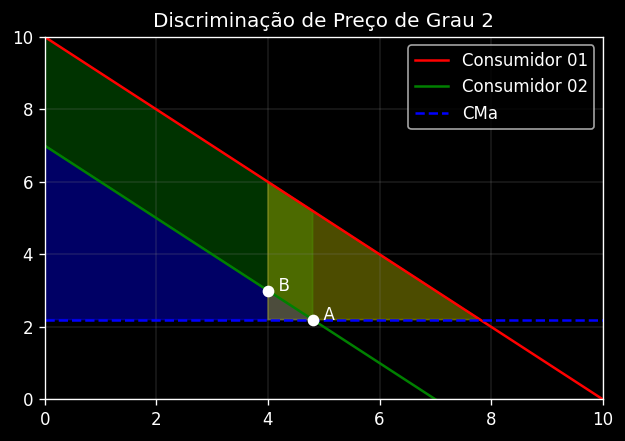
\includegraphics[scale=0.7]{cap26_3-discriminacao_grau2_2.png}
	\end{figure}
	
\end{frame}

\begin{frame}
	\frametitle{Discriminação de Preços de 2º Grau}

	\begin{figure}[H]
		\centering
		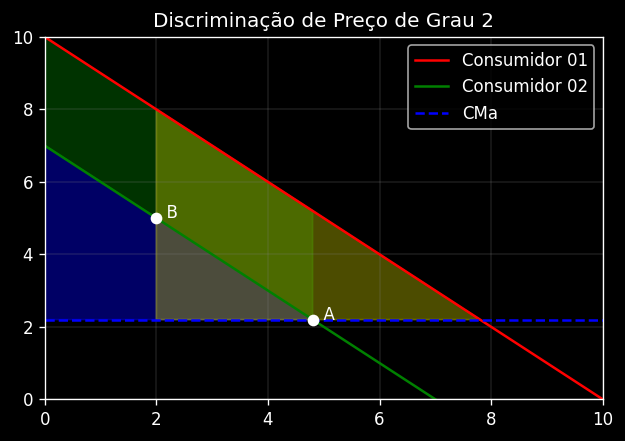
\includegraphics[scale=0.7]{cap26_3-discriminacao_grau2_3.png}
	\end{figure}
	
\end{frame}

\begin{frame}
	\frametitle{Discriminação de Preços de 2º Grau}

	Na realidade, o principal método de incentivo a autosseleção é a alteração da qualidade do bem. Normalmente, o monopolista reduz a qualidade dos produtos direcionados aos consumidores com preços de reserva menores, afim de evitar que seus consumidores dispostos a pagar mais, prefiram comprar esses produtos ao invés de produtos de "primeira linha".
	\\~\\
	Essa estratégia maximiza o lucro do monopolista e ainda garante algum excedente para os consumidores das demandas mais altas.

	\begin{figure}[H]
		\centering
		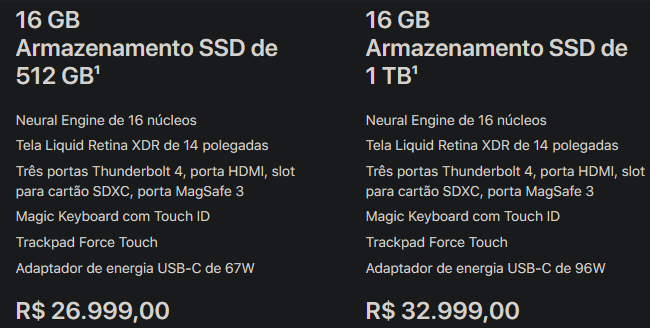
\includegraphics[scale=0.3]{cap26_3-discriminacao_grau2_4.png}
	\end{figure}

\end{frame}

%%%%%%%%%%%%%%%%%%%%%%%%%%%%%%%%%%%%%%%%%%%

\begin{frame}
	\frametitle{Discriminação de Preços de 3º Grau}

	Nesse caso, o monopolista consegue discernir claramente qual consumidor pertence a qual grupo e, consequentemente, consegue cobrar um preço diferente. Atente para o fato que o monopolista só pode adota um único preço para cada grupo de consumidores.
	\\~\\
	Na prática, a modelagem desse problema é muito parecida com o que vimos no capítulo passado, já que, ele só pode escolher um único preço para cada tipo de consumidor.
	\\~\\
	A única diferença do modelo do capítulo passado é que ele vai se deparar com mais de uma curva de demanda.

\end{frame}

\begin{frame}
	\frametitle{Discriminação de Preços de 3º Grau}

	\begin{center}
		\LARGE $\stackrel{max}{\text{\small $y_1,y_2$}} \ \  \stackrel{p_1(y_1)y_1 + p_2(y_2)y_2 - c(y_1 + y_2)}{\ }$ \\
	\end{center}

	$$ RM_1(y_1) = CMa(y_1+y_2) $$
	$$ RM_2(y_2) = CMa(y_1+y_2) $$

	\begin{center}
		Isso claramente implica em
	\end{center}

	$$ RM_1(y_1) = RM_2(y_2) = CMa(y_1+y_2) $$

\end{frame}

\begin{frame}
	\frametitle{Discriminação de Preços de 3º Grau}

	Podemos usar a nossa fórmula da elasticidade para elaborar um pouco mais esse problema:

	$$ p_1(y_1) \left[1 - \frac{1}{|\epsilon_1(y_1)|} \right] = CMa(y_1 + y_2) $$
	$$ p_2(y_2) \left[1 - \frac{1}{|\epsilon_2(y_2)|} \right] = CMa(y_1 + y_2) $$

	Suponha que $y_1 = y_2$. Se $p_1 > p_2$, então:

	$$ 1 - \frac{1}{|\epsilon_1(y_1)|} < 1 - \frac{1}{|\epsilon_2(y_2)|} $$

\end{frame}

\begin{frame}
	\frametitle{Discriminação de Preços de 3º Grau}

	O que implica em

	$$ \frac{1}{|\epsilon_1(y_1)|} > \frac{1}{|\epsilon_2(y_2)|} $$

	Que, por fim, nos diz que

	$$ |\epsilon_1(y_1)| < |\epsilon_2(y_2)| $$

\end{frame}

\begin{frame}
	\frametitle{Discriminação de Preços de 3º Grau}

	Vocês agora entendem o motivo de existir meia entrada.
	\\~\\
	Eu sei, eu sei, isso é muito top.
	\\~\\
	O monopolista vai cobrar mais caro de quem tiver a demanda menos elástica.

\end{frame}

\begin{frame}
	\frametitle{Discriminação de Preços de 3º Grau}

	\begin{figure}[H]
		\centering
		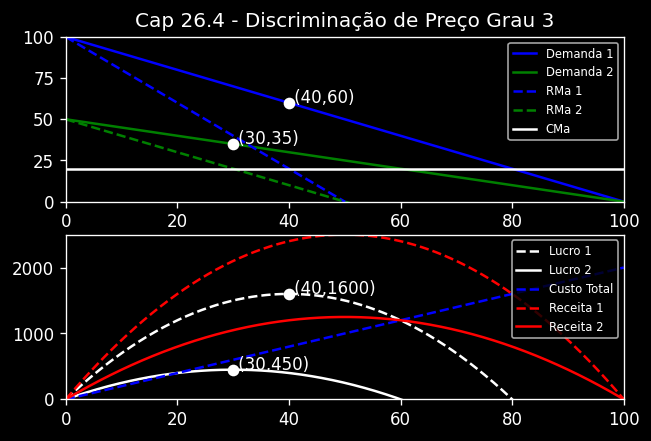
\includegraphics[scale=0.7]{cap26_4-discriminacao_grau3.png}
	\end{figure}

\end{frame}

\begin{frame}
	\frametitle{Discriminação de Preços de 3º Grau}

	\begin{figure}[H]
		\centering
		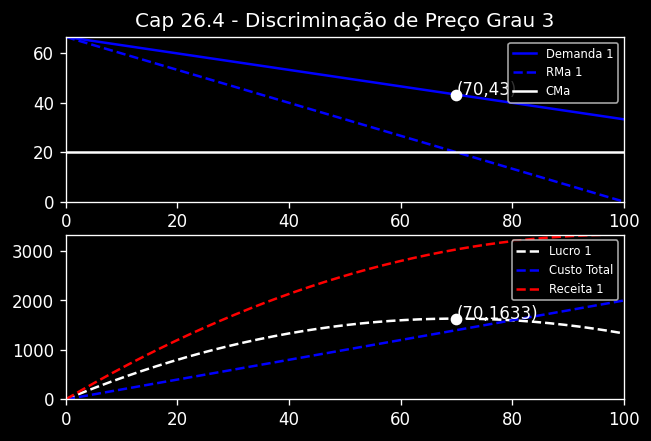
\includegraphics[scale=0.7]{cap26_4-discriminacao_grau3_2.png}
	\end{figure}

\end{frame}

%%%%%%%%%%%%%%%%%%%%%%%%%%%%%%%%%%%%%%%%%%%

\begin{frame}
	\frametitle{Vinculação de Produtos}

	Já vimos que a vontade do monopolista é cobrar o máximo possível para cada cliente em cada quantidade. Isso faria com que ele capturasse todo o excedente do mercado. 
	\\~\\
	Como na prática isso implicaria em conhecimento perfeito de todos os consumidores e existe uma legislação que limita a capacidade de impor muito do poder de mercado, as empresas se valem de estratégias para maximizar esse excedente.
	\\~\\
	Uma dessas estratégias é exatamente a venda casada. A ideia é a seguinte: como o vendedor não pode cobrar um preço para cada consumidor, ele precisa ter uma ideia dos preços de reserva dos mesmos para que possa cobrar exatamente o valor do preço de reserva mais baixo que o custo marginal permita.

\end{frame}

\begin{frame}
	\frametitle{Vinculação de Produtos}

	\begin{center}
		\begin{tabular}{ |c|c|c| } 
		 \hline
		 Consumidor & Processador Texto & Planilha Eletrônica \\ 
		 \hline
		 A & 120 & 100 \\ 
		 B & 100 & 120 \\ 
		 \hline
		\end{tabular}
	\end{center}

	\begin{block}{Para discussão em aula}
		Vale mais a pena o monopolista cobrar separadamente ou pela cesta dos dois bens?
	\end{block}

\end{frame}

%%%%%%%%%%%%%%%%%%%%%%%%%%%%%%%%%%%%%%%%%%%

\begin{frame}
	\frametitle{Tarifas Bipartidas}

	Baseado no paper de Walter Oi, "A Disneyland Dilemma: Two-Part Tariffs for a Mickey Mouse Monopoly".
	\\~\\
	Como o monopolista se comportará no caso da venda de dois produtos que possuem demandas interrelacionadas?
	\\~\\
	No tópico anterior, supomos que as demandas eram independentes. Agora temos um caso onde, ao aumentar a oferta do bem 1, os consumidores estarão menos propensos a consumir o bem 2. Chamamos esse arranjo de \textbf{tarifa bipartida}.

\end{frame}

\begin{frame}
	\frametitle{Tarifas Bipartidas}

	Como já trabalhamos antes, sabemos que a maximização do lucro é obtida no ponto onde o custo marginal é igual à receita marginal. 
	\\~\\
	Fazendo isso para a oferta do bem 1 e como ele não pode discriminar perfeitamente os preços, haverá um excedente do consumidor. Esse excedente é exatamente o valor máximo que ele pode cobrar pelo bem 2. 
	\\~\\
	Nesse caso, pode ser que a quantidade cobrada pelo bem 2 seja inferior ao montante que iguale o custo marginal à receita marginal.
\end{frame}

\begin{frame}
	\frametitle{Tarifas Bipartidas}

	\begin{figure}[H]
		\centering
		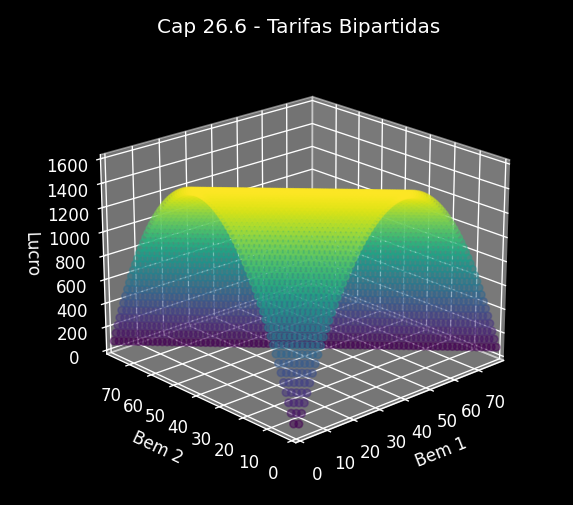
\includegraphics[scale=0.7]{cap26_6-tarifas_bipartidas3.png}
	\end{figure}

\end{frame}

%%%%%%%%%%%%%%%%%%%%%%%%%%%%%%%%%%%%%%%%%%%

\begin{frame}
	\frametitle{Competição Monopolística}

	Nós começamos essa seção do livro partindo da posição oposta aos modelos que vimos ao longo da primeira metade do curso.
	\\~\\
	Adaptamos o modelo da escolha maximizadora do lucro para a existência do poder de mercado e avançamos como o monopolista pode usar esse poder mesmo em arranjos menos favoráveis à capacidade de discriminação de preços.
	\\~\\
	Nessas últimas duas seções expandimos nosso modelo para mais de um produto e como eles podem interagir entre si para a maximização do lucro.

\end{frame}

\begin{frame}
	\frametitle{Competição Monopolística}

	Até agora, tratamos uma \textbf{indústria} como um conjunto de produtores cujo resultado do esforço produtivo era \textit{exatamente} a mesma mercadoria. Isso quer dizer que, sendo 1 (que é o caso do monopólio) ou 1.000 produtores, todas as mercadorias que saem das fábricas e são comercializadas seriam exatamente as mesmas. 
	\\~\\
	Essa hipótese simplificadora vai dar lugar a uma nova que, na minha opinião, é bem mais aplicável a nossa realidade fática.
	\\~\\
	Os produtos agora possuem certas propriedades exclusivas (sendo a marca a principal) e seus competidores também serão diferenciáveis entre si. Todos competindo por um mercado de bens relativamente parecidos aos consumidores.

\end{frame}

\begin{frame}
	\frametitle{Competição Monopolística}

	Nesse novo arranjo, os produtores possuem características de ambos os modelos vistos. 
	\\~\\
	Eles não podem alterar seus preços completamente como um monopólio, porque os consumidores olhariam para os seus concorrentes e comprariam algum produto semelhante ao seu, só que mais barato. 
	\\~\\
	Por outro lado, eles não estão fadados estritamente ao preço de mercado, uma vez que nesse arranjo a demanda não será infinitamente elástica. 
	\\~\\
	O nome dessa estrutura setorial é \textbf{concorrência monopolística}.

\end{frame}

\begin{frame}
	\frametitle{Competição Monopolística}

	É razoável supor que se o número de concorrentes aumentar (algo que está muito relacionado às barreiras de entrada) haverá impactos na curva de demanda que a empresa está imposta.
	\\~\\
	O primeiro impacto que podemos supor é que essa curva irá se aproximar mais da origem do plano cartesiano. Ou seja, ele vai acabar tendo que baixar mais o seu preço se quiser continuar vendendo a mesma quantidade.
	\\~\\
	O segundo impacto previsto é que a elasticidade de demanda aumentará porque agora os consumidores podem escolher mais opções em relação a antes.

\end{frame}

\begin{frame}
	\frametitle{Competição Monopolística}

	Se todas as empresas do mercado tiverem como objetivo o lucro. Qualquer equilíbrio alcançado terá que obedecer algumas restrições:

	\begin{itemize}
		\item Cada empresa venderá o máximo possível. Ou seja, elas sempre optam por ofertar cestas que estejam na curva de demanda e não abaixo dela.
		\item Cada empresa precisará maximizar seu lucro levando em consideração as imposições oriundas à sua curva de demanda da empresa.
		\item Quanto mais competidores o mercado tiver, mais próximo de zero será o lucro das empresas contidas no mercado.
	\end{itemize}

\end{frame}

\begin{frame}
	\frametitle{Competição Monopolística}

	Do fato 1, podemos derivar o fato que quaisquer opções de maximização estão na própria curva de demanda.
	\\~\\
	Do fato 3, podemos ver que a medida que o número de competidores tende ao infinito, a cesta escolhida deve ser num ponto onde a curva de custo médio tangencia a curva de demanda.
	\\~\\
	Por fim, o nosso postulado 2 afirma que a maximização ocorrerá na curva de demanda, isso implica no fato que a curva de custo médio não cruzará a curva de demanda, porque se isso acontecer, as empresas terão lucro positivos.
\end{frame}

%%%%%%%%%%%%%%%%%%%%%%%%%%%%%%%%%%%%%%%%%%%

\begin{frame}
	\frametitle{Estabilidade na Competição}

	Esse seção é inspirada no clássico artigo de 1929 "Stability in Competition"\ de Harold Hotelling. Isso mesmo, 1929.
	\\~\\
	Imagine que a orla da Ponta Negra seja retilínea e que só seja permitida a venda de sorvetes mediante autorização da Prefeitura. Adicionaremos a restrição que a probabilidade de você encontrar um transeunte com calor é uniforme em toda a extensão da orla. Suporemos também que os preços dos sorvetes sempre serão iguais, que não há diferença de qualidade e que por motivos climáticos só exista um único sabor disponível.
	\\~\\
	Diante das características do mercado acima, onde o primeiro sorveteiro com licença da prefeitura deve instalar sua barraquinha?. Não é difícil chegar na conclusão que ele deve se instalar exatamente no meio da orla.

\end{frame}

\begin{frame}
	\frametitle{Estabilidade na Competição}

	Supondo que outro sorveteiro consiga sua licença para vender na orla. Qual será o melhor arranjo? Se usarmos o mesmo pensamento de antes, podemos supor que cada vendedor fique no ponto que corresponda a 1/4 e 3/4 do tamanho da orla.
	\\~\\
	No final teremos uma distância máxima de 1/4 da orla para cada consumidor e 1/2 da receita total para cada sorveteiro.
	\\~\\
	Como eles querem maximizar sua receita, cada vendedor terá o incentivo à se mover um pouco para o centro, porque desse modo ele manterá a sua demanda cativa e ainda "roubará"\ parte da demanda do seu colega de ofício.

\end{frame}

\begin{frame}
	\frametitle{Estabilidade na Competição}

	No final, ambos se encontrarão no centro da orla. Esse novo arranjo aumenta a distância máxima dos consumidores para 1/2 e mantém a receita dos sorveteiros em 1/2.
	\\~\\
	Esse é um exemplo de como a competição pelos clientes gerou um padrão menos eficiente na localização dos sorveteiros. Quanto menos agentes temos nos mercado, mais precisaremos nos preocupar com as estratégias que cada um deles adotará.
	\\~\\
	Se você começou a pensar em teoria do jogos, é isso mesmo!
\end{frame}

%%%%%%%%%%%%%%%%%%%%%%%%%%%%%%%%%%%%%%%%%%%

\begin{frame}
	\frametitle{Diferenciação de Produtos}

	Existem situações onde os produtores optam por buscar o oposto do modelo de convergência, eles investem na diferenciação dos seus produtos. Qual o sentido disso? nós já vimos que, quanto maior é o grau de diferenciação do produto, mais característica de monopólio o competidor terá.
	\\~\\
	Infelizmente, o livro não adentra muito além da demonstração que existe essa vertente de possibilidade dos mercados.
	\\~\\
	O importante aqui é saber que a competição monopolística pode gerar tanto uma padronização dos produtos quanto uma excessiva diferenciação deles.

\end{frame}

%%%%%%%%%%%%%%%%%%%%%%%%%%%%%%%%%%%%%%%%%%%
\section[M.Fatores]{Mercado de Fatores}
%%%%%%%%%%%%%%%%%%%%%%%%%%%%%%%%%%%%%%%%%%%

\begin{frame}
	\huge O Mercado de Fatores \normalsize
	\\~\\
	\begin{itemize}
		\item O Monopólio no Mercado do Produto
		\item O Monopsônio
		\item Monopólios Upstream e Downstream na Cadeia de Produção
	\end{itemize}
\end{frame}

\begin{frame}
	\frametitle{O Monopólio no Mercado do Produto}

	Agora que temos um \textit{framework} mais interessante como o comportamento do monopolista. Podemos pensar nas implicações para o mercado de fatores. Veremos algumas situações:
	\\~\\
	\begin{enumerate}
		\item Qual a diferença entre a demanda por fatores de um monopólio e de uma empresa competitiva.
	
		\item O que acontece quando temos um mercado de fatores competitivo mas apenas um comprador\footnote{O nome desse arranjo é \textbf{monopsônio}.}.
	
		\item Como será o arranjo onde há um monopolista no mercado de fatores e um monopolista no mercado de produto.
	\end{enumerate}
\end{frame}

\begin{frame}
	\frametitle{O Monopólio no Mercado do Produto}

	Pensemos novamente na empresa que demanda fatores de produção. 
	\\~\\
	Sua demanda maximizadora será dada pelo ponto onde o custo marginal pela compra do fator é igual à receita marginal advinda do emprego desse fator.
	\\~\\
	Sua função de produção será dada por $y = f(x)$. 
	\\~\\
	A receita será dada pelo volume de produção e da demanda inversa do mercado, algo como, $R(y) = p(y)y$. 

\end{frame}

\begin{frame}
	\frametitle{O Monopólio no Mercado do Produto}
	
	O \textbf{Produto Marginal} de um fator de produção é obtido pela variação da função produção em relação à variação do fator observado. No nosso exemplo, só temos um único fator, então:

	$$ PM_x = \frac{\delta y}{\delta x} = f'(x) $$

	Como não é novidade, esse incremento marginal na produção será vendido e produzirá uma \textbf{Receita Marginal}. 
	\\~\\
	Podemos expor esse efeito pela expressão da  variação infinitesimal da receita dividida pela variação infinitesimal do produto.

	$$ RM_y = \frac{\delta R}{\delta y} = p(y) + p'(y)y $$

\end{frame}

\begin{frame}
	\frametitle{O Monopólio no Mercado do Produto}
	
	Até agora já vimos o impacto que um fator causa no produto e, do outro lado, o impacto que um produto causa na receita. Agora nos resta fazer a relação direta entre essas duas lógicas.
	\\~\\
	Uma vez que $y = f(x)$, então, $p(y) = p(f(x))$. Podemos reescrever nossa equação da receita como:

	$$ R(x) = p(f(x))f(x) $$

	Agora que temos nossa função de receita explicitamente relacionada ao nosso fator de produção, podemos obter a relação chamada de \textbf{Produto da Receita Marginal} que mede o impacto na receita dada uma variação no fator de produção.

\end{frame}

\begin{frame}
	\frametitle{O Monopólio no Mercado do Produto}

	Para obter-la usamos a derivada de $R(x)$ em relação à $x$.
	\\~\\
	A regra da cadeia para $p(y) = p(f(x))$ nos diz que $\frac{d p(y) }{d x} = \frac{d p(y)}{d y} \frac{d y}{d x} $.
	\\~\\
	Temos que aplicar, ao mesmo tempo, a regra da multiplicação junto à regra da cadeia.
	\\~\\
	$$ PRM_x = \frac{d R(x)}{d x} = p(y)f'(x) + f(x)p'(y)f'(x) $$
	$$ = [p(y) + p'(y)y]f'(x) $$
	$$ = RM_y \times PM_x $$

\end{frame}

\begin{frame}
	\frametitle{O Monopólio no Mercado do Produto}

	Ou seja, o impacto na receita de uma variação do fator de produção é igual à receita marginal da produção vezes o produto marginal do fator. O que faz todo sentido.
	\\~\\
	Podemos trazer de volta a nossa expressão da receita marginal desenvolvida na seção de maximização de lucro do capítulo 25. 
	
	$$RM(y) = p(y) \left[ 1 - 1/|\epsilon| \right]$$

	Também acabamos de ver que

	$$PRM_x = RM_y \times PM_x $$

	Juntando as duas equações temos que

	$$ \frac{d R(x)}{d x} = p(y) \left[ 1 - \frac{1}{|\epsilon|} \right] PM_x $$

\end{frame}

\begin{frame}
	\frametitle{O Monopólio no Mercado do Produto}

	Uma vez que, na competição perfeita, a elasticidade é infinita. Isso implica no fato que o produto da receita marginal será dado pelo preço de mercado (que é igual à receita marginal) vezes o produto marginal do fator de produção, ou seja, $p PM_x$. 
	\\~\\
	O professor chamou de \textbf{valor do produto marginal} essa multiplicação entre o preço de mercado e o produto marginal do fator.

	$$ \textrm{Competição Perfeita: } PRM_x = p PM_x $$

	$$ \textrm{Monopólio: } PRM_x = p \left[ 1 - \frac{1}{|\epsilon|} \right] PM_x \leq pPM_x $$

	No caso do monopólio, o produto da receita marginal será, no máximo, igual ao valor do produto marginal.

\end{frame}

\begin{frame}
	\frametitle{O Monopólio no Mercado do Produto}

	O motivo disso é que o monopolista interfere no preço de equilíbrio do mercado ao produzir mais unidades. 
	\\~\\
	Ao chegar no ponto onde a demanda é elástica, o resultado na receita será cada vez menor. 
	\\~\\
	Já no caso da empresa competitiva, não importa quantos produtos ela produza, o preço de mercado sempre será o mesmo.
	\\~\\
	Não é difícil perceber, então, que o monopolista possui menos incentivo à utilizar determinada quantidade de insumo na sua produção.

\end{frame}

\begin{frame}
	\frametitle{O Monopólio no Mercado do Produto}

	Podemos saber \textbf{quanto} será demandado por cada empresa no mercado de fatores de produção? Não é difícil supor que será a quantidade que iguala o produto da receita marginal ao custo marginal desse fator.
	\\~\\
	Se o mercado de fatores é competitivo, uma empresa operando em um mercado igualmente competitivo poderá demandar a quantidade de insumos que desejar ($x_c$) a um preço constante $w$. A quantidade empregada de insumo será:

	$$ \textrm{Competição Perfeita: } PRM_{x_c} = pPM(x_c) = w $$

	Mas no caso do monopolista, ele não demandará a igualdade com o valor do produto marginal.

	$$ \textrm{Monopólio: } PRM(x_m) = w $$
\end{frame}

\begin{frame}
	\frametitle{O Monopólio no Mercado do Produto}

	\begin{figure}[H]
		\centering
		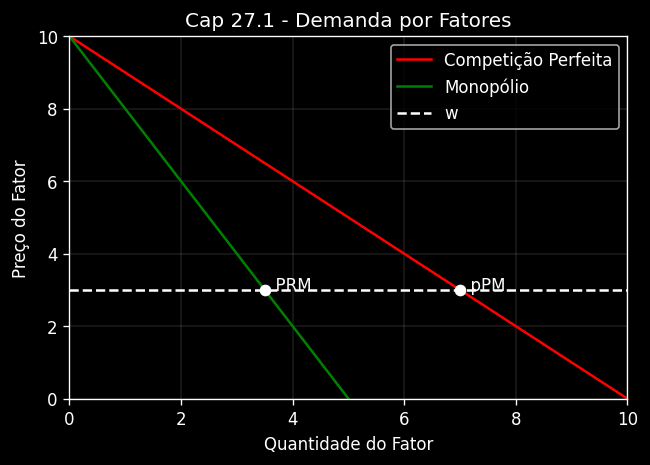
\includegraphics[scale=0.7]{cap27_1-demanda_fatores.png}
	\end{figure}

\end{frame}
%%%%%%%%%%%%%%%%%%%%%%%%%%%%%%%%%%%%%%%%%%%

\begin{frame}
	\frametitle{O Monopsônio}

	Um cenário onde temos um mercado competitivo de fatores, um único comprador de fator e um mercado de produtos competitivo.
	\\~\\
	Para simplificar, vamos supor que a empresa usa apenas um único fator de produção. Sua função de produção será dada por $y = f(x)$.  
	\\~\\
	A análise de comportamento do monopsônio é parecida com a do monopólio, só que ao invés de impactar o mercado pela oferta de bens, o poder de mercado é exercido pela compra. 
	\\~\\
	A quantidade de fator comprado, impactará no preço pago por ele.

\end{frame}

\begin{frame}
	\frametitle{O Monopsônio}

	Para expandir o modelo, vamos criar uma função de oferta inversa $w(x)$ onde o preço pago pelo insumo será determinado pela quantidade demandada pelo nosso único comprador (chamado de \textbf{monopsonista}). É razoável supor que $\frac{d w(x)}{d x} > 0$.
	\\~\\
	Num mercado de fatores competitivo, a curva de oferta de fatores é plana. Ou seja, não importando a quantidade demanda, o custo será sempre o mesmo. 
	\\~\\
	Já no caso de um único comprador, a curva de oferta de fatores será inclinada positivamente.
	\\~\\
	"Uma empresa num mercado de fatores competitivo é uma \textbf{tomadora de preços}. Um monopsionista é um \textbf{fixador de preços}".

\end{frame}

\begin{frame}
	\frametitle{O Monopsônio}

	A maximização de lucro do monoposionista será:

	\begin{center}
	\LARGE $\stackrel{max}{\text{\small $x$}} \ \ 
	\stackrel{pf(x) - w(x)x}{\ }$ \\
	\end{center}

	Ou seja, temos que encontrar a quantidade de insumo - $x$ - que permita maximizar a diferença entre a receita total - $p f(x)$ - e o custo total - $w(x)x$. A condição de primeira ordem desse problema será:

	$$ pf'(x) - [ w(x) + w'(x)x ] = 0 $$
	$$ pf'(x) = w(x) + w'(x)x $$
	$$ \underbrace{pPM_x}_{\textrm{PRM}} = \ \underbrace{w(x) + w'(x)x}_{\textrm{Custo Marginal}} $$

\end{frame}

\begin{frame}
	\frametitle{O Monopsônio}

	Como supomos no início do nosso caso, o mercado do produto é competitivo. Isso quer dizer que a receita marginal será igual a $pPM_x$ (que é a mesma coisa que $pf'(x)$). Mas obter o custo marginal não será tão simples quanto antes.
	\\~\\
	Quando a firma compra uma pequena quantidade ($x$) do fator de produção, ela deve pagar o preço desse fator vezes a quantidade ($wx$). Contudo, nesse caso, o preço será afetado exatamente na quantidade demanda ($w'(x)x$). O valor final pago é a soma dessas duas ações.
	\\~\\
	Podemos desenvolver essa lógica exatamente como desenvolvemos a receita do monopolista na seção 25.1.

\end{frame}

\begin{frame}
	\frametitle{O Monopsônio}

	$$ \Delta c = w \Delta x + x \Delta w $$
	$$ \frac{\Delta c}{\Delta x} = w + x \frac{\Delta w}{\Delta x} $$
	$$ = w \left[ 1 + \frac{x}{w} \frac{\Delta w}{\Delta x} \right] $$
	$$ = w \left[1 + \frac{1}{\eta} \right] $$

	Onde $\eta$ representa a elasticidade da oferta. Como a inclinação a curva de oferta é positiva, $\eta$ será maior que zero. 
	\\~\\
	Se a elasticidade da oferta for perfeita, $eta$ será infinito. O que implica, por sua vez, no caso da competição perfeita onde o custo marginal seria igual a $w$.

\end{frame}

\begin{frame}
	\frametitle{O Monopsônio}

	\begin{figure}[H]
		\centering
		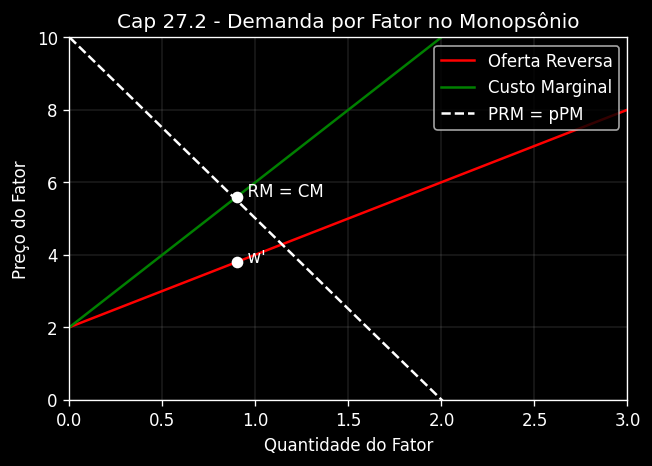
\includegraphics[scale=0.7]{cap27_2-demanda_fatores_monopsonio.png}
	\end{figure}

\end{frame}
%%%%%%%%%%%%%%%%%%%%%%%%%%%%%%%%%%%%%%%%%%%

\begin{frame}
	\frametitle{Monopólios Upstream e Downstream na Cadeia de Produção}

	Nós só observamos dois tipos de concorrência imperfeita. Mas os exemplos acima são apenas um dos múltiplos arranjos que podem acontecer na realidade.
	\\~\\
	O importante é saber como modelar o comportamento do monopolista (ou do monopsionista) seja no mercado de fatores ou no mercado de produção.
	\\~\\
	Ainda veremos uma nova situação: O caso onde um monopolista no mercado de fatores vende para um monopolista no mercado de produção.

\end{frame}

\begin{frame}
	\frametitle{Monopólios Upstream e Downstream na Cadeia de Produção}

	O monopolista do mercado de fatores é chamado de \textbf{upstream} ou \textbf{para trás}. Ele vende o insumo $x$ ao preço $k$ e com custo marginal constante $c$. 
	\\~\\
	O monopolista do mercado de produto será denominado por \textbf{downstream} ou \textbf{para frente}. Esse segundo usará o insumo $x$ para obter a produção  $y$ via função de produção da forma $f(x) = y$ que será vendida no mercado cuja demanda inversa será $p(y)$. 
	\\~\\
	No nosso exemplo a forma funcional dessa demanda será $p(y) = a - by$.

\end{frame}

\begin{frame}
	\frametitle{Monopólios Upstream e Downstream na Cadeia de Produção}

	Vamos supor que $f(x) = y = x$, ou seja, é como se ele revendesse o produto\footnote{O que torna esse exemplo surpreendentemente válido para diversas ocasiões da vida real.}. 
	\\~\\
	Outra simplificação é que o downstream também terá custo marginal igual ao preço pago pelo insumo ($k$) ao upstream.
	\\~\\
	Teremos que buscar um equilíbrio entre os dois monopolistas. Para isso, vamos começar modelando o caso para o downstream. 

\end{frame}

\begin{frame}
	\frametitle{Monopólios Upstream e Downstream na Cadeia de Produção}

	Ele quer maximizar seu lucro que é dado pelo seguinte problema:

	\begin{center}
		\Large $\stackrel{max}{\text{\small $y$}} \ \ \stackrel{L(y)\ =\ p(y)y - ky}{\ }$ \\
		\end{center}
		\begin{center}
		\Large $\stackrel{max}{\text{\small $y$}} \ \ \stackrel{L(y)\ =\ [a - by]y - ky}{\ }$ \\
		\end{center}
		\begin{center}
		\Large $\stackrel{max}{\text{\small $y$}} \ \ \stackrel{L(y)\ =\ ay - by^2 - ky}{\ }$ \\
	\end{center}

	A condição de primeira ordem da última forma é dada por:

	$$ \frac{d L(y)}{d y} = a - 2by - k = 0 $$
	$$ a - 2by = k $$
	$$ y = \frac{a - k}{2b} $$

\end{frame}

\begin{frame}
	\frametitle{Monopólios Upstream e Downstream na Cadeia de Produção}

	Como a função de produção usada iguala a quantidade de insumo à quantidade de produto. Vemos que ele demandará exatamente a mesma quantidade de fator de produção que a oferta no mercado do produto.

	$$ y = x = \frac{a - k}{2b} $$

	O importante aqui é perceber que a função de produção do monopolista downstream é usada para derivar a demanda do fator produzido pelo upstream. 
	\\~\\
	Perceba que a quantidade demandada de fator depende do preço pago por ele e da demanda no mercado de produto. Tudo bem intuitivo e simples.

\end{frame}

\begin{frame}
	\frametitle{Monopólios Upstream e Downstream na Cadeia de Produção}

	Agora temos que modelar o comportamento do upstream. Vamos supor que ele tenha acesso à função demanda de fatores do downstream e queira maximizar seu lucro.

	A demanda inversa de fatores nada mais é do que a última equação tendo k em função de x:

	$$ k(x) = a - 2bx $$

	A receita é dada por:

	$$ k(x)x = ax - 2bx^2 $$

	E a receita marginal por:

	$$ RM_x = a - 4bx $$

\end{frame}

\begin{frame}
	\frametitle{Monopólios Upstream e Downstream na Cadeia de Produção}

	Igualando a receita marginal ao custo marginal, teremos que:

	$$ a - 4bx = c $$

	ou seja, o total vendido no mercado pelo monopolista upstream será dado por:

	$$ x = \frac{a - c}{4b} $$

	Como a função de produção é um pra um, podemos definir que o total produzido no mercado de produto será:

	$$ y = \frac{a - c}{4b} $$

	Essa é a quantidade da produção que maximiza os lucros do monopolista upstream.

\end{frame}

\begin{frame}
	\frametitle{Monopólios Upstream e Downstream na Cadeia de Produção}

	Lembre-se que ele usa como função de demanda de fatores o resultado do problema de maximização do downstream. Então a solução acaba por gerar um lucro fruto do processo de maximização de ambos os monopolistas.
	\\~\\
	Se houvesse apenas um monopolista em ambos os mercados (imagine que as duas empresas se fundissem) e os custos de produção dos fatores se mantivessem os mesmos.
	\\~\\
	O problema de maximização seria igualar a receita marginal ($a - 2by$) ao custo do fator ($c$). Isso geraria um volume de produção igual à

	$$ y_{int} = \frac{a - c}{2b}$$

\end{frame}

\begin{frame}
	\frametitle{Monopólios Upstream e Downstream na Cadeia de Produção}

	O monopolista integrado produzirá o dobro que o arranjo com dois monopolistas separados. Mas qual o motivo dessa diferença?
	\\~\\
	Na prática, o monopolista upstream vai cobrar uma quantidade cujo preço de mercado é superior ao custo marginal. 
	\\~\\
	Esse preço será o custo que o monopolista downstream usará para maximizar seu lucro. 
	\\~\\
	Contudo, quando as empresas se fundem, o novo custo marginal do monopolista do mercado de produto será exatamente o custo de produção $c$. Nós retiramos de cena o Markup do monopolista upstream.

\end{frame}

%%%%%%%%%%%%%%%%%%%%%%%%%%%%%%%%%%%%%%%%%%%
\section{Oligopólio}
%%%%%%%%%%%%%%%%%%%%%%%%%%%%%%%%%%%%%%%%%%%

\begin{frame}
	\huge O Oligopólio \normalsize
	\\~\\
	\begin{itemize}
		\item A Escolha de uma Estratégia
		\item Liderança na Quantidade
		\item Liderança no Preços
		\item Estabelecimento Simultâneo da quantidade (Equilíbrio de Cournot)
		\item Ajustamento para o Equilíbrio
		\item Várias Empresas no Equilíbrio de Cournot
		\item Fixação Simultânea de Preços
		\item Conluio
		\item Estratégias Punitivas
		\item Comparação das Soluções
	\end{itemize}
\end{frame}

\begin{frame}
	\frametitle{O Oligopólio}

	Pensemos em uma situação onde temos poucos concorrentes.
	\\~\\
	De um lado, não temos tantos a ponto de ninguém poder manipular seus preços.
	\\~\\
	Do outro, ninguém é grande o suficiente para ignorar o comportamento dos seus concorrentes. 
	\\~\\
	Esse arranjo é denominado de \textbf{Oligopólio}.
	\\~\\
	Vamos partir da estrutura de competição de apenas duas empresas: o \textbf{Duopólio}. Outra limitação que imporemos é a de que os produtos são idênticos.
	\\~\\
	Nosso foco são as \textbf{interações estratégicas}.

\end{frame}

\begin{frame}
	\frametitle{A Escolha de uma Estratégia}

	Em um arranjo de dois competidores, temos que desenvolver um modelo que consiga equilibrar 4 variáveis:

	\begin{itemize}
		\item Preço da Empresa 1
		\item Preço da Empresa 2
		\item Quantidade da Empresa 1
		\item Quantidade da Empresa 2
	\end{itemize}
	\ 
	\\~\\
	Quando as duas empresas decidem sem ter acesso a informação do adversário, elas precisam supor o que ele fará. Esse arranjo é denominado \textbf{jogo simultâneo}.

\end{frame}

\begin{frame}
	\frametitle{A Escolha de uma Estratégia}

	Chamaremos de \textbf{líder} toda empresa que decidir seu \textbf{preço} ou \textbf{quantidade} antes da outra. 
	\\~\\
	A empresa que decidirá após a informação da decisão da empresa líder será chamada de \textbf{seguidora}. 
	\\~\\
	As interações desse tipo são chamadas de \textbf{jogos sequenciais}.

\end{frame}


\begin{frame}
	\frametitle{A Escolha de uma Estratégia}

	Com esses dois conceitos, podemos ter 4 tipos de interações estratégicas:

	\begin{itemize}
		\item Liderança de Preço
		\item Liderança de Quantidade
		\item Preço Simultâneo
		\item Quantidade Simultânea
	\end{itemize}
	\ 
	\\~\\
	Além dessas, veremos uma opção possível de estratégia onde há negociação entre as empresas para formação de um \textbf{conluio}. Esse tipo de esquema é chamado de \textbf{jogo cooperativo}.

\end{frame}

\begin{frame}
	\frametitle{Liderança na Quantidade}

	O modelo desenvolvido nessa seção é creditado ao economista alemão Heinrich von Stackelberg. Seu livro \textit{Marktform und Gleichgewicht} foi publicado em 1934.
	\\~\\
	Vamos supor que temos uma empresa líder na quantidade. Ela fixará sua produção em $y_1$ unidades.
	\\~\\
	A empresa seguidora, de posse da informação de $y_1$ e da demanda inversa do mercado, escolherá seu nível de produção em $y_2$.
	\\~\\
	A demanda inversa do mercado será em função do total de produtos $p(Y) = p(y_1 + y_2)$.

\end{frame}

\begin{frame}
	\frametitle{Liderança na Quantidade}

	Como a empresa líder decidirá sua quantidade de modo a maximizar seus lucros?
	\\~\\
	Não seria nada estranho que ela tivesse a hipótese que a empresa seguidora queira maximizar seus lucros também.
	\\~\\
	Desse modo, a empresa líder terá que endogenizar o problema da maximização do lucro da empresa seguidora.
	\\~\\
	O problema da maximização da empresa seguidora é:

	\begin{center}
	\LARGE $\stackrel{max}{\text{\small $y_2$}} \ \ \stackrel{p(y_1 + y_2)y_2 - c_2(y_2)}{\ }$ \\
	\end{center}

\end{frame}

\begin{frame}
	\frametitle{Liderança na Quantidade}

	Queremos encontrar o ponto onde a receita marginal será igual ao custo marginal.

	$$ RM_2 = CMa_2 = p(y_1 + y_2) + \frac{dp(y_1+y_2)}{dy_2}y_2 - \frac{dc_2(y_2)}{y_2} = 0 $$

	A novidade aqui é que temos que levar em consideração a quantidade $y_1$ para encontrar nosso $y_2$. Isso quer dizer que 

	$$y_2 = f_2(y_1)$$

\end{frame}

\begin{frame}
	\frametitle{Liderança na Quantidade}

	Nós conseguimos obter essa função isolando nosso termo $y_2$ no problema de maximização acima.
	\\~\\
	Essa função tem o nome de \textbf{função de reação} e nos diz qual quantidade será produzida pela empresa seguidora ao ser conhecida a quantidade da empresa líder.
	\\~\\
	Vamos definir a função de demanda inversa como $p(y_1 + y_2) = a - b(y_1 + y_2)$ e também adotaremos o custo igual a zero para facilitar a matemática da coisa.

\end{frame}

\begin{frame}
	\frametitle{Liderança na Quantidade}

	$$\textrm{Função Lucro 2: } \pi_2(y_1,y_2) = p(y_1 + y_2)y_2$$
	
	$$ = [a - b(y_1 + y_2)]y_2 = ay_2 - by_1 y_2 - by_2^2 $$

	Com a função de lucro e a de reação, conseguimos ver a relação entre essas duas funções. 
	\\~\\
	Na imagem abaixo podemos ver que a curva de reação sempre atravessa as curvas de isolucro no ponto onde temos o maior valor de $y_2$.

\end{frame}

\begin{frame}
	\frametitle{Liderança na Quantidade}

	\begin{figure}[H]
		\centering
		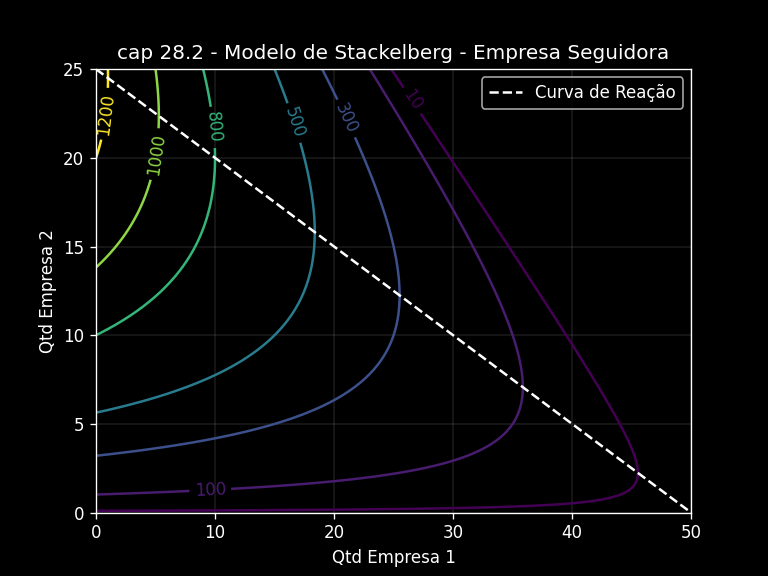
\includegraphics[scale=0.55]{cap28_2-modelo_stackelberg_parcial.png}
	\end{figure}
	
\end{frame}

\begin{frame}
	\frametitle{Liderança na Quantidade}

	Agora vamos desenvolver como essa empresa define a sua quantidade de modo a maximizar o seu lucro.
	\\~\\
	Uma das características desse modelo é que a empresa líder conhece $f_2(y_1)$.

	\begin{center}
		\LARGE $\stackrel{max}{\text{\small $y_1$}} \ \ \stackrel{p(y_1 + y_2)y_1 - c_1(y_1)}{\ }$ \\
		\small de modo que \normalsize $y_2 = f_2(y_1)$
	\end{center}

	Ou melhor

	\begin{center}
		\LARGE $\stackrel{max}{\text{\small $y_1$}} \ \ \stackrel{p[y_1 + f_2(y_1)]y_1 - c_1(y_1)}{\ }$ \\
	\end{center}
		
\end{frame}

\begin{frame}
	\frametitle{Liderança na Quantidade}

	A produção total será definida pela líder sendo que será parte devida a produção direta e a outra parte pela resposta da seguidora ao nível definido da produção, ou seja, $y_1 + f_2(y_1)$.
	\\~\\
	Pela equação da demanda inversa linear, temos que a função de reação da empresa seguidora é

	$$ f_2(y_1) = y_2 = \frac{a - by_1}{2b}$$

	A função lucro é dada pela receita menos os custos (que no nosso exemplo é zero)

	$$ \textrm{Função Lucro 1: } \pi(y_1,y_2) = [a - b(y_1 + y_2)]y_1 = ay_1 -by_1^2 - by_1y_2 $$

\end{frame}

\begin{frame}
	\frametitle{Liderança na Quantidade}

	Colocando a função de reação dentro da função de lucro teremos

	$$ = ay_1 -by_1^2 - by_1f(y_1)$$
	$$ = ay_1 -by_1^2 - by_1\frac{a - by_1}{2b}$$
	$$ = ay_1 -by_1^2 - \frac{\cancel{b}y_1a}{2\cancel{b}} + \frac{\cancel{b}*b(y_1)^2}{2\cancel{b}}$$
	$$= ay_1 -by_1^2 - \frac{ay_1}{2} + \frac{by_1^2}{2}$$
	$$ \pi(y_1,y_2) = \frac{a}{2}y_1 - \frac{b}{2}y_1^2$$

\end{frame}

\begin{frame}
	\frametitle{Liderança na Quantidade}

	Para encontrarmos a quantidade ótima basta derivar a função lucro em função de $y_1$ e igualar a zero. O que nos dará 

	$$ y_1^* = \frac{a}{2b} $$

	Desse modo, podemos encontrar facilmente a produção de equilíbrio da empresa seguidora.

	$$ y_2^* = \frac{a - by_1}{2b} $$
	$$ y_2^* = \frac{a - b(a/2b)}{2b} $$
	$$ y_2^* = \frac{a}{4b} $$

\end{frame}

\begin{frame}
	\frametitle{Liderança na Quantidade}

	Por fim, podemos ter a quantidade total do mercado pela soma de $y_1^* + y_2^* = \frac{3a}{4b}$. 
	\\~\\
	O ponto de Equilíbrio de Stackelberg acontecerá onde \textbf{a curva de reação tangencia a maior curva de isolucro} da empresa líder. 
	\\~\\
	No exemplo da imagem eu usei para a função da demanda inversa linear um $a = 100$ e um $b = 2$.
	\\~\\
	Agora que temos a função de lucro da empresa 1, podemos acrescentar as curvas de isolucro para vermos a solução gráfica da álgebra que acabamos de desenvolver.

\end{frame}

\begin{frame}
	\frametitle{Liderança na Quantidade}

	\begin{figure}[H]
		\centering
		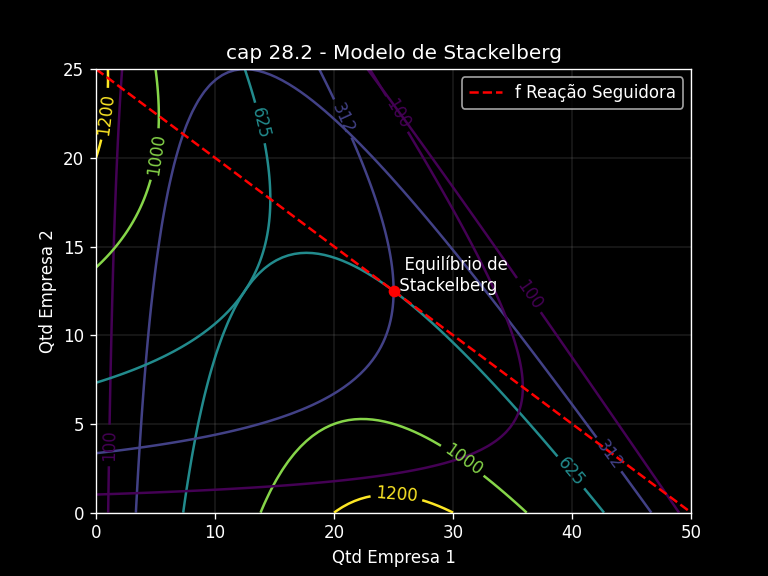
\includegraphics[scale=0.55]{cap28_2-modelo_stackelberg_completo.png}
	\end{figure}

\end{frame}

\begin{frame}
	\frametitle{Liderança no Preços}

	Outra forma de um jogo sequencial acontecer entre duas empresas é pela definição do preço pela empresa líder. 
	\\~\\
	Similarmente ao que vimos na seção anterior, a empresa líder precisa levar em consideração o que a empresa seguidora fará.
	\\~\\
	A seguidora recebe o preço definido pela líder e maximiza seu lucro.

	\begin{center}
		\LARGE $\stackrel{max}{\text{\small $y_2$}} \ \ \stackrel{py_2 - c_2(y_2)}{\ }$ \\
	\end{center}

\end{frame}

\begin{frame}
	\frametitle{Liderança no Preços}

	A empresa líder, sabendo a função de oferta da empresa seguidora, vai trabalhar com a diferença entre a Demanda do mercado e a demanda da empresa seguidora, ou seja, $R(p) = D(p) - S(p)$. 
	\\~\\
	O nome dessa curva de demanda reduzida é \textbf{curva de demanda residual}.
	\\~\\
	Supondo um custo de produção constante $c$. A função de lucro da empresa líder é dada por

	$$ \textrm{Função Lucro 1: } \pi_1(p) = R(p)p - R(p)c = (p - c)R(p) $$

\end{frame}

\begin{frame}
	\frametitle{Liderança no Preços}

	A maximização dessa empresa acontece onde a receita marginal (que nesse caso é oriunda da demanda residual) é igual ao custo marginal.
	\\~\\
	Definindo nossa demanda como $D(p) = a - bp$ e as funções custo para a seguidora $c_2(y_2) = y_2^2/2$ e para a líder $c_1(y_1) = cy_1$.
	\\~\\
	Isso nos diz que a condição de maximização da empresa seguidora será a derivada da função lucro igual a zero.

	$$ \frac{d L(y_2)}{y_2} = p - \frac{2y_2}{2} = 0 $$
	$$ = p - y_2 = 0 $$
	$$ = p = y_2 $$

\end{frame}

\begin{frame}
	\frametitle{Liderança no Preços}

	Nossa função de oferta da seguidora será $S(p) = p$. 
	\\~\\
	De posse dessa informação, podemos descobrir a equação da demanda residual da empresa líder pela subtração da curva de demanda pela oferta da seguidora.

	$$ R(p) = D(p) - S(p) = a - bp - p = a - (b + 1)p $$

	Agora é só maximizar o lucro pela igualdade entre a receita marginal e o custo marginal e verificar na curva de demanda inversa o volume de produção e o preço.

\end{frame}

\begin{frame}
	\frametitle{Liderança no Preços}

	Demanda inversa é obtida isolando $p$ da demanda residual.

	$$ p(y_1) = \frac{a}{b+1}-\frac{1}{b+1}y_1 $$

	A receita da empresa líder é obtida pela multiplicação de $p(y_1)$ por $y_1$. A receita marginal é a derivada dessa função em relação a $y_1$.

	$$ Receita_1: \left[ \frac{a}{b+1} - \frac{1}{b+1}y_1 \right] y_1 $$
	$$ = \frac{a}{b+1}y_1 - \frac{1}{b+1}y_1^2 $$

	A receita marginal será

	$$ RMa_1 = \frac{a}{b+1} - \frac{2}{b+1}y_1 $$

\end{frame}

\begin{frame}
	\frametitle{Liderança no Preços}

	O nosso custo foi definido como $c_1(y_1) = cy_1$, logo, o custo marginal é igual a $c$.
	\\~\\
	Portanto, nosso problema de maximização será dado pela equação

	$$ \frac{a}{b+1} - \frac{2}{b+1}y_1 = c $$
	$$ y_1^* = \frac{c(b+1)}{2} $$

	Na imagem, nós podemos ver as variáveis interagindo. A oferta total será a soma das quantidades de ambas empresas. Por acaso, a oferta da seguidora está igual à receita marginal da líder mas isso é só um acaso.

\end{frame}

\begin{frame}
	\frametitle{Liderança no Preços}

	\begin{figure}[H]
		\centering
		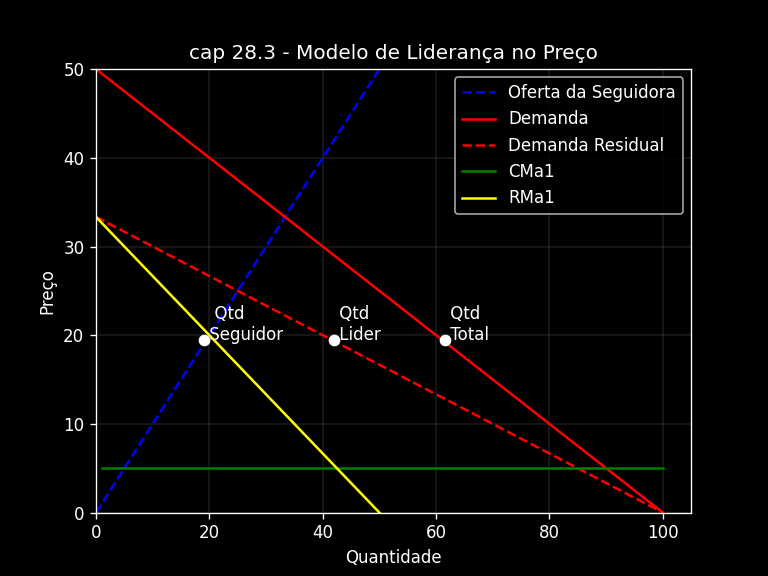
\includegraphics[scale=0.55]{cap28_3-lideranca_preco.png}
	\end{figure}

\end{frame}

\begin{frame}
	\frametitle{Estabelecimento Simultâneo da quantidade}

	Não é comum que as empresas fiquem se comunicando para informar seus concorrentes a respeito de suas decisões.
	\\~\\
	Nesses cenários, as empresas precisam supor o que suas concorrentes farão.
	\\~\\
	Esse modelo é chamado de \textbf{Modelo de Cournot} e é um modelo de jogo simultâneo onde as empresas definem suas quantidades produzidas e vendidas no mercado.
	\\~\\
	Suporemos que as empresas queiram maximizar seus lucros.

\end{frame}

\begin{frame}
	\frametitle{Estabelecimento Simultâneo da quantidade}

	A quantidade total do mercado será dada por $Y = y_1 + y_2^e$, onde $y_2^e$ é a quantidade prevista da empresa 2. 
	\\~\\
	O preço de equilíbrio do mercado será dado pela equação de demanda inversa $p(Y) = p(y_1 + y_2^e)$.
	\\~\\
	O problema de maximização do lucro será

	\begin{center}
		\LARGE $\stackrel{max}{\text{\small $y_1$}} \ \ \stackrel{p(y_1 + y_2^e)y_1 - c(y_1)}{\ }$ \\
	\end{center}

\end{frame}

\begin{frame}
	\frametitle{Estabelecimento Simultâneo da quantidade}

	Existe uma relação entre essa expectativa e a produção, de modo mais formal, $y_1 = f(y_2^e)$.
	\\~\\
	Essa é a \textbf{curva de reação} da empresa, a diferença é que aqui a empresa 1 não é mais a líder e essa reação se refere a \textit{expectativa} da produção. Mas o tratamento matemático é o mesmo.
	\\~\\
	Similarmente, a empresa 2 se depara com a mesma situação.

	$$y_2 = f(y_1^e)$$

\end{frame}

\begin{frame}
	\frametitle{Estabelecimento Simultâneo da quantidade}

	O equilíbrio de Cournot é dado pelo sistemas de equações

	$$ y_1^* = f_1(y_2^*) $$
	$$ y_2^* = f_2(y_1^*) $$

	Nenhuma das empresas terá incentivos em mudar seu nível de produção.
	\\~\\
	Se reutilizarmos o exemplo na liderança da quantidade (com custo zero e demanda linear) obteremos as mesmas funções de reação que a empresa 2 tinha naquele modelo.

\end{frame}

\begin{frame}
	\frametitle{Estabelecimento Simultâneo da quantidade}

	$$ y_1 = \frac{a - by_2^e}{2b} $$

	e

	$$ y_2 = \frac{a - by_1^e}{2b} $$

	O ponto de equilíbrio acontece onde $y_1 = y_2$, ou seja, onde as curvas de reação são iguais. Nesse ponto, $y_1^e = y_1$ e $y_2^e = y_2$. 
	\\~\\
	Só precisamos substituir dentro desse sistema de equações do seguinte modo

\end{frame}

\begin{frame}
	\frametitle{Estabelecimento Simultâneo da quantidade}

	$$ y_1 = \frac{a - by_2^e}{2b} $$
	$$ y_1 = \frac{a - by_2}{2b} $$
	$$ y_1 = \frac{a - b(\frac{a - by_1}{2b})}{2b} $$
	$$ y_1^* = \frac{a}{3b} = y_2^* $$

	Com essas funções e as equações de lucro podemos ver graficamente o equilíbrio de Cournot onde as curvas de reação se equivalem.

\end{frame}

\begin{frame}
	\frametitle{Estabelecimento Simultâneo da quantidade}

	\begin{figure}[H]
		\centering
		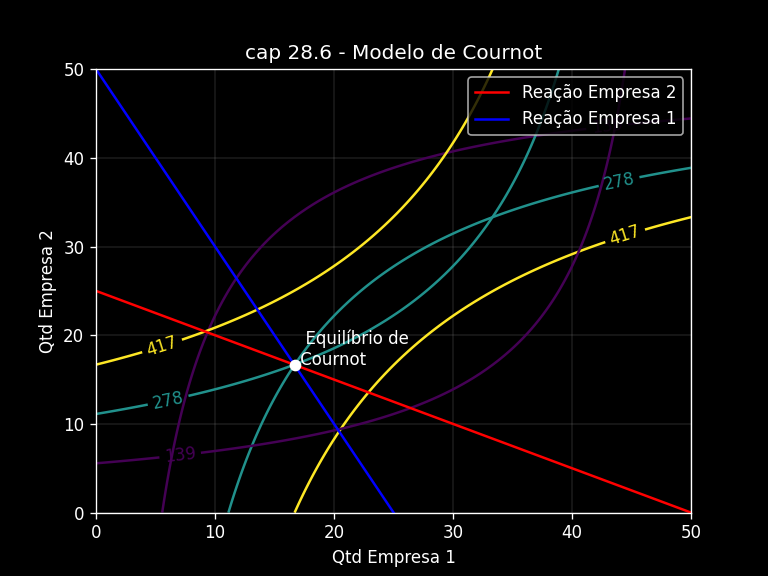
\includegraphics[scale=0.55]{cap28_6-modelo_cournot.png}
	\end{figure}
	
\end{frame}

\begin{frame}
	\frametitle{Ajustamento para o Equilíbrio}

	Seria muita boa vontade supor que, na vida real, as empresas conseguissem acertar na mosca o nível de produção dos seus concorrentes. 
	\\~\\
	Mas o nosso modelo é forte o suficiente para um processo de ajustamento em caso de (prováveis) palpites equivocados no nível de produção.
	\\~\\
	Vamos supor que a cesta inicial produzida esteja em cima da curva de reação da empresa 2. A cesta inicial, que chamamos no gráfico de $Cesta(t)$ será igual à lista $(y_1^t,y_2^t)$.
	\\~\\
	Essa cesta está na curva de reação da empresa 2, logo, essa empresa não terá incentivo a fazer nenhuma mudança. Mas para a empresa 1, a situação é outra, ela quer reduzir sua produção para aumentar seus lucros.

\end{frame}

\begin{frame}
	\frametitle{Ajustamento para o Equilíbrio}

	\begin{figure}[H]
		\centering
		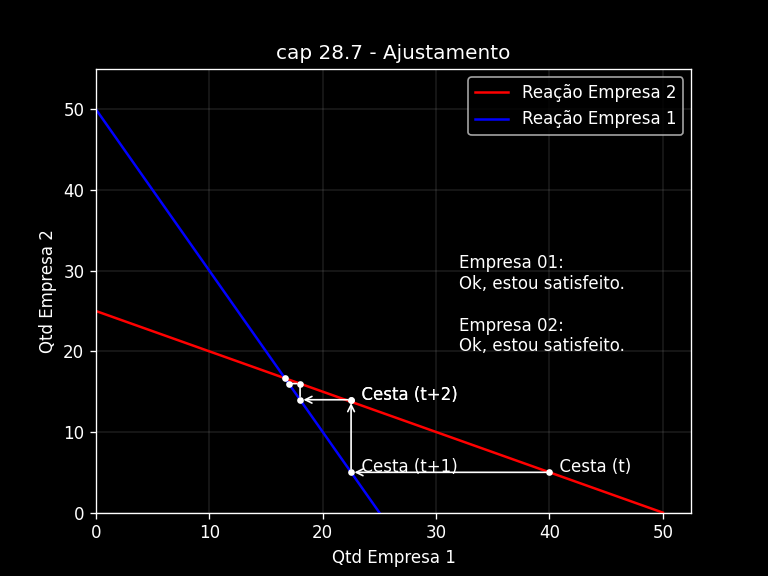
\includegraphics[scale=0.55]{cap28_7-ajustamento.png}
	\end{figure}

\end{frame}


\begin{frame}
	\frametitle{Várias Empresas no Equilíbrio de Cournot}

	A oferta total da indústria será dada por $Y = y_1 + y_2 + \dots + y_{n-1} + y_n$. Desse modo o problema da maximização da empresa será dado pela igualdade entre a receita marginal e o seu custo marginal do seguinte modo

	$$ p(Y) + \frac{\delta p}{\delta Y} y_i = CMa(y_i) $$
	$$ p(Y) + \frac{\delta p}{\delta Y} \frac{Y}{Y} \frac{p(Y)}{p(Y)} y_i = CMa(y_i) $$
	$$ p(Y) \left[1 + \frac{\delta p}{\delta Y} \frac{Y}{p(Y)} \frac{y_i}{Y} \right] = CMa(y_i) $$

\end{frame}

\begin{frame}
	\frametitle{Várias Empresas no Equilíbrio de Cournot}

	Definindo $s_i = \frac{y_i}{Y}$ como a participação da empresa no total do mercado.

	$$ p(Y) \left[1 + \frac{\delta p}{\delta Y} \frac{Y}{p(Y)} s_i \right] = CMa(y_i) $$

	Se lembrarmos da fórmula da elasticidade, podemos ver que o termo $\frac{\delta p}{\delta Y} \frac{Y}{p(y)}$ é justamente o inverso da elasticidade $\frac{1}{\epsilon(Y)}$

	$$ p(Y) \left[1 - \frac{s_i}{|\epsilon(Y)|} \right] = CMa(y_i) $$

	Que é o mesmo que

	$$ p(Y) \left[1 - 1/\frac{|\epsilon(Y)|}{s_i} \right] = CMa(y_i) $$

\end{frame}

\begin{frame}
	\frametitle{Várias Empresas no Equilíbrio de Cournot}

	Essa solução é bem parecida com a maximização do monopolista. 
	\\~\\
	A principal diferença é esse termo $s_i$ dividindo a elasticidade. 
	\\~\\
	Como $s_i = y_i/Y$ ele será $0 \leq s_i \leq 1$. 
	\\~\\
	No caso monopolista, sabemos que $s_i = 1$. No outro extremo, se $lim (s_i) \rightarrow 0$, a empresa terá elasticidade infinita como as empresas da competição perfeita.
	\\~\\
	Quanto maior $s_i$ menor será a elasticidade da demanda da empresa.
\end{frame}

\begin{frame}
	\frametitle{Fixação Simultânea de Preços}

	Em algum momento do século XIX, um matemático francês de nome Joseph Bertrand, ao ler o livro do Cournot, desenvolveu um modelo simultâneo de equilíbrio de preços. 
	\\~\\
	Esse modelo ficou conhecido como \textbf{concorrência de Bertrand}.

\end{frame}

\begin{frame}
	\frametitle{Fixação Simultânea de Preços}

	Estamos na busca do par de preços que permitam ambas as empresas maximizar seus lucros. Para isso, temos que seguir algumas regras vindas dos modelos de maximização já vistos até agora:

	\begin{itemize}
		\item O preço não poderá ser maior que o custo marginal porque as empresas aumentariam seus lucros simplesmente produzindo menos.
		\item Se o preço for maior que o custo marginal, todas as empresas terão um incentivo de reduzir seu preço para "roubar"\ os clientes das concorrentes e ainda auferir lucros positivos.
	\end{itemize}
	
\end{frame}

\begin{frame}
	\frametitle{Fixação Simultânea de Preços}

	O segundo ponto funciona de maneira recursiva. 
	\\~\\
	Se uma empresa reduz seu preço em $10\%$ abaixo dos preços das suas concorrentes, ela ganhará parte do mercado. 
	\\~\\
	As concorrentes terão o incentivo em reduzir mais ainda seus preços até o ponto onde não poderão mais reduzir (determinado pelo custo marginal).
	\\~\\
	O ponto onde não será possível reduzir os preços é justamento a igualdade do custo marginal. Que é a imposição 1 do nosso modelo. Esse é precisamente o equilíbrio de Bertrand.

\end{frame}

\begin{frame}
	\frametitle{Conluio}

	Todas as soluções envolveram processos de competição entre as empresas.
	\\~\\
	Não seria nem um pouco alheio à realidade supor que algumas empresas queiram operar de modo coordenado. 
	\\~\\
	Esse arranjo é chamado de \textbf{Cartel} e é crime em vários países.
	\\~\\
	Um cartel não passa de um grupo de empresas se comportando como um monopolista. 
	\\~\\
	Diante disso, seu problema de maximização será muito parecido com o modelo do capítulo que tratamos sobre o monopólio.

\end{frame}

\begin{frame}
	\frametitle{Conluio}

	O problema da maximização para um cartel de duas empresas será dado por

	\begin{center}
		\LARGE $\stackrel{max}{\text{\small $y_1,y_2$}} \ \ \stackrel{p(y_1+y_2)[y_1 + y_2] - c_1(y_1) - c_2(y_2)}{\ }$ \\
	\end{center}

	Cujas condições de primeira ordem serão

	$$p(y_1^* + y_2^*) + \frac{\delta p}{\delta Y}[y_1^* + y_2^*] = CMa_1(y_1^*)$$
	$$p(y_1^* + y_2^*) + \frac{\delta p}{\delta Y}[y_1^* + y_2^*] = CMa_2(y_2^*)$$

\end{frame}

\begin{frame}
	\frametitle{Conluio}

	Podemos ver que, quando uma empresa decide expandir sua produção, receberá uma quantia oriunda da venda dos seus produtos, contudo, essa oferta adicional reduzirá o preço de equilíbrio do mercado (o que reduz o lucro recebido). 
	\\~\\
	A novidade aqui é que essa redução do preço impactará também na outra empresa do cartel.
	\\~\\
	O que as duas equações anteriores nos dizem é que as quantidades produzidas (e ofertadas no mercado) serão as que igualem seus custos marginais $CMa_1(y_1^*) = CMa_2(y_2^*)$. 

\end{frame}

\begin{frame}
	\frametitle{Conluio}

	Será que as empresas que operam em um cartel possuem algum incentivo em "trapacear"\ a sua empresa parceira?
	\\~\\
	Vejamos o que acontece com a empresa 1 do nosso cartel, caso ela aumente a sua produção em $\delta y_1$ unidades. Podemos mensurar esse impacto pela derivada parcial da função lucro do cartel em relação a $y_1$

	$$ \frac{\partial \pi_1}{\partial y_1} = p(y_1^* + y_2^*) + \frac{\delta p}{\delta Y}y_1^* - CMa_1(y_1^*) $$ 

	A condição de maximização do cartel nos diz que

	$$ p(y_1^* + y_2^*) + \frac{\delta p}{\delta Y}y_1^* + \frac{\delta p}{\delta Y}y_2^* - CMa_1(y_1^*) = 0 $$ 

\end{frame}

\begin{frame}
	\frametitle{Conluio}

	Apenas isolando o termo referente à produção da empresa, temos então

	$$ p(y_1^* + y_2^*) + \frac{\delta p}{\delta Y}y_1^* - CMa_1(y_1^*) = - \frac{\delta p}{\delta Y}y_2^* $$ 

	Como $\delta p / \delta Y$ é negativo, então o termo da esquerda da última equação é positivo. Ou seja, a empresa 1 consegue aumentar seus lucros positivamente ao aumentar sua produção para além do ponto de equilíbrio do cartel.
	\\~\\
	Na solução de maximização do lucro conjunto, existe um incentivo para cada empresa aumentar sua produção, visto que, se a outra empresa mantiver fixa a sua produção, sempre será lucrativo um aumento unilateral da quantidade produzida.

\end{frame}

\begin{frame}
	\frametitle{Conluio}

	\begin{figure}[H]
		\centering
		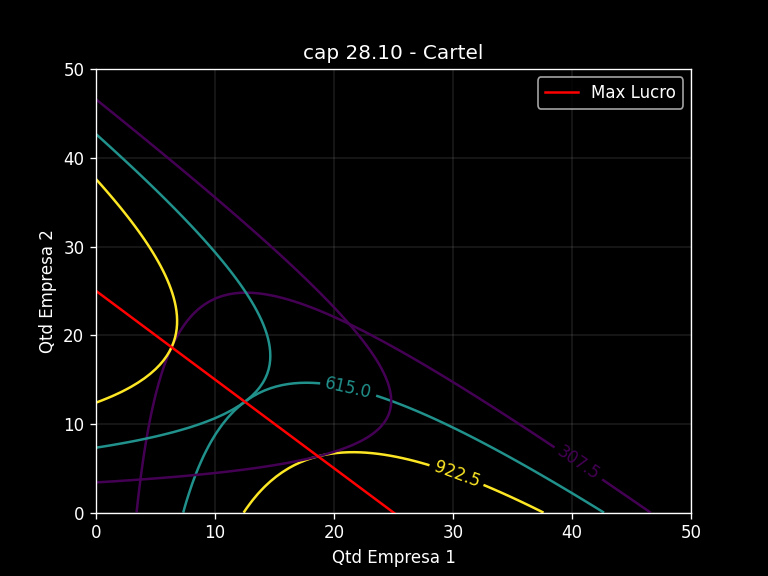
\includegraphics[scale=0.55]{cap28_10-cartel.png}
	\end{figure}

\end{frame}


\begin{frame}
	\frametitle{Estratégias Punitivas}

	Nessa parte do capítulo temos uma modelagem quanto a uma possível solução para o incentivo à trapaça dos carteis.
	\\~\\
	Mas logo após essa aula, vamos ver um ferramental melhor para analisar esse tipo de questão: A (famosa) Teoria dos Jogos.
	\\~\\
	Ainda é recomendada a leitura do material. Mas por hoje, já está bom.

\end{frame}

%%%%%%%%%%%%%%%%%%%%%%%%%%%%%%%%%%%%%%%%%%%
\section[T.Jogos]{Teoria dos Jogos}
%%%%%%%%%%%%%%%%%%%%%%%%%%%%%%%%%%%%%%%%%%%
\begin{frame}
	\huge Teoria dos Jogos \normalsize
	\\~\\
	\begin{itemize}
		\item A Matriz de Ganhos
		\item Equilíbrio de Nash
		\item Estratégias Mistas
		\item O Dilema do Prisioneiro
		\item Jogos Repetidos
		\item Manutenção de um Cartel
		\item Jogos sequenciais
		\item Barreiras à Entrada
	\end{itemize}
\end{frame}

% https://comp.text.tex.narkive.com/HHAjcLzp/sgame-and-beamer 
% sgame not working in beamer because & means something inside a frame
\newsavebox\mybox
\begin{lrbox}{\mybox}
	\begin{game}{2}{2}[Jogador A][Jogador B]
		& $Esquerda$    & $Direita$ \\
		$Alto$  & $1,2$         & $0,1$     \\
		$Baixo$ & $2,1$         & $1,0$
	\end{game}
\end{lrbox}

\begin{frame}
	\frametitle{A Matriz de Ganhos}

	No capítulo anterior nós começamos a trabalhar os conceitos de interação estratégica entre agentes, mas agora veremos um framework mais robusto chamado \textbf{Teoria do Jogos}.
	\\~\\
	vamos manter nosso horizonte de jogadores restrito a apenas dois e limitaremos o número de estratégias a um número finito. 
	\\~\\
	Assim conseguimos representar os ganhos em uma \textbf{matriz de ganhos}.

	\begin{center}
		\usebox{\mybox}
	\end{center}

\end{frame}

\def\highlight#1{\colorbox{yellow}{#1}}
\begin{lrbox}{\mybox}
	\begin{game}{2}{2}[Jogador A][Jogador B]
		& $Esquerda$    & $Direita$ \\
		$Alto$  & $1,2$         & $0,1$       \\
		$Baixo$ & \highlight{$2,1$}         & $1,0$
	\end{game}
\end{lrbox}

\begin{frame}
	\frametitle{A Matriz de Ganhos}

	Como sabemos o que cada jogador fará?
	\\~\\
	Primeiro vamos comparar os resultados de cada interação entre as estratégias possíveis.

	\begin{center}
		\usebox{\mybox}
	\end{center}

	Como há uma lógica dominante para as escolhas de ambos os jogadores, então, nesse jogo em questão, existe o que chamamos de \textbf{estratégia dominante}.

\end{frame}

\begin{lrbox}{\mybox}
	\begin{game}{2}{2}[Jogador A][Jogador B]
		& $Esquerda$    & $Direita$ \\
		$Alto$  & $2,1$         & $0,0$       \\
		$Baixo$ & $0,0$         & $1,2$
	\end{game}
\end{lrbox}

\begin{frame}
	\frametitle{Equilíbrio de Nash}

	Existem muitas situações em que não existem estratégias dominantes e foi justamente para lidar com essas situações que o Nobel de 1994 criou (ou descobriu) o conceito que usaremos agora.
	\\~\\
	Vamos olhar o seguinte jogo

	\begin{center}
		\usebox{\mybox}
	\end{center}

\end{frame}

\begin{frame}
	\frametitle{Equilíbrio de Nash}

	Percebeu que nesse arranjo não temos nenhuma estratégia dominante? O que cada jogador fará, depende da escolha do outro jogador.
	\\~\\
	Um \textbf{equilíbrio de Nash} é criado sempre que a escolha de um jogador for \textit{ótima} dada a escolha do outro jogador.
	\\~\\
	Note que um equilíbrio de estratégia dominante também é um equilíbrio de Nash mas não necessariamente o contrário.
	\\~\\
	Uma vez que seja revelado aos participantes que eles estão nesse quadrante, nenhum deles terá o incentivo em mudar de estratégia.
	\\~\\
	É o que vemos nos quadrantes alto-esquerda e baixo-direita.

\end{frame}

\begin{lrbox}{\mybox}
	\begin{game}{2}{2}[Jogador A][Jogador B]
		& $Esquerda$    & $Direita$ \\
			$Alto$  & $0,0$         & $0,-1$       \\
			$Baixo$ & $1,0$         & $-1,3$
	\end{game}
\end{lrbox}

\begin{frame}
	\frametitle{Equilíbrio de Nash}

	Mas nem tudo são flores. O conceito do equilíbrio de Nash possui algumas dificuldades.
	\\~\\
	Como vemos no exemplo de agora, podem haver múltiplos equilíbrios de Nash em um mesmo jogo.
	\\~\\
	Outra dificuldade é que existem jogos em que não existam nenhum equilíbrio de Nash sequer. Veja o jogo abaixo

	\begin{center}
		\usebox{\mybox}
	\end{center}

\end{frame}

\begin{frame}
	\frametitle{Estratégias Mistas}

	Até agora, todos os jogos que vimos foram jogos de \textbf{estratégia pura}. Onde os jogadores definem um caminho e sempre agem do mesmo modo.
	\\~\\
	De modo mais formal, podemos usar a definição dada no livro de pós-graduação do Varian (Microeconomic Analysis, 1993).
	\\~\\
	\textbf{Equilíbrio de Nash em Estratégias Puras:} Um equilíbrio de Nash em estratégias puras é um par [das estratégias] $(r^*,c^*)$ de modo que $u_r(r^*,c^*) \geq u_r(r,c^*)$ para qualquer estratégias nas linhas $r$, e similarmente, $u_c(r^*,c^*) \geq u_c(r^*,c)$ para qualquer estratégias nas colunas $c$.

\end{frame}

\begin{frame}
	\frametitle{Estratégias Mistas}

	Podemos ampliar nossa forma de pensar e permitir que os jogadores atribuam probabilidades para cada escolha e possam mudar de estratégia ao longo do tempo.
	\\~\\
	Nesse modelo, um jogador pode ficar 50\% do tempo em uma estratégia e mudar de estratégia nos outros 50\% do tempo. Auferindo o retorno de ambas multiplicado pela probabilidade associada a ela. Esse modelo é chamado de \textbf{estratégia mista}.
	\\~\\
	O equilíbrio de Nash em estratégias mistas é o equilíbrio na \textbf{escolhas das probabilidades} de cada agente. Ou seja, ao invés de escolher entre uma ou outra, ele escolherá quantos porcento de cada estratégia será utilizado. 

\end{frame}

\begin{frame}
	\frametitle{Estratégias Mistas}

	Vamos pegar esse jogo e simular todos os retornos para cada escolha de probabilidades. 
	\\~\\
	Lembre-se que, se a probabilidade de $A$ escolher $alto$ for de $10\%$, então, $baixo$ terá obrigatoriamente de ter a probabilidade igual a $90\%$. 
	\\~\\
	Os retornos de $A$ são essa escala avermelhada enquanto os retornos de $B$ são a escala azulada.

\end{frame}

\begin{frame}
	\frametitle{Estratégias Mistas}

	\begin{figure}[H]
		\centering
		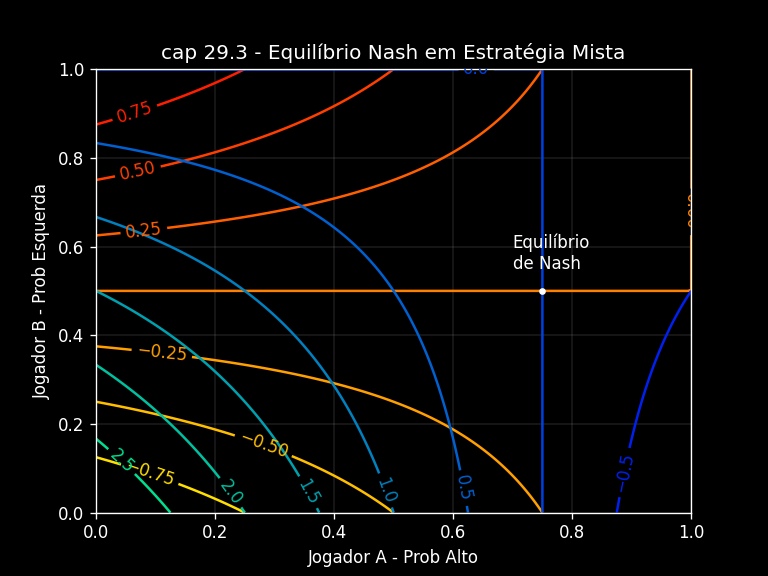
\includegraphics[scale=0.55]{cap29_3-estrategias_mistas.png}
	\end{figure}
		
\end{frame}

\begin{frame}
	\frametitle{Estratégias Mistas}

	O ponto do equilíbrio de Nash acontece onde $B$ escolhe $50\%$ para cada e $A$ escolhe $75\%$ para $alto$ e $25\%$ para $baixo$. 
	\\~\\
	Quando $B$ escolhe esse ponto, todos os retornos de $A$ se tornam constantes (veja que a linha de $A$ é uma reta horizontal nesse ponto). 
	\\~\\
	Similarmente, quando $A$ escolhe esse ponto, todos os retornos de $B$ se tornam constantes. 
	\\~\\
	Como nenhum deles tem nenhum incentivo em mudar de estratégia nesse equilíbrio, temos um equilíbrio de Nash para estratégias mistas.
	
\end{frame}

\begin{lrbox}{\mybox}
	\begin{game}{2}{2}[Jogador A][Jogador B]
		& $Confessa$      & $Nega$ \\
		$Confessa$  & $-3,-3$         & $0,-6$ \\
		$Nega$      & $-6,0$          & $-1,-1$
	\end{game}
\end{lrbox}

\begin{frame}
	\frametitle{O Dilema do Prisioneiro}

	Um dos conceitos mais conhecidos na economia é o dilema do prisioneiro.
	\\~\\
	Primeiro, considere o jogo abaixo

	\begin{center}
		\usebox{\mybox}
	\end{center}

	Esse jogo possui uma estratégia dominante: confessar. 
	\\~\\
	Independente do que cada jogador faça, sempre vai ser melhor confessar. Mas aqui temos uma contradição. Se eles optassem por não seguir a estratégia dominante, acabariam em situação melhor.

\end{frame}

\begin{frame}
	\frametitle{O Dilema do Prisioneiro}

	Como a opção "nega-nega"\ não pode ser modificada sem prejuízo para alguma das parte, ela é eficiente no sentido de Pareto. 
	\\~\\
	Ou seja, estamos diante de um arranjo que impede que alcancemos o ótimo de Pareto do sistema.
	\\~\\
	Podemos adaptar esse dilema para várias outras situações da vida real:
	\begin{itemize}
		\item "instalar"\ ou "não instalar"\ mísseis nucleares
		\item "burlar"\ ou "não burlar"\ as cotas de produção de um cartel
		\item "passar cola"\ ou "não passar cola"\ para um colega preguiçoso
	\end{itemize}

\end{frame}

\begin{frame}
	\frametitle{Jogos Repetidos}

	Como é de se esperar, o dilema do prisioneiro trouxe bastante discussão a respeito de como resolver esse jogo. 
	\\~\\
	Parece que a solução está relacionada à possibilidade ou não de repetição. Se o jogo é sem repetição, melhor será confessar. Pois essa é a estratégia dominante do arranjo.
	\\~\\
	Dentro de um jogo repetido temos dois tipos: jogos de número fixo e jogos indefinidos.
	\\~\\
	Um jogo repetido pode permitir coordenações entre os jogadores. É possível "punir"\ um jogador que decida optar por um ponto egoísta e com isso, criar o incentivo à cooperação.

\end{frame}

\begin{frame}
	\frametitle{Jogos Repetidos}

	No caso de um \textbf{jogo com repetição fixa}, é muito provável que os jogadores seguirão a estratégia dominante na última rodada, visto que não serão punidos pela outra parte.
	\\~\\
	Contudo, se você já sabe que o jogador será egoísta na última rodada, o que impede de ele repetir esse ato na penúltima, e na antepenúltima e assim por diante?
	\\~\\
	Se não houver uma garantia de cooperação na última rodada, a maior chance é que o jogo siga na estratégia dominante. 

\end{frame}

\begin{frame}
	\frametitle{Jogos Repetidos}

	Esse padrão não é mantido em um jogo indefinido. 
	\\~\\
	Como sempre haverá uma oportunidade de punir os comportamentos não cooperativos, a tendência é que os jogadores sigam para o equilíbrio de Pareto.
	\\~\\
	Robert Axelrod fez um torneio computacional com vários algoritmos de estratégias em uma simulação do dilema do prisioneiro. A estratégia que performou melhor foi a que usou o "olho por olho".

\end{frame}

\begin{frame}
	\frametitle{Manutenção de um Cartel}

	Nessa seção revisitamos o problema da manutenção do cartel, mas sob a ótica da teoria dos jogos.
	\\~\\
	Na prática, esse problema pode ser modelo em termos de um dilema do prisioneiro.
	\\~\\
	Seguir as cotas é igual ao ponto de cooperação. Vender a custo competitivo (o ponto de Bertrand) é o equivalente a confessar e, portanto, é o equivalente ao equilíbrio de Nash.
	\\~\\
	Se a parte prejudicada puder responder ao trapaceiro e depois propor a recriação do cartel, o trapaceiro pode aprender a trabalhar em equipe. Mas se o prejudicado for do tipo de pessoa que não perdoa nunca, o cartel será destinado ao ponto de competição.

\end{frame}

\begin{lrbox}{\mybox}
	\begin{game}{2}{2}[Jogador A][Jogador B]
		& $Esquerda$     & $Direita$ \\
		$Alto$      & $1,9$          & $1,9$ \\
		$Baixo$     & $0,0$          & $2,1$
	\end{game}
\end{lrbox}

\begin{frame}
	\frametitle{Jogos sequenciais}

	O modelo de Stackelberg é um exemplo de um jogo onde as ações são alternadas entre os jogadores. Nesses casos, além da matriz de ganhos, nós podemos usar a \textbf{forma extensiva do jogo} para ilustrar as etapas de escolhas e os devidos retornos de cada uma delas.
	\\~\\
	Observe o jogo abaixo

	\begin{center}
		\usebox{\mybox}
	\end{center}

	Se pensarmos nesse jogos como um jogo sequencial onde $A$ toma a primeira ação, podemos demonstrar o processo de decisão por meio do diagrama de árvore abaixo

\end{frame}

\begin{frame}
	\frametitle{Jogos sequenciais}

	\Tree[.\textit{Jogador A} 
	[.Alto 
		[.\textit{Jogador B}
			[.Esquerda (1,9) ]
			[.Direita (1,9) ]]]
	[.Baixo 
		[.\textit{Jogador B}
			[.Esquerda (0,0) ]
			[.Direita (2,1) ]]]]
	\\
	\ 
	\\
	O jogador $A$ tem como estratégia escolher $baixo$, pois assim, terá o retorno de $2$ ao invés de $1$. O jogador $B$ só tem a opção de escolher dentro das opções de $baixo$, o que lhe sobra é a opção $direita$.

\end{frame}

\begin{frame}
	\frametitle{Jogos sequenciais}

	Mas $B$ poderia pensar em manerias de obrigar o jogador $A$ a escolher $alto$.
	\\~\\
	Se $B$ ameaçar uma retaliação e escolher $esquerda$, ambos terminariam com $0$. Contudo, $A$ só levaria a sério essa ameaça se houvesse forte indício de cumprimento.
	\\~\\
	Se $B$ conseguir limitar seu escopo de atuação, é possível que a estratégia de $A$ seja modificada porque a matriz de ganhos seria modificada também.
	\\~\\
	Se você está acompanhando os noticiários, pode ver claramente como Putin tenta colocar nos outros a responsabilidade por uma possível escalada da guerra. Ele afirma que será "obrigado"\ a aumentar a força se ajudarem a Ucrânia.
\end{frame}

\begin{frame}
	\frametitle{Barreiras à Entrada}

	Voltemos no problema da entrada de concorrentes em um mercado monopolizado.
	\\~\\
	Nós vimos que o monopolista possui o poder de retalhar devido a escala mínima de eficiência (EME) e do controle do mercado.
	\\~\\
	Quando uma empresa pondera em entrar no mercado, ela precisa contar com as possíveis consequências por conta do monopolista e, da mesma maneira, o monopolista precisa ponderar se valerá a pena baixar os preços para evitar o concorrente.
\end{frame}

\begin{lrbox}{\mybox}
	\begin{game}{2}{2}[Entrante][Monopolista]
		& $Retalha$      & $\textrm{Não Retalha}$ \\
		$Entra$               & $0,0$          & $2,1$ \\
		$\textrm{Fica Fora}$  & $1,9$          & $1,9$
	\end{game}
\end{lrbox}

\begin{frame}
	\frametitle{Barreiras à Entrada}

	Podemos exemplificar essa questão com a matriz abaixo

	\begin{center}
		\usebox{\mybox}
	\end{center}

	A primeira vista, temos dois equilíbrios de Nash. Mas esse também é um exemplo de um jogo sequenciado. Quem tem o poder de liderança é a empresa entrante.
	\\~\\
	Vamos olhar como fica esse problema no diagrama de árvore.

\end{frame}

\begin{frame}
	\frametitle{Barreiras à Entrada}

	\Tree[.\textit{Entrante} 
				[.\textit{Fica Fora} 
					[.\textit{Monopolista}
						[.Retalha (1,9) ]
						[.\textit{Não Retalha} (1,9) ]]]
				[.Entra
					[.\textit{Monopolista}
						[.Retalha (0,0) ]
						[.\textit{Não Retalha} (2,1) ]]]]
	\\
	\ 
	\\
	A condição de entrada ou não é baseada na promessa de haver ou não retalhação.
	\\~\\
	A estratégia da entrante é optar por concorrer no mercado.

\end{frame}

\begin{frame}
	\frametitle{Barreiras à Entrada}

	O que o monopolista fará? Bom, não existe maneira garantida do monopolista vincular a entrada do novo concorrente com a retaliação. 
	\\~\\
	Uma vez que o novo competidor se instalou, não é racional baixar os preços e abrir mão do lucro.
	\\~\\
	Agora, se o monopolista conseguir modificar sua matriz de ganhos (por meio de investimento na capacidade produtiva) de modo a obter lucro mesmo na retalhação, o cenário será outro.
	\\~\\
	Seria mais compensador ao monopolista lutar pelo seu mercado do que se acovardar.
\end{frame}

%%%%%%%%%%%%%%%%%%%%%%%%%%%%%%%%%%%%%%%%%%%
\section[Ap.T.Jogos]{Aplicações da Teoria dos Jogos}
%%%%%%%%%%%%%%%%%%%%%%%%%%%%%%%%%%%%%%%%%%%
\begin{frame}
	\huge Aplicações de Teoria dos Jogos \normalsize
	\\~\\
	\begin{itemize}
		\item Curvas de Melhor Resposta
		\item Estratégias Mistas
		\item Jogos de Coordenação
		\item Jogos de Competição
		\item Jogos de Coexistência
		\item Jogos de Compromisso
		\item Negociação
	\end{itemize}
\end{frame}

\begin{lrbox}{\mybox}
	\def\sgtextcolor{black}% Trocar pra preto na versão white
	\def\sglinecolor{black}% Trocar pra preto na versão white
	\begin{game}{2}{2}[Linha][Coluna]
					& $Esquerda$     & $Direita$ \\
	$Alto$   & $2,1$          & $0,0$ \\
	$Baixo$  & $0,0$          & $1,2$
	\end{game}
\end{lrbox}

\begin{frame}
	\frametitle{Curvas de Melhor Resposta}

	Analise o jogo abaixo

	\begin{center}\usebox{\mybox}\end{center}

	Podemos ver que não temos uma estratégia dominante mas temos dois equilíbrios de Nash.
	\\~\\
	Chamaremos de \textbf{melhor resposta} àquelas escolhas que os jogadores fizerem que maximizem seus retornos. 
	\\~\\
	Se existirem mais de uma escolhas maximizadoras, então a melhor resposta será um conjunto desses escolhas.

\end{frame}

\begin{frame}
	\frametitle{Curvas de Melhor Resposta}

	O jogador linha terá $l_1,l_2,\dots,l_L$ escolhas, similarmente, o jogador coluna terá $c_1,c_2,\dots,c_C$ opções de escolhas.
	\\~\\
	Para cada escolha $l$ feita, chamaremos de $b_c(l)$ a melhor escolha para coluna dada a escolha de linha. Da mesma maneira, chamaremos $b_l(c)$ a melhor escolha para linha. Um equilíbrio de Nash será o par de estratégias $(l^*,c^*)$.

	$$ c^* = b_c(l^*) $$
	$$ l^* = b_l(c^*) $$

	Se existir apenas uma melhor resposta, então poderemos representar o equilíbrio por meio de uma \textbf{função de melhor resposta}.

\end{frame}

\begin{lrbox}{\mybox}
	\def\sgtextcolor{black}% Trocar pra preto na versão white
	\def\sglinecolor{black}% Trocar pra preto na versão white
	\begin{game}{2}{2}[Linha][Coluna]
		& $Esquerda$     & $Direita$ \\
		$Alto$   & $2,1$          & $0,0$ \\
		$Baixo$  & $0,0$          & $1,2$
	\end{game}
\end{lrbox}

\begin{frame}
	\frametitle{Estratégias Mistas}

	Vamos olhar o jogo anterior novamente

	\begin{center}\usebox{\mybox}\end{center}

	As probabilidades do jogador $linha$ serão: $l$ para $alto$ e $(1-l)$ para $baixo$. Do mesmo modo, para o jogador $coluna$ teremos: $c$ para $esquerda$ e $(1-c)$ para $direita$.


\end{frame}

\begin{lrbox}{\mybox} %\begin{center}\usebox{\mybox}\end{center}
	\def\sgtextcolor{black}% Trocar pra preto na versão white
	\def\sglinecolor{black}% Trocar pra preto na versão white
	\begin{game}{2}{2}[Linha][Coluna]
		& $Esquerda$     & $Direita$ \\
		$Alto$   & $lc = 2$       & $l(1-c) = 0$ \\
		$Baixo$  & $(1-l)c = 0$   & $(1-l)(1-c) = 1$
	\end{game}
\end{lrbox}

\begin{frame}
	\frametitle{Estratégias Mistas}

	Podemos reescrever a matriz em termos das probabilidades

	\begin{center}\usebox{\mybox}\end{center}

	O resultado do jogador $linha$ é obtido pela soma de cada probabilidades ponderada pelo retorno em cada quadrante. No caso da linha $alto$ temos

	$$ \textrm{ganhos linha} = 2lc + 0(l(1-c)) + 0((1-l)c) + (1-l)(1-c) $$
	$$  = 2lc + (1-l)(1-c) $$
	$$  = 2lc + 1 - l - c + lc $$

\end{frame}

\begin{frame}
	\frametitle{Estratégias Mistas}

	Temos agora uma função que relaciona as probabilidades de cada estratégia ($l$, $(1-l)$, $c$ e $(1-c)$) a cada nível de retorno para o jogador $linha$. Podemos ver o quanto uma variação na probabilidade que ele tem controle $\Delta l$ pode trazer de retorno

	$$ \frac{d \textrm{ (ganhos linha)}}{d l} = 2c - 1 + c $$
	$$ = 3c - 1 $$

	Se  $c > 1/3$ qualquer aumento em $l$ gerará um resultado positivo (linha escolherá jogar $alto$ nesse caso).
	\\~\\
	Se $c < 1/3$ qualquer valor de $l$ positivo terá um retorno negativo (nesse caso, ele escolhe não jogar $alto$)
	\\~\\
	Por fim, se $c = 1/3$, não importa o que o jogador $linha$ faça, seus retornos serão constantes.

\end{frame}

\begin{frame}
	\frametitle{Estratégias Mistas}

	Podemos fazer a exata mesma análise para o jogador $coluna$ até chegarmos a

	$$ \textrm{ganhos coluna} = lc + 0(l(1-c)) + 0((1-l)c) + 2(1-l)(1-c) $$
	$$  = lc + 2(1-l)(1-c) $$
	$$  = lc + 2(1-l-c+lc) $$
	$$  = lc + 2 - 2l - 2c + 2lc $$
	$$  = 3lc + 2 - 2l - 2c $$

	Cuja derivada em relação à $c$ será

	$$ \frac{d \textrm{ (ganhos coluna)}}{d c} =  $$
	$$ = 3l - 2 $$

\end{frame}

\begin{frame}
	\frametitle{Estratégias Mistas}

	Quando $l < 2/3$, qualquer ação de $c$ levará a uma redução no seu resultado (esse é o caso onde é melhor não fazer nada de $esquerda$).
	\\~\\
	Se $l > 2/3$, qualquer aumento de $c$ elevará o seu resultado. 
	\\~\\
	Finalmente, se $l = 2/3$, qualquer valor de $c$ terá retornos constantes.
	\\~\\
	Com base nessas informações, podemos construir as curvas de melhor resposta para ambos os jogadores.
	\\~\\
	Podemos ver que temos 3 equilíbrios de Nash. Dois em estratégias puras: o ponto $(0,0)$ e o ponto $(1,1)$. E também um equilíbrio em estratégia mista: o ponto $(2/3,1/3)$.

\end{frame}

\begin{frame}
	\frametitle{Estratégias Mistas}

	\begin{figure}[H]
		\centering
		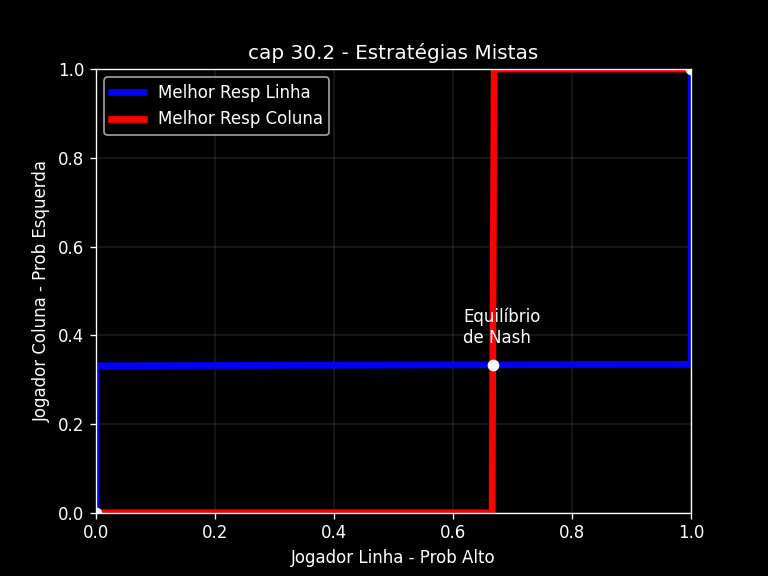
\includegraphics[scale=0.55]{cap30_2-estrategias_mistas.png}
	\end{figure}
	
\end{frame}

\begin{frame}
	\frametitle{Jogos de Coordenação}

	De posse das curvas de melhor resposta, vamos começar a investigar algumas classes de jogos. 
	\\~\\
	A primeira que veremos são os \textbf{jogos de coordenação}: jogos onde os ganhos serão maiores se os jogadores decidirem coordenar suas estratégias. 
	\\~\\
	A questão é criar os mecanismos que criem os incentivos à essa coordenação.

\end{frame}

\begin{lrbox}{\mybox} %\begin{center}\usebox{\mybox}\end{center}
	\def\sgtextcolor{black}% Trocar pra preto na versão white
	\def\sglinecolor{black}% Trocar pra preto na versão white
	\begin{game}{2}{2}[Rapaz][Moça]
		& $Acao$     & $Arte$ \\
		$Acao$   & $2,1$      & $0,0$ \\
		$Arte$   & $0,0$       & $1,2$
	\end{game}
\end{lrbox}

\begin{frame}
	\frametitle{Jogos de Coordenação - Batalha dos Sexos}

	Imagine que temos dois jovens enamorados. Ambos marcaram que iriam se encontrar no cinema, mas estão sem celular e não sabem qual filme o outro verá. O rapaz prefere o filme de ação enquanto a moça prefere o filme de arte. Ambos preferem assistir a algum filme juntos do que não se encontrarem. 
	\\~\\
	Podemos traduzir essa estrutura em uma matriz de ganhos

	\begin{center}\usebox{\mybox}\end{center}

\end{frame}

\begin{frame}
	\frametitle{Jogos de Coordenação - Batalha dos Sexos}

	Já sabemos que essa matriz produz as curvas de melhor resposta vistas na seção passada. Então esse jogo tem 3 equilíbrios. 
	\\~\\
	Nos dois equilíbrios de estratégia pura, teremos as opções: Ambos arriscam se encontrar no filme de Ação, Ambos arriscam se encontrar no filme de Artes. 
	\\~\\
	No equilíbrio de estratégia mista, cada um arriscaria no seu filme preferido com $2/3$ de probabilidade.
	\\~\\
	Se supormos que o rapaz tenha o histórico de ceder as decisões para a moça, podemos definir que esse jogo teria um equilíbrio "mais natural"\ que os outros. O termo comumente usado para essa diferenciação dos equilíbrios é \textbf{ponto focal} do jogo.

\end{frame}

\begin{lrbox}{\mybox} %\begin{center}\usebox{\mybox}\end{center}
	\def\sgtextcolor{black}% Trocar pra preto na versão white
	\def\sglinecolor{black}% Trocar pra preto na versão white
	\begin{game}{2}{2}[Jogador A][Jogador B]
		& $Confessa$      & $Nega$ \\
		$Confessa$  & $-3,-3$         & $0,-6$ \\
		$Nega$      & $-6,0$          & $-1,-1$
	\end{game}
\end{lrbox}

\begin{frame}
	\frametitle{Jogos de Coordenação - Dilema do Prisioneiro}

	Sabemos que a estratégia dominante é confessar. Mas também sabemos que a estratégia eficiente no sentido de Pareto é negar.

	\begin{center}\usebox{\mybox}\end{center}

	Quando modelamos as funções de melhor resposta. Como já sabemos, a única estratégia de equilíbrio é no ponto "confessa-confessa".

\end{frame}

\begin{frame}
	\frametitle{Jogos de Coordenação - Dilema do Prisioneiro}

	\begin{figure}[H]
		\centering
		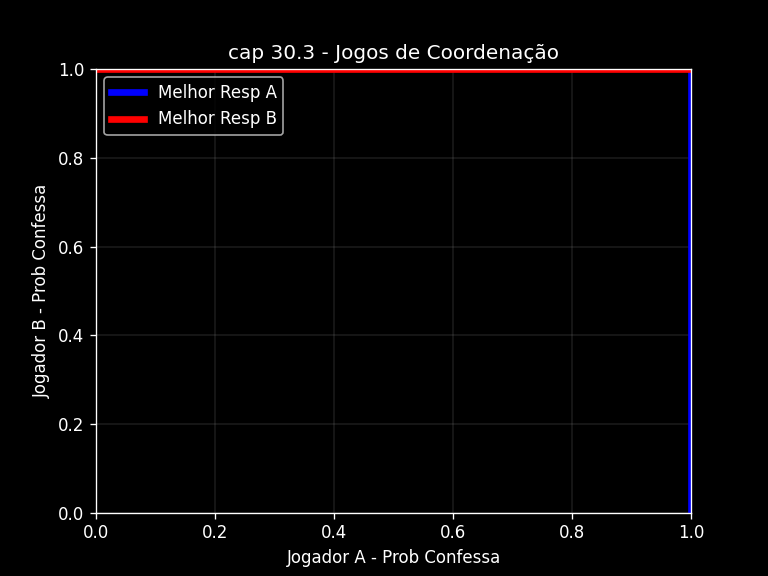
\includegraphics[scale=0.55]{cap30_3-jogos_coordenacao_1.png}
	\end{figure}
		

\end{frame}

\begin{lrbox}{\mybox} %\begin{center}\usebox{\mybox}\end{center}
	\def\sgtextcolor{black}% Trocar pra preto na versão white
	\def\sglinecolor{black}% Trocar pra preto na versão white
	\begin{game}{2}{2}[EUA][URSS]
		& $Abstem$      & $Constroi$ \\
			$Abstem$    & $4,4$         & $1,3$ \\
			$Constroi$  & $3,1$         & $2,2$
		\end{game}
\end{lrbox}

\begin{frame}
	\frametitle{Jogos de Coordenação - Jogos de Garantia}

	Pensemos na corrida amarmentista de meados do século XX. Todo mundo sabe que o melhor era optar por não construir mais mísseis nucleares, o problema, é que você pode ser surpreendido por uma trapaça do outro lado. Podemos resumir esse cenário na tabela abaixo

	\begin{center}\usebox{\mybox}\end{center}

	Como será o gráfico das curva de melhor resposta?

\end{frame}

\begin{frame}
	\frametitle{Jogos de Coordenação - Jogos de Garantia}

	\begin{figure}[H]
		\centering
		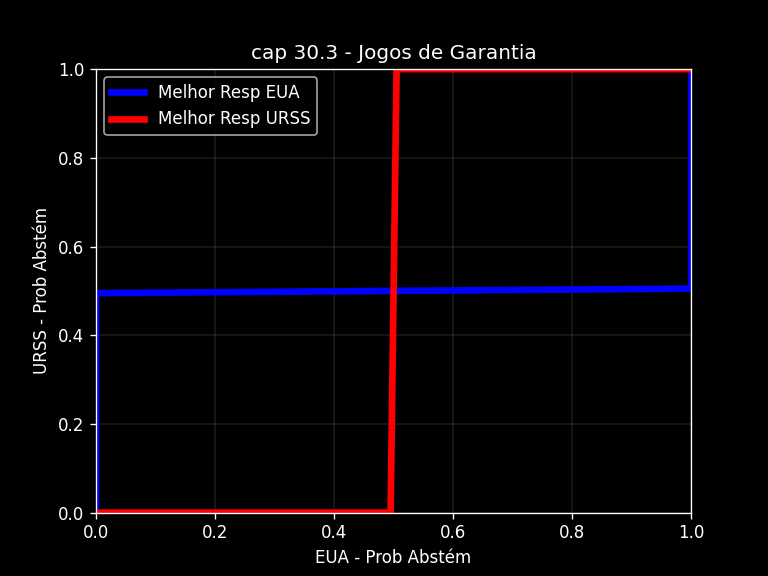
\includegraphics[scale=0.55]{cap30_3-jogos_coordenacao_2.png}
	\end{figure}

\end{frame}

\begin{frame}
	\frametitle{Jogos de Coordenação - Jogos de Garantia}

	Como esse jogo é simultâneo, não temos uma estratégia mista. 
	\\~\\
	Só temos os pontos de equilíbrio nos extremos. 
	\\~\\
	Se um dos participantes conseguir convencer o outro que se abstém, ele "empurrará"\ o outro jogador para o ponto de equilíbrio da abstenção. 
	\\~\\
	A questão toda era como sinalizar de maneira eficiente para o outro jogador e ainda não parecer que está desistindo da corrida.

\end{frame}

\begin{lrbox}{\mybox} %\begin{center}\usebox{\mybox}\end{center}
	\def\sgtextcolor{black}% Trocar pra preto na versão white
	\def\sglinecolor{black}% Trocar pra preto na versão white
	\begin{game}{2}{2}[Linha][Coluna]
		& $Desvia$    & $Mantem$ \\
		$Desvia$   & $0,0$       & $-1,1$ \\
		$Mantem$   & $1,-1$      & $-2,-2$
	\end{game}
\end{lrbox}

\begin{frame}
	\frametitle{Jogos de Coordenação - Roleta Russa}

	Uma prática chamada "roleta russa"\ consiste em dois veículos um de frente para o outro à uma distância considerável. 
	\\~\\
	Os veículos aceleravam em direção ao outro. A ideia é que o motorista mais corajoso não desviaria a trajetória. A matriz de ganhos pode ser definida como

	\begin{center}\usebox{\mybox}\end{center}

	Diferente dos outros jogos, aqui os equilíbrios são nas opções contrárias. Os equilíbrios de Nash de estratégia pura estão nas opções onde eles seguem ações diferentes.
	
\end{frame}

\begin{frame}
	\frametitle{Jogos de Coordenação - Roleta Russa}

	\begin{figure}[H]
		\centering
		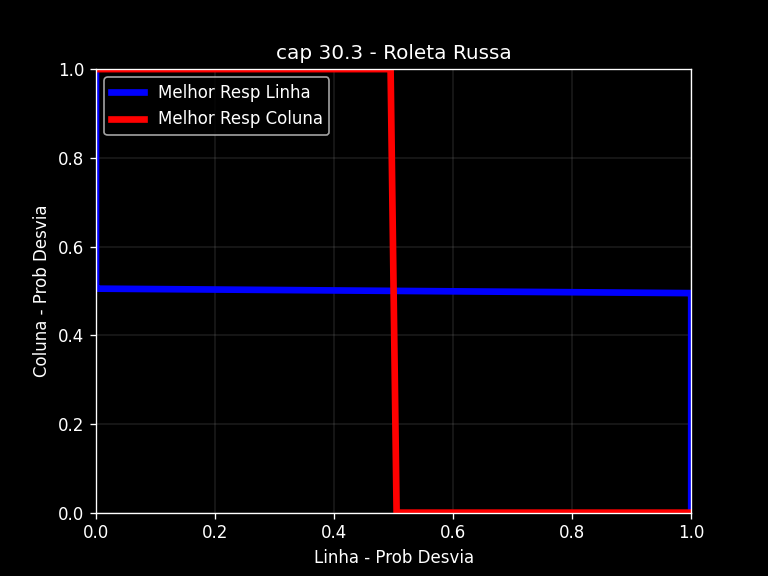
\includegraphics[scale=0.55]{cap30_3-jogos_coordenacao_3.png}
	\end{figure}
		
\end{frame}

\begin{frame}
	\frametitle{Jogos de Coordenação - Roleta Russa}

	Como encontrar um resultado? 
	\\~\\
	A melhor maneira de encontrar um desfecho é pela sinalização de compromisso. 
	\\~\\
	Se um dos competidores arrancasse fora o volante, ele jogaria para o outro motorista toda a responsabilidade pelo resultado. 
	\\~\\
	Nesse caso, a matriz seria atualizada e seria melhor para o outro motorista sair derrotado do que bater o carro.

\end{frame}

\begin{frame}
	\frametitle{Jogos de Coordenação - Como Coordenar?}

	Podemos modificar os resultados pela adoção de movimentos sequenciados, repetição ou contratação.
	\\~\\
	Quando modificamos os jogos da segurança, batalha dos sexos e roleta russa, para jogos sequenciados. Um jogado faz o primeiro movimento, o outro terá que maximizar apenas a partir do movimento feito. 
	\\~\\
	No caso da roleta russa, isso daria a vitória a um delas. Nos outros jogos, isso levaria ao ponto eficiente de Pareto.
	\\~\\
	No caso do dilema do prisioneiro, o melhor a fazer seria modificar o jogo para repetição (que permitiria a retalhação por mal comportamento) ou a contratação (que modificaria o resultado da confissão).

\end{frame}

\begin{lrbox}{\mybox} %\begin{center}\usebox{\mybox}\end{center}
	\def\sgtextcolor{black}% Trocar pra preto na versão white
	\def\sglinecolor{black}% Trocar pra preto na versão white
	\begin{game}{2}{2}[Artilheiro][Goleiro]
							& $Esquerda$    & $Direita$ \\
	$Esquerda$   & $50,-50$      & $80,-80$ \\
	$Direita$    & $90,-90$      & $20,-20$
	\end{game}
\end{lrbox}

\begin{frame}
	\frametitle{Jogos de Competição}

	Os esportes são um bom exemplo desse tipo de arranjo para um \textbf{jogo de soma zero}.

	\begin{center}\usebox{\mybox}\end{center}

	Os valores são variáveis porque simbolizam as probabilidades de gol.
	\\~\\
	Esse é um exemplo de uma \textbf{estratégia mista}.
	\\~\\
	Como esse jogo é competitivo, não teremos opções de equilíbrio em estratégia pura cooperativos.	Infelizmente, não temos tempo de desenvolver os cálculos das funções de melhor resposta, mas você pode conferir no material e no livro.

\end{frame}

\begin{frame}
	\frametitle{Jogos de Competição}

	\begin{figure}[H]
		\centering
		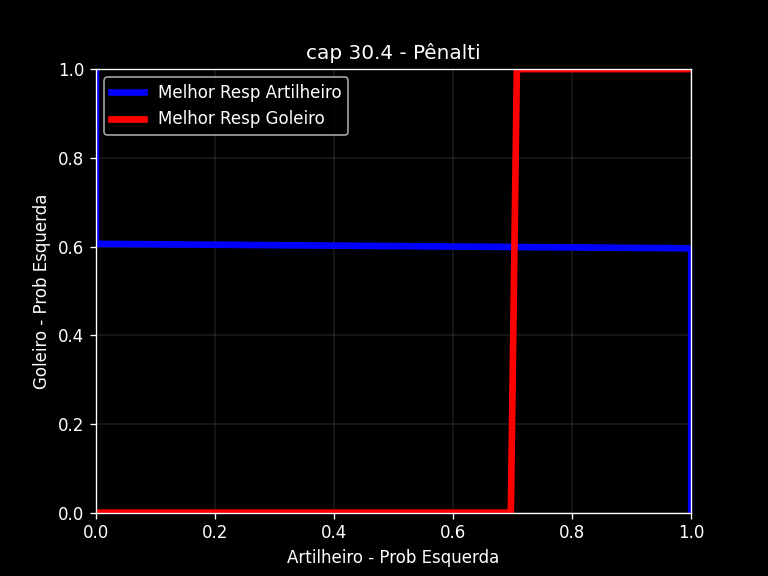
\includegraphics[scale=0.55]{cap30_4-jogos_competitivos.png}
	\end{figure}

\end{frame}

\begin{lrbox}{\mybox} %\begin{center}\usebox{\mybox}\end{center}
	\def\sgtextcolor{black}% Trocar pra preto na versão white
	\def\sglinecolor{black}% Trocar pra preto na versão white
	\begin{game}{2}{2}[Animal linha][Animal coluna]
		& $Lutar$    & $Dividir$ \\
		$Lutar$    & $-2,-2$    & $4,0$ \\
		$Dividir$  & $0,4$      & $2,2$
	\end{game}
\end{lrbox}

\begin{frame}
	\frametitle{Jogos de Coexistência}

	Imagine que exista uma espécie de cachorro selvagem. Se dois animais encontram um pedaço de comida, eles têm de decidir entre brigar ou dividir. O nome dessa interação é \textbf{jogo de pombos e falcões}. A matriz dos ganhos está abaixo

	\begin{center}\usebox{\mybox}\end{center}

	Veja que nenhum dos quadrantes iguais é estável. Se ambos lutarem, é melhor abrir mão do que sair ferido. Se ambos dividirem, é melhor atacar para ficar com tudo.

\end{frame}

\begin{frame}
	\frametitle{Jogos de Coexistência}

	Ao invés de pensarmos em apenas dois animais com escolhas variáveis ao longo do tempo, podemos supor que temos um grupo de animais que se comportarão de maneira diferente. 
	\\~\\
	Nesse modelo, as probabilidades fazem jus a quantidade esperada de cada grupo de animais em cada interação.
	\\~\\
	A probabilidade de algum animal lutar será dada por $p$, assim, a chance de um lutador encontrar outro é de $p$ e de encontrar um disposto a dividir será igual a $1 - p$.

\end{frame}

\begin{frame}
	\frametitle{Jogos de Coexistência}

	O ganho esperado para os lutadores será de

	$$H = -2p + 4(1-p)$$

	Enquanto o ganhos dos que dividirão

	$$D = 2(1-p)$$

	Supondo que as características sejam transferidas, o grupo com o maior retorno terá a maior chance de ser encontrado. Se $H > D$, então veremos a população dos brigões aumentar. Caso $D > H$, então, a população de cooperadores aumentará.

\end{frame}

\begin{frame}
	\frametitle{Jogos de Coexistência}

	O equilíbrio entre essas populações será dado pela igualdade

	$$H = -2p + 4(1-p) = 2(1-p) = D$$
	$$2(1-p) = 2p$$
	$$2 - 2p = 2p$$
	$$p = 1/2$$

	Agora vamos ver como se comportam as curvas de melhor resposta.

\end{frame}

\begin{frame}
	\frametitle{Jogos de Coexistência}

	Por causa da estabilidade desse arranjo, os pesquisadores o classificam como uma \textbf{estratégia evolucionariamente estável}. 
	\\~\\
	É pura teoria dos jogos e vem diretamente dos estudos das dinâmicas entre interações animais.

\end{frame}

\begin{frame}
	\frametitle{Jogos de Coexistência}

	\begin{figure}[H]
		\centering
		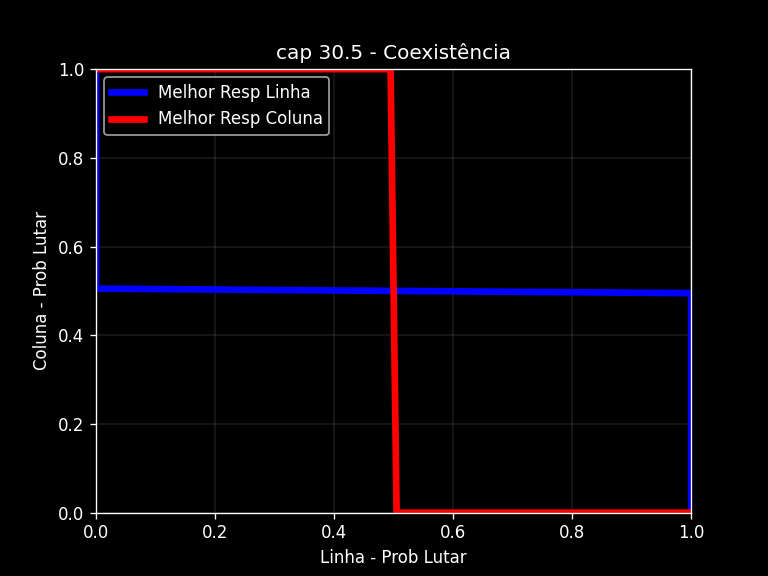
\includegraphics[scale=0.55]{cap30_5-coexistencia_1.png}
	\end{figure}
		
\end{frame}

\begin{frame}
	\frametitle{Jogos de Coexistência}

	Aqui vemos 3 condições de equilíbrio. Mas nosso equilíbrio não foi alcançado no ponto $1/2$? A resposta é sim. 
	\\~\\
	Perceba que os pontos de estratégia dominante são os pontos onde há o incentivo de se jogar o oposto do adversário\footnote{Igual o caso da roleta russa}. 
	\\~\\
	Mas esse jogo não lida com apenas 2 agentes e sim com uma população homogênea com duas opções de comportamento. 
	\\~\\
	O único ponto onde as estratégias convergem é o ponto $1/2$.
	\\~\\
	Assim como está no livro, eu coloquei os resultados para cada estratégia a medida que o número de lutadores aumenta de $0$ até $100\%$.

\end{frame}

\begin{frame}
	\frametitle{Jogos de Coexistência}

	\begin{figure}[H]
		\centering
		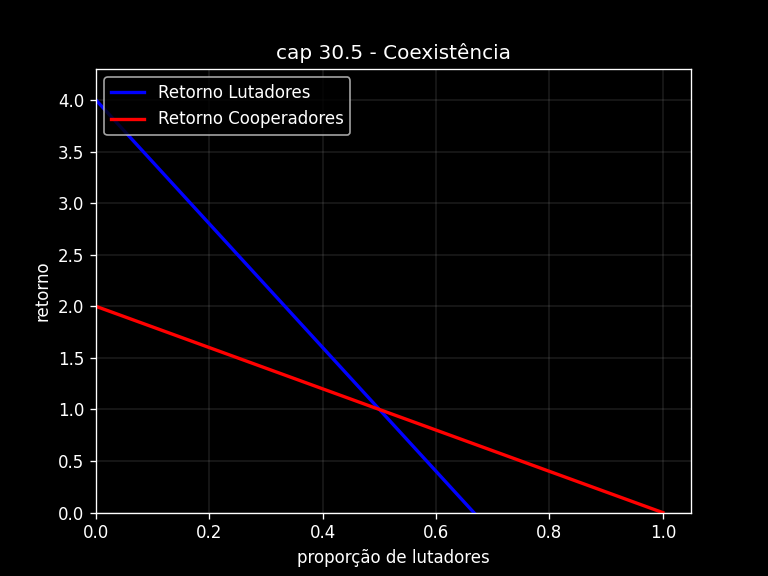
\includegraphics[scale=0.55]{cap30_5-coexistencia_2.png}
	\end{figure}

\end{frame}

\begin{frame}
	\frametitle{Jogos de Compromisso}

	Os jogos que vimos até agora são do jogos \textbf{com movimentos simultâneos}. Os jogadores não sabem o que o outro fará, e precisam maximizar de acordo com a suposição do comportamento do adversário.
	\\~\\
	Aqui vamos ver os jogos com \textbf{movimento sequenciais}. Um conceito importante nesses jogos é o \textbf{compromisso}. 
	\\~\\
	Quando um participante se compromete a agir de terminada maneira ele precisa garantir: 1) que ele não terá outro caminho a seguir além do firmado anteriormente; 2) que a sinalização do compromisso chegue ao outro jogador e seja entendida por ele.

\end{frame}

\begin{frame}
	\frametitle{Jogos de Compromisso - O Sapo e o Escorpião}

	Vocês já devem conhecer essa história.

	\Tree[.\textit{Sapo}
				[.Carrega 
					[.Escorpião 
						[.Ferroada $(-10,5)$ ]
						[.\textit{Não Ferroada} $(5,3)$ ]]]
				[.\textit{Não Carrega} $(0,0)$ ]]
	\\
	\ 
	\\
	Mesmo que a moral da história seja nós ensinar que existem pessoas que preferem fazer o mal. Nós somos economistas, e, como de costume, vamos estragar mais essa história.


\end{frame}

\begin{frame}
	\frametitle{Jogos de Compromisso - O Sapo e o Escorpião}

	Sob a ótica da teoria dos jogos, o escorpião apenas maximizou sua utilidade dada as opções disponíveis. Como o sapo escolheu antes, só restou ao escorpião entre ter $5$ de retorno com a ferroada ou $3$ com o passeio.
	\\~\\
	Se o sapo tivesse a oportunidade de ver essa aula, ele se certificaria em reduzir o resultado do escorpião na opção da ferroada.
	\\~\\
	As opções são muitas: Falar como é bom estar vivo; Ameaçar toda a família do escorpião; Amarrar a calda dele antes de sair. Todas essas arbodagens atuam na mudança da matriz de ganhos do escorpião.
	\\~\\
	Na versão desse conto dos economistas, o sapo chegaria do outro lado e a moral da história seria como é bom fazer o bem independente a quem.

\end{frame}

\begin{frame}
	\frametitle{Jogos de Compromisso - O Sequestrador Cordial}

	Imagine que um CEO de uma empresa é sequestrado. No regimento interno da empresa está a cláusula de não pagamento de resgate em caso de sequestro dos seus funcionários (mesmo os da cúpula). O que os sequestradores farão? Uma possibilidade de arranjo é esse abaixo

	\Tree[.\textit{Sequestradores}
					[.Libera 
						[.Refém 
							[.Identifica $(-5,5)$ ]
							[.\textit{Não Identifica} $(5,3)$ ]]]
					[.\textit{Mata} $(-3,-10)$ ]]

\end{frame}

\begin{frame}
	\frametitle{Jogos de Compromisso - O Sequestrador Cordial}

	O resultado desse jogo é inteiramente dependente da capacidade do refém de sinalizar para os sequestradores que cumprirá seu lado do trato em não identificar. 
	\\~\\
	O que vocês proporiam para sair dessa situação?
	\\~\\
	Uma saída (genial) para esse impasse é a proposta pelo pesquisador Thomas Schelling.

\end{frame}

\begin{frame}
	\frametitle{Jogos de Compromisso - Poupanças e Seguridade Social}

	Agora vamos aplicar nossos conceitos ao modelos de seguridade social. Podemos modelar esse jogo como uma relação entre gerações do seguinte modo

	\Tree[.\textit{Velhos}
				[.Poupam 
					[.Jovens 
						[.Sustentam $(2,-1)$ ]
						[.Poupam $(1,0)$ ]]]
				[.Esbajam
					[.Jovens 
						[.Sustentam $(3,-1)$ ]
						[.Poupam $(-2,-2)$ ]]]]

\end{frame}

\begin{frame}
	\frametitle{Jogos de Compromisso - Poupanças e Seguridade Social}

	Conseguimos ver que a melhore estratégia para os velhos é usar o poder da preferência e escolher esbanjar. 
	\\~\\
	Os jovens serão obrigados a optar por sustentá-los. 
	\\~\\
	Mas não é atoa que a maioria dos países possui algum programa em que cada geração acaba contribuindo para o montante da sua aposentadoria.

\end{frame}

\begin{frame}
	\frametitle{Jogos de Compromisso}

	No material e no livro existem mais dois jogos que não teremos tempo de arbodar aqui: Onde a força é fraqueza e Extorção.
	\\~\\
	No primeiro, mesmo que uma das partes tenha poder de subjulgar a outra, a parte mais fraca fica na vantagem porque ela simplesmente decide não agir (e não pode ser obrigada a isso).
	\\~\\
	Na extorção temos um caso onde a obra está terminando e o pedreiro tira vantagem disso pra cobrar preços abusivos. A saída dessa cilada é ter feito um contrato inicialmente ou ameaçar queimar o nome do pedreiro na praça.

\end{frame}

\begin{frame}
	\frametitle{Negociação}

	Nessa última parte do capítulo, pensemos em um problema simples: a divisão de um dólar entre duas pessoas. Como faríamos de modo a satisfazer a vontade de ambas? O foco está em construir uma solução que permita a negociação.
	\\~\\
	Existem um modelo chamado \textbf{modelo de negociação de Nash}, usa uma abordagem a partir de proposições a respeito do comportamento dos indivíduos. Mas ele é demasiadamente complexo para o escopo de curso.
	\\~\\
	Uma outra abordagem é o \textbf{modelo de negociação de Rubinstein}. Esse modelo o livro explica um pouco mais, contudo, sem entender o básico de matemática financeira fica difícil entender. Deixemos pra outro dia.

\end{frame}


%%%%%%%%%%%%%%%%%%%%%%%%%%%%%%%%%%%%%%%%%%%
\section[E.Comport.]{Economia Comportamental}
%%%%%%%%%%%%%%%%%%%%%%%%%%%%%%%%%%%%%%%%%%%
\begin{frame}
	\huge Economia Comportamental \normalsize
	\\~\\
	\begin{itemize}
		\item Efeitos do Contexto
		\item Incerteza
		\item Tempo
		\item Interação e Normas Sociais
		\item O que fazer agora?
	\end{itemize}
\end{frame}


\begin{frame}
	\frametitle{Efeitos do Contexto}

	Uma das novidades que esse campo trouxe, foi o papel que o \textbf{contexto} e o \textbf{modo} as escolhas são apresentadas têm no resultado do processo de decisão. 
	\\~\\
	A percepção do mesmo produto em lojas diferentes muda o preço de reserva das pessoas. 
	\\~\\
	Produtos com valores quebrados (os benditos $0,99$ de quase todos os preços que vemos) costumam performar diferente dos produtos de preços cheios. 
	\\~\\
	A lista de \textbf{efeitos de contexto} é bem grande. Vamos ver agora alguns dos vieses que já conseguimos observar em alguns experimentos.

\end{frame}

\begin{frame}
	\frametitle{Efeitos do Contexto - O Dilema da Doença}

	Imagine que existe uma doença ameaçando uma população de 600 pessoas. Você pode escolher entre dois tratamentos, A e B, com as seguintes características:
	\\~\\
	\textbf{Tratamento A:} 200 pessoas salvas, de certeza.\\
	\textbf{Tratamento B:} 1/3 de probabilidade de salvar as 600 pessoas e 2/3 de que todos morram.
	\\~\\
	Se fossem descobertos outros dois tratamentos.
	\\~\\
	\textbf{Tratamento C:} 400 pessoas vão morrer, de certeza.\\
	\textbf{Tratamento D:} 2/3 de probabilidade das 600 pessoas morrerem e 1/3 de chance de salvar todos.

\end{frame}

\begin{frame}
	\frametitle{Efeitos do Contexto - O Dilema da Doença}

	No \textbf{contexto positivo}, as pessoas optaram na maioria pela opção A.
	\\~\\
	No \textbf{contexto negativo}, D foi escolhido com maior frequência. O estranho é que A, B, C e D são todas equivalente!
	\\~\\
	Esse exemplo pode ser aplicado a uma gama de outras situações, como gestão de portfólio. Será que as pessoas pensam com a mesma tranquilidade em momentos de alta e de baixa de ações?

\end{frame}

\begin{frame}
	\frametitle{Efeitos do Contexto - Efeito Ancoragem}

	O \textbf{efeito ancoragem} é definido como o efeito que algumas informações complemente não relacionadas ao objeto de decisão pode exercer no processo mental de escolha.
	\\~\\
	Um exemplo desse efeito foi a escolha de qual investimento os empregador escolheriam no seu plano de aposentadoria dos seus empregados.
	\\~\\
	Quando os empregadores faziam a pergunta de adesão com uma opção de investimento previamente marcada, a maioria das pessoas optava por seguir a recomendação. 
	\\~\\
	Quando foi feito o mesmo experimento em outra empresa, mas sem a previa marcação, o perfil de seleção mudou.

\end{frame}

\begin{frame}
	\frametitle{Efeitos do Contexto - Balizamento}

	Quando foi proposto que um time de estudantes escolhesse, entre seis opções por dia, o seu menu de lanches para as próximas três semanas. A maioria optou por um tipo para cada dia da semana. 
	\\~\\
	Mas quando a escolha era feita na hora, mesmo tendo as seis opções, a maioria das pessoas escolheu repetir alguma refeição do dia anterior.
	\\~\\
	Nós agimos diferentemente quando planejamos com antecedência e quando tempos que decidir na hora.

\end{frame}

\begin{frame}
	\frametitle{Efeitos do Contexto - Excesso de Opções}

	Nós vimos que uma das soluções de equilíbrio de competição monopolística é o excesso de opções. Ao buscar a diferenciação dos seus produtos, os concorrentes podem impor uma sobrecarga de opções aos seus consumidores.
	\\~\\
	Fora montado em um supermercado dois expositores de geleia. Um com 26 opções e outro com apenas 6. 
	\\~\\
	As pessoas paravam mais no expositor com mais opções, entretanto, a maioria das vendas foi realizada no expositor com menos produtos. 
	\\~\\
	Em 2001, Shlomo Benartzi e Richard Thaler mostraram que essa lógica também pode ser aplicada ao mercado de ativos.

\end{frame}

\begin{frame}
	\frametitle{Incerteza - Lei dos Pequenos Números}

	A ideia aqui é que as pessoas tendem a se influenciar muito a partir de pequenas amostras. Ainda mais, se elas mesmas que fizeram a observação.
	\\~\\
	Imagine dois hospitais. Um com 100 leitos, outro com 15 leitos. Por dia, nascem aproximadamente 11 bebês no hospital maior e 5 no menor. Se estivermos interessados em saber todos os dias em que tivermos a maioria de nascidos homens. 
	\\~\\
	Qual hospital teria o maior número de registros desses dias em um ano?

\end{frame}

\begin{frame}
	\frametitle{Incerteza - Integração de Ativos e Aversão à Perda}

	É comum supor que as pessoas se importam com o total de riqueza que receberiam através dos diversos estados possíveis. Esse pressuposto é chamado de \textbf{hipótese da integração de ativos}.
	\\~\\
	Imagine que sua renda é 10.000 e seja proposta uma aposta de cara e coroa. Se der cara, você ganha R\$14,00, se der coroa, você paga R\$ 10,00. O retorno esperado é de R\$ 2,00, ou seja, essa aposta vale a pena. 
	\\~\\
	Mas, na prática, muita gente não topa.

\end{frame}

\begin{frame}
	\frametitle{Tempo - Desconto}

	Quando trabalhamos a percepção do valor ao longo do tempo, geralmente precisamos supor uma forma funcional de desconto. A forma do \textbf{desconto exponencial} é dada por $\delta^t u(c)$ onde $\delta < 1$. 
	\\~\\
	Outra forma é a do \textbf{desconto hiperbólico}, que veio em um estudo sobre precificações de valores futuros por meio de leilão, afirma que a taxa de desconto seria $\frac{u(c)}{(1+kt)}$.
	\\~\\
	O problema dessa diferença é que, enquanto o desconto exponencial é consistente ao longo do tempo, o hiperbólico atribui diferentes pesos dependendo do período. Isso pode implicar em planejar de uma maneira e agir de outra.

\end{frame}

\begin{frame}
	\frametitle{Tempo - Autocontrole}

	Não é raro encontrar situações onde acabamos nos encontrando em situações que prometemos não fazer. O fator importante a ser levado em conta é justamente a nossa capacidade de modelar nosso próprio \textbf{autocontrole}, ou melhor, a falta dele.
	\\~\\
	Uma maneira de reforçar essa capacidade é, como vimos nos jogos sequenciados, o comprometimento.
	\\~\\
	O importante aqui é saber que os modelos mais reais precisam levar em consideração a capacidade das pessoas não seguirem exatamente os planos que fizeram.

\end{frame}

\begin{frame}
	\frametitle{Interação e Normas Sociais - Jogo do Ultimato}

	Existe um campo chamado \textbf{teoria comportamental do jogo} que analisa como as pessoas agem, na vida real, em situações diversas.
	\\~\\
	Já vimos que, do ponto de vista teórico, não existe nenhum motivo para uma pessoa negar a divisão de 0,90 e 0,10. Visto que é melhor 0,10 do que nada! Mas não é assim que observamos  na prática. 
	\\~\\
	Quando a divisão proposta é muito desigual, as pessoas preferem ficar com 0 do que com míseros trocados.

\end{frame}

\begin{frame}
	\frametitle{Interação e Normas Sociais - Equidade}

	Parece que temos alguma tendência à divisões iguais. Mesmo que essas \textbf{normas de equidade} não causem um resultado interessante para nós mesmos.
	\\~\\
	Quando colocamos uma terceira parte num \textbf{jogo punitivo} - igual ao jogo do ultimato só que generalizado - com poder de subtrair parte do lucro do proponente, acabamos vendo um padrão. 
	\\~\\
	Quando a divisão é muito desigual, esses terceiros acabam optando por punir o proponente ganancioso.

\end{frame}

\begin{frame}
	\frametitle{O que fazer agora?}

	Como todas essas situações podem ser interpretadas à luz da teoria que já estamos acostumados? A chave é aceitar que as preferências não são construtos sólidos e perenes do nosso ser, mas sim, "descobertas"\ que fazemos ao longo dos processos de decisão.
	\\~\\
	Se uma pessoa pega um produto na prateleira, devolve, depois volta e pega o mesmo produto novamente, ela prefere ou não esse bem? 
	\\~\\
	À luz dessas descobertas, podemos dizer que a pessoa está no limiar entre a escolha ou não do produto. É como se ela mesma ainda não soubesse o que quer, ou seja, é como se estivesse "descobrindo"\ sua suas próprias preferências.

\end{frame}

\begin{frame}
	\frametitle{O que fazer agora?}

	Precisamos jogar a teoria da escolha fora? 	Nós perdemos nosso precioso tempo estudando esse modelo para nada? 
	\\~\\
	Mesmo que as preferências não sejam inerentes e imutáveis, uma vez que testamos e redescobrimos as preferências por meio de escolhas, podemos ver que, mesmo ainda não compreendendo o processo, essas preferências se tornam balizadoras das próximas escolhas. 
	\\~\\
	Nós tendemos a repetir padrões de escolhas com razoável confiança preditiva. O motivo de preferir A em relação B, pode ser um mistério, mas nosso modelo de teoria da escolha não se preocupa com isso.

\end{frame}

%%%%%%%%%%%%%%%%%%%%%%%%%%%%%%%%%%%%%%%%%%%
\section[Trocas]{Trocas}
%%%%%%%%%%%%%%%%%%%%%%%%%%%%%%%%%%%%%%%%%%%
\begin{frame}
	\huge Trocas \normalsize
	\\~\\
	\begin{multicols*}{2}		
	\begin{itemize}
		\item A Caixa de Edgeworth
		\item As Trocas
		\item Alocações Pareto Eficientes
		\item Trocas de Mercado
		\item Álgebra do Equilíbrio
		\item Lei de Walras
		\item Preços Relativos
		\item Existência de Equilíbrio
		\item Equilíbrio e Eficiência
		\item Álgebra da Eficiência
		\item Eficiência e Equilíbrio
		\item 1º Teorema do Bem-Estar
		\item 2º Teorema do Bem-Estar
	\end{itemize}
\end{multicols*}
\end{frame}

\begin{frame}
	\frametitle{Equilíbrio Geral}

	Todos os equilíbrios que estudamos até agora se basearam apenas nas relações de preço e quantidade de determinado bem e nas equivalências entre as forças de Oferta e Demanda. 
	\\~\\
	O equilíbrio dentro de um mercado apenas é chamado de \textbf{equilíbrio parcial}.
	\\~\\
	Começaremos a partir de agora o estudo de equilíbrio \textit{entre} diferentes mercados. O nome dessa agenda de pesquisa é \textbf{equilíbrio geral}.

\end{frame}

\begin{frame}
	\frametitle{Equilíbrio Geral}

	Como lidaremos com múltiplos mercados ao mesmo tempo, a análise se torna bastante complexa. Para tanto, vamos nos valer de algumas simplificações para facilitar a nossa vida:
	\\~\\
	\begin{itemize}
		\item Mercados são competitivos, ou seja, não existe poder de mercado.
		\item Número limitado de bens e consumidores\footnote{Mas saibam que as soluções que acharmos podem ser expandidas para $n$ bens e indivíduos.}.
		\item Nesse primeiro momento, usaremos o sistema de trocas puras sem produção.
	\end{itemize}

\end{frame}

\begin{frame}
	\frametitle{A Caixa de Edgeworth}

	Um economista inglês do século XIX chamado Francis Ysidro Edgeworth criou uma ferramenta analítica que usaremos para analisar os casos de trocas entre dois indivíduos. A famosa \textbf{caixa de Edgeworth}.
	\\~\\
	Suporemos a existência de duas pessoas, A e B, e dois bens, 1 e 2. A cesta do consumidor A será denotada por $X_A = (x_A^1, x_A^2)$, similarmente, a cesta de B será dada por $X_B = (x_B^1, x_B^2)$. 
	\\~\\
	Um par de cestas será chamado de \textbf{alocação}. A \textbf{dotação inicial} é uma alocação que indica a condição inicial de cada agente e é denotado por $W_A = (w_A^1,w_A^2)$ e $W_B = (w_B^1,w_B^2)$.

\end{frame}

\begin{frame}
	\frametitle{A Caixa de Edgeworth}

	Uma alocação será chamada de \textbf{factível} se a quantidade total for igual a 

	$$x_A^1 + x_B^1 = w_A^1 + w_B^1$$
	$$x_A^2 + x_A^2 = w_A^2 + w_A^2$$
	\\~\\
	Após a etapa de trocas, chegaremos em outra alocação factível importante, a \textbf{alocação final}.
	\\~\\
	Veremos um exemplo da caixa de Edgeworth. Foram usadas funções de utilidade do tipo cobb-douglas com os coeficientes iguais a $0.5$.

\end{frame}

\begin{frame}
	\frametitle{A Caixa de Edgeworth}

	\begin{figure}[H]
		\centering
		\colorbox{black}{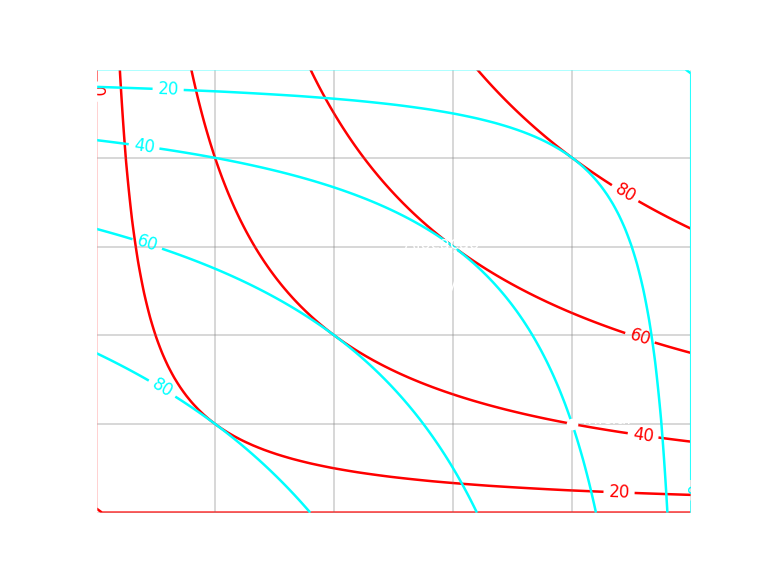
\includegraphics[scale=0.6]{cap32_1-caixa_edgeworth_1.png}}
	\end{figure}

\end{frame}

\begin{frame}
	\frametitle{A Caixa de Edgeworth}

	Uma mudança aqui é que estamos representando as preferências de dois consumidores ao mesmo tempo. As curvas vermelhas são do consumidor A e, consequentemente, as curvas azuis são do consumidor B.
	\\~\\
	Isso significa que cada ponto nesse gráfico possui 4 coordenadas associadas $(w_A^1, w_A^2, w_B^1, w_B^2)$ para a dotação e $(x_A^1, x_A^2, x_B^1, x_B^2)$ para a alocação final. 
	\\~\\
	A simetria que podemos ver nas quantidades se dá pela definição das alocações factíveis, onde para um ganhar, outro tem que ceder.

\end{frame}

\begin{frame}
	\frametitle{A Caixa de Edgeworth}

	\begin{figure}[H]
		\centering
		\colorbox{black}{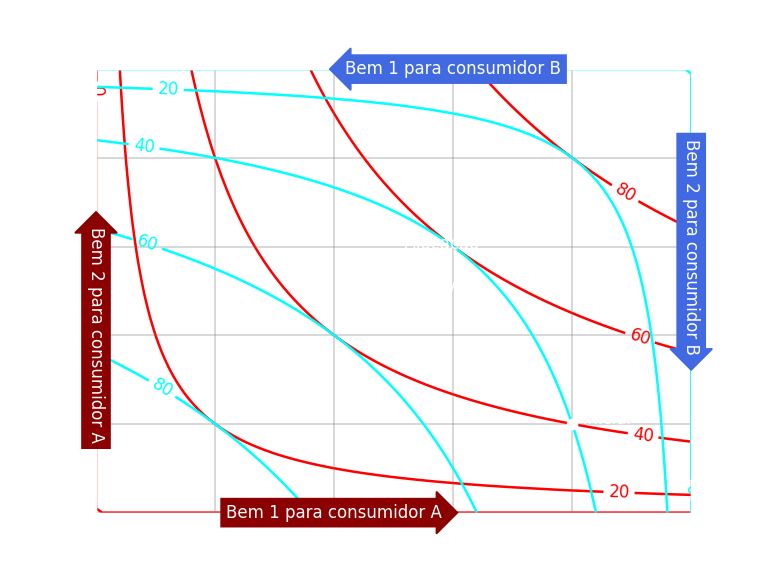
\includegraphics[scale=0.6]{cap32_1-caixa_edgeworth_2.png}}
	\end{figure}

\end{frame}

\begin{frame}
	\frametitle{A Caixa de Edgeworth}

	Esse ferramental analítico nos permite mostrar todas as alocações factíveis, as preferências dos consumidores, a dotação inicial e a alocação final. 
	\\~\\
	Tudo isso de uma vez só. 
	\\~\\
	Não foi sem motivo que esse modelo foi adotado.

\end{frame}

\begin{frame}
	\frametitle{Trocas}

	Para entender o processo de trocas, precisamos analisar o que se passa no momento em que os consumidores se encontram nas suas dotações iniciais.
	\\~\\
	No ponto da dotação inicial da imagem, temos o encontro de duas curvas de indiferenças sendo uma para cada consumidor.
	\\~\\
	O consumidor A gostaria de abrir mão do bem 1 para poder consumir mais do bem 2, já no caso de B, ele quer fazer o oposto, abrir mão de parte da quantidade do bem 2 para consumir mais do bem 1. 
	\\~\\
	Toda a área entre as curvas vermelha e azul representa uma região de melhoria mútua.

\end{frame}

\begin{frame}
	\frametitle{Trocas}

	\begin{figure}[H]
		\centering
		\colorbox{black}{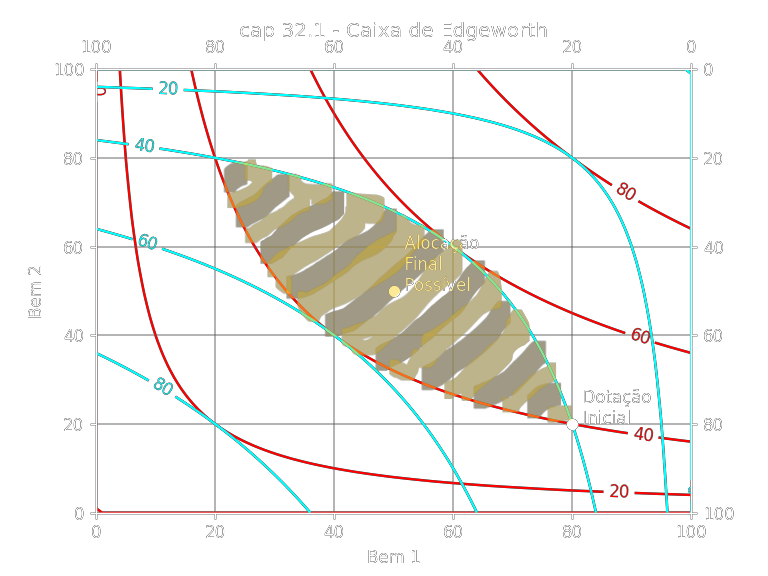
\includegraphics[scale=0.6]{cap32_11-caixa_edgeworth_1.png}}
	\end{figure}

\end{frame}

\begin{frame}
	\frametitle{Trocas}

	As trocas ocorrerão até o ponto em que nenhuma melhoria seria possível sem a piora de um deles. Esse ponto é onde existe tangência das curvas de indiferença.
	\\~\\
	No caso do exemplo, por acaso, o ponto final foi o da divisão igualitária, mas isso não é uma regra.
	\\~\\
	As variações das quantidades em termo das dotações para o consumidor A são dadas por $|x_A^1 - w_A^1|$ para o bem 1 e $|x_A^2 - w_A^2|$ para o bem 2. 
	\\~\\
	Similarmente, $|x_B^1 - w_B^1|$ e $|x_B^2 - w_B^2|$, para o consumidor B.

\end{frame}

\begin{frame}
	\frametitle{Alocações Eficientes no Sentido de Pareto}

	Podemos descrever uma alocação eficiente de Pareto como tendo a seguintes propriedades:
	\\~\\
	\begin{itemize}
		\item Não existe maneira de melhorar a situação de ninguém.
		\item Não existe maneira de melhorar a situação de ninguém, sem que isso implique na piora de outra pessoa.
		\item Todas as trocas que gerariam algum ganho foram feitas.
		\item Não existe opção de troca que seja mutualmente vantajosa.
	\end{itemize}

\end{frame}

\begin{frame}
	\frametitle{Alocações Eficientes no Sentido de Pareto}

	Essas características implicam que os pontos de eficiência sejam pontos em que as curvas de indiferença sejam tangentes entre si. 
	\\~\\
	Pois, se as curvas se cruzam, seria melhor para eles irem para algum ponto em uma curva mais alta, uma vez que, a região no interior do cruzamento de duas curvas é necessariamente, melhor para eles.
	\\~\\
	O conjunto de todos os pontos eficientes no sentido de Pareto, dentro de uma caixa de Edgeworth, é denominado de \textbf{conjunto de Pareto} ou \textbf{curva de contrato}.

\end{frame}

\begin{frame}
	\frametitle{Alocações Eficientes no Sentido de Pareto}


	\begin{figure}[H]
		\centering
		\colorbox{black}{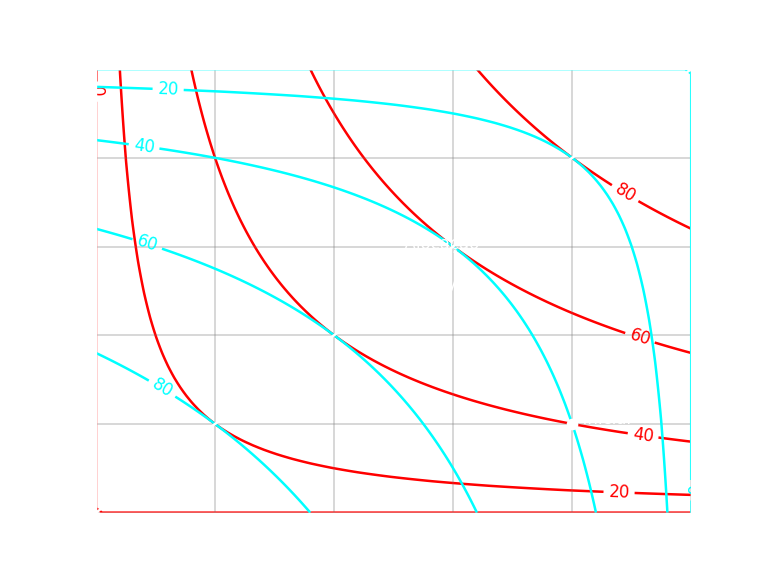
\includegraphics[scale=0.6]{cap32_3-caixa_edgeworth_1.png}}
	\end{figure}		

\end{frame}

\begin{frame}
	\frametitle{Alocações Eficientes no Sentido de Pareto}

	Dada a utilidade qualquer do agente B fixa $\overline{u}$, o problema da maximização da utilidade total do mercado pode ser formalizado como

	\begin{center}
	\LARGE $\stackrel{max}{\text{\small $x_A^1,x_A^2,x_B^1,x_ B^2$}} \ \ \stackrel{u_A(x_A^1,x_A^2)}{\ }$
	\\~\\
	\normalsize de modo que $u_B(x_B^1,x_B^2) = \overline{u}$ \\
	$x_A^1 + x_B^1 = w^1$ \\
	$x_A^2 + x_B^2 = w^2$
	\end{center}
	
\end{frame}

\begin{frame}
	\frametitle{Alocações Eficientes no Sentido de Pareto}

	Primeiramente, podemos escrever nosso problema em forma de uma Lagrangiana 

	$$L(x_A^1,x_A^2,x_B^1,x_B^2) = u_A(x_A^1,x_A^2) - \lambda(u_B(x_B^1,x_B^2) - \overline{u}) $$ 
	$$ - \mu_1(x_A^1 + x_B^1 - w^1) - \mu_2(x_A^2 + x_B^2 - w^2)$$

	A novidade aqui é que temos 3 condições de restrições. Pode até assustar numa primeira vista, mas não é nada impossível.
	\\~\\
	O $\lambda$ é o nosso conhecido multiplicador Lagrangiano, só que aqui, aplicada para a utilidade de B e $\mu$ são os multiplicadores de Lagrange nas restrições dos recursos.

\end{frame}

\begin{frame}
	\frametitle{Alocações Eficientes no Sentido de Pareto}

	As condições de primeira ordem para maximização da nossa Lagrangiana a respeito das 4 variáveis são:

	$$\frac{\partial L}{\partial x_A^1} = \frac{\partial u_A}{\partial x_A^1} - \mu_1 = 0$$
	$$\frac{\partial L}{\partial x_A^2} = \frac{\partial u_A}{\partial x_A^2} - \mu_2 = 0 $$
	$$\frac{\partial L}{\partial x_B^1} = -\lambda \frac{\partial u_B}{\partial x_B^1} - \mu_1 = 0 $$
	$$\frac{\partial L}{\partial x_B^2} = -\lambda \frac{\partial u_B}{\partial x_B^2} - \mu_2 = 0 $$

\end{frame}

\begin{frame}
	\frametitle{Pausa}

	\begin{figure}[H]
		\centering
		\colorbox{white}{
\includegraphics[scale=0.425]{pausa.png}}
	\end{figure}		

\end{frame}


\begin{frame}
	\frametitle{Alocações Eficientes no Sentido de Pareto}

	Lá no capítulo sobre as preferências, nós aprendemos que a taxa marginal de substituição é obtida quando, dada uma função de utilidade $u(x_1,x_2)$, a derivada parcial de $u$ em função de $x_{1}$ divida pela derivada parcial de $u$ em relação à $x_{2}$.
	\\~\\
	Se dividirmos as equações 1 e 2 e depois multiplicarmos por -1, teremos que
	$$TMS_{A} = - \frac{\partial u_A / \partial x_{A}^1 }{\partial u_A / \partial x_{A}^2} = - \frac{\mu_{1} }{ \mu_{2} }$$
	\\~\\
	Se fizermos a mesma coisa para as equações 3 e 4, teremos
	$$TMS_{B} = - \frac{\partial u_B / \partial x_{B}^1 }{\partial u_B / \partial x_{B}^2} = - \frac{\mu_{1} }{ \mu_{2} }$$

\end{frame}

\begin{frame}
	\frametitle{Alocações Eficientes no Sentido de Pareto}

	Também sabemos que, no equilíbrio de um mercado competitivo, as TMS são iguais aos preços, ou seja

	$$ - \frac{\partial u_A / \partial x_{A}^1 }{\partial u_A / \partial x_{A}^2} = - \frac{\partial u_B / \partial x_{B}^1 }{\partial u_B / \partial x_{B}^2} = - \frac{ p_{1} }{ p_{2} } $$
	\\~\\
	Observe que temos uma equivalência entre os multiplicadores de Lagrange $\mu$ e os preços. 
	\\~\\
	Por causa disso, eles até têm nomes especiais, nesse contexto, podem ser chamamos de \textbf{preços-sombra} ou \textbf{preços de eficiência}.

\end{frame}

\begin{frame}
	\frametitle{As Trocas de Mercado}

	Até agora, sabemos que os agentes iniciam nas dotações inicias e terminam em algum ponto na linha de contrato.
	\\~\\
	Como saber "onde"\ exatamente eles vão optar por parar de trocar?
	\\~\\
	Para ter essa resposta, precisaremos adicionar mais informação sobre o comportamento dos nossos consumidores: Esse processo imitará o \textit{resultado} de um mercado competitivo\footnote{O resultado, não o processo.}.

\end{frame}

\begin{frame}
	\frametitle{As Trocas de Mercado}

	Vamos colocar um terceiro indivíduo no processo. Ele agirá com um "leiloeiro"\ para A e B.
	\\~\\
	O leiloeiro vai arbitrar um preço para A e B e eles agirão a partir disso. 
	\\~\\
	Para cada preço arbitrado, os consumidores adaptarão as suas alocações finais aos preços de modo a maximizar suas utilidades. Nesse novo modelo, teremos  um novo dado, a dotação de preços $(p_1,p_2)$.

\end{frame}

\begin{frame}
	\frametitle{As Trocas de Mercado}

	Vamos ver quais informações nós temos disponíveis para trabalhar agora:
	\begin{enumerate}
		\item Uma dotação inicial de bens
		\item Preços associados a cada bem
		\item Preferências de cada consumidor
	\end{enumerate}
	\ 
	\\~\\
	Como vocês passaram por microeconomia I, sabem muito bem que tratamos essas variáveis no capítulo 5 (com a teoria da escolha) e no 9 (com as dotações). Né?!

\end{frame}

\begin{frame}
	\frametitle{As Trocas de Mercado}

	Quando o leiloeiro determina o preço dos bens no mercado, ele automaticamente determina a renda de cada um dos participantes

	$$renda_A = w_A^1 p_1 + w_A^2 p_2$$

	Isso quer dizer que podemos, a partir da dotação inicial, descrever a restrição orçamentária via equação

	$$ x_A^1 p_1 + x_A^2 p_2 = renda_A$$
	$$ x_A^1 p_1 + x_A^2 p_2 = w_A^1 p_1 + w_A^2 p_2$$
	$$ x_A^2 = [(w_A^1 p_1 + w_A^2 p_2) - x_A^1 p_1]/p2$$

	Visualmente, a restrição orçamentária na caixa se apresenta igual ao problema do consumidor no início do livro, a diferença é que essa restrição se refere aos dois indivíduos.

\end{frame}

\begin{frame}
	\frametitle{As Trocas de Mercado}

	\begin{figure}[H]
		\centering
		\colorbox{black}{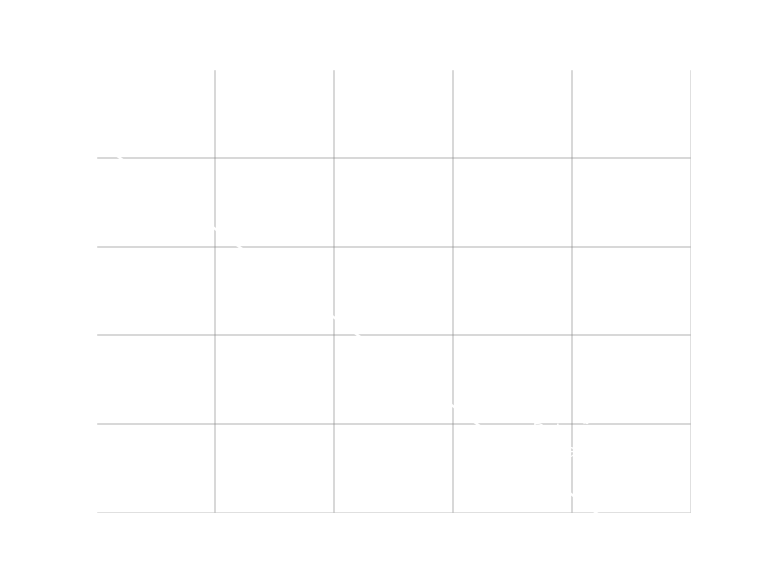
\includegraphics[scale=0.6]{cap32_4-caixa_edgeworth_1.png}}
	\end{figure}

\end{frame}

\begin{frame}
	\frametitle{As Trocas de Mercado}

	\begin{figure}[H]
		\centering
		\colorbox{black}{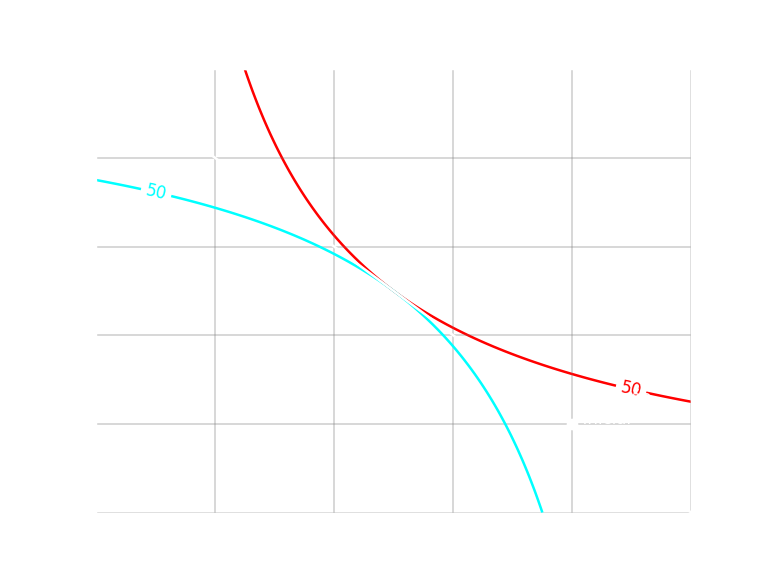
\includegraphics[scale=0.6]{cap32_4-caixa_edgeworth_2.png}}
	\end{figure}
		
\end{frame}

\begin{frame}
	\frametitle{As Trocas de Mercado}

	Vamos recapitular alguns conceitos da teoria do consumidor agora.
	\\~\\
	A \textbf{demanda bruta} é o quanto o consumidor quer consumir de um bem dada sua renda (é obtida pelo cálculo da maximização com restrição lá do capítulo 5). 
	\\~\\
	A \textbf{demanda líquida} ou \textbf{demanda excedente}, é dada pela equação $e_A^1 = x_A^1 - w_A^1$. Se $e_A1 < 0$, ele será um vendedor líquido, caso contrário, ele será um comprador. 
	\\~\\
	A partir de agora, usaremos o termo "demanda"\ para falar da \textbf{demanda bruta} e \textbf{demanda líquida ou excedente} caso queiramos falar desses outros conceitos.

\end{frame}

\begin{frame}
	\frametitle{As Trocas de Mercado}

	Então podemos afirmar que as pessoas sempre serão capazes de chegar a um resultado em trocas uma vez que o leiloeiro defina os preços?
	\\~\\
	A resposta é não
	\\~\\
	É possível que os preços arbitrados não produzam soluções, ou seja, que as escolhas maximizadoras de cada consumidor não sejam compatíveis. Veja um caso onde modificamos os parâmetros da função de utilidade do consumidor A.

\end{frame}

\begin{frame}
	\frametitle{As Trocas de Mercado}

	\begin{figure}[H]
		\centering
		\colorbox{black}{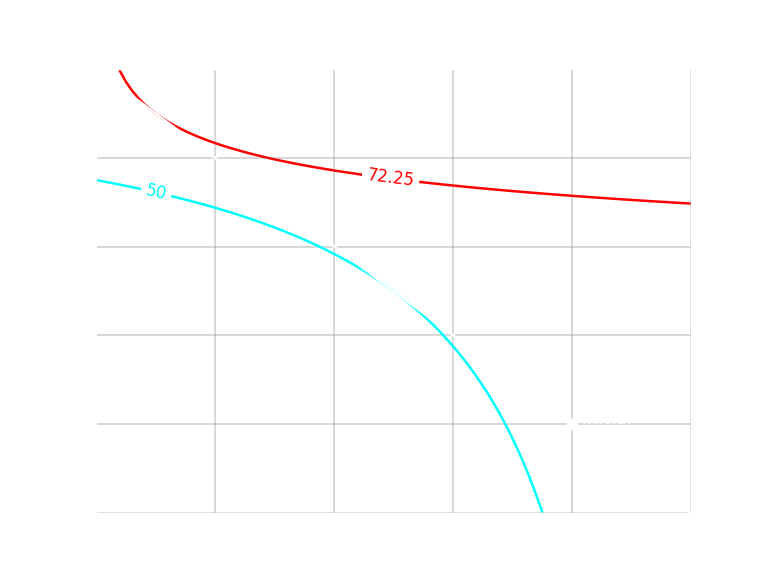
\includegraphics[scale=0.6]{cap32_4-caixa_edgeworth_3.png}}
	\end{figure}
	
\end{frame}

\begin{frame}
	\frametitle{As Trocas de Mercado}

	Nessa situação, os agentes não conseguirão fazer as trocas porque, ao nível de preços dado, eles maximizam em pontos de alocação diferentes. Nós dizemos, nesse casos, que o mercado está em \textbf{desequilíbrio}.
	\\~\\
	Quando o mercado está em desequilíbrio o leiloeiro poderá intervir modificando os preços. 
	\\~\\
	Ele poderá aumentar o preço para os casos de excesso de demanda e reduzir em casos de excesso de oferta (a oferta aqui é quando a demanda líquida é negativa). 

\end{frame}

\begin{frame}
	\frametitle{As Trocas de Mercado}

	\begin{figure}[H]
		\centering
		\colorbox{black}{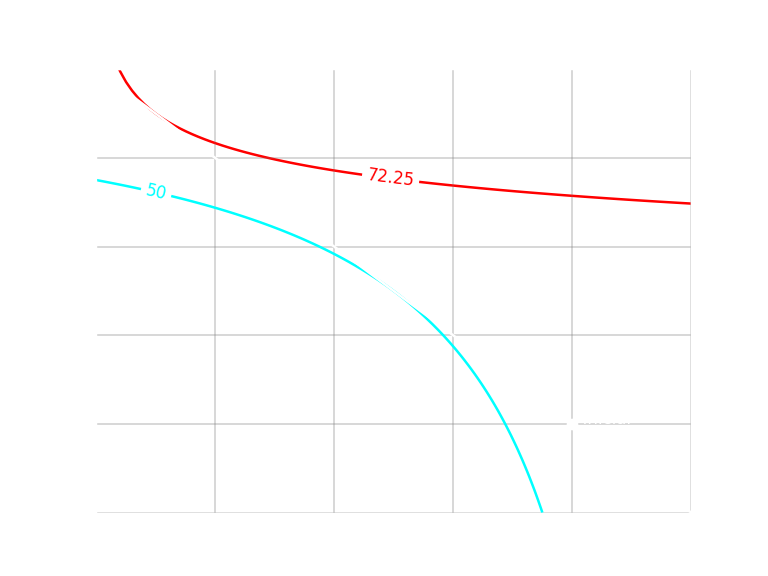
\includegraphics[scale=0.6]{cap32_4-caixa_edgeworth_4.png}}
	\end{figure}
		
\end{frame}

\begin{frame}
	\frametitle{As Trocas de Mercado}

	\begin{figure}[H]
		\centering
		\colorbox{black}{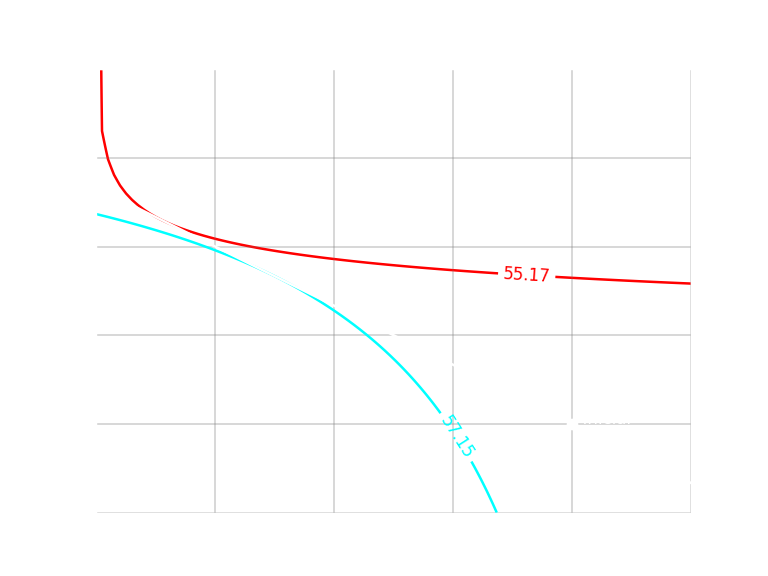
\includegraphics[scale=0.6]{cap32_4-caixa_edgeworth_5.png}}
	\end{figure}

\end{frame}

\begin{frame}
	\frametitle{As Trocas de Mercado}

	\begin{figure}[H]
		\centering
		\colorbox{black}{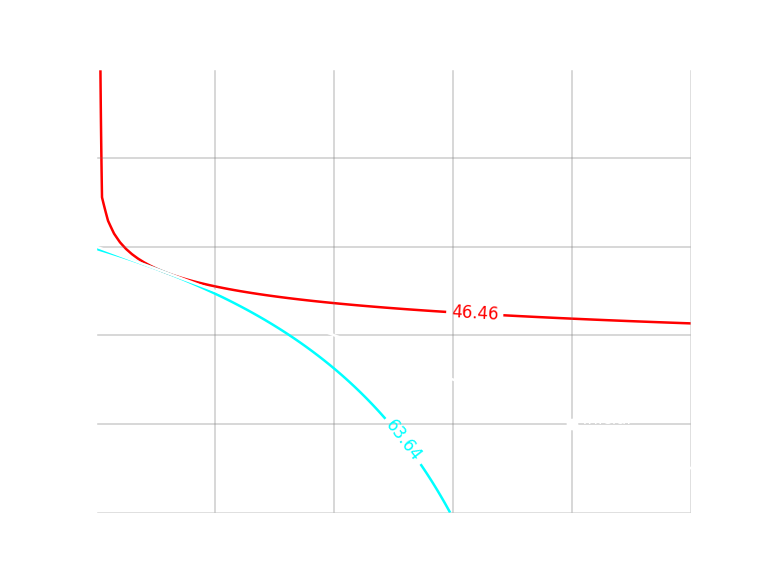
\includegraphics[scale=0.6]{cap32_4-caixa_edgeworth_6.png}}
	\end{figure}

\end{frame}

\begin{frame}
	\frametitle{As Trocas de Mercado}


	O leiloeiro conseguiu uma configuração da alocações onde as demandas são iguais. Nesse ponto, a quantidade total que cada pessoa deseja comprar é igual à quantidade ofertada no mercado. 
	\\~\\
	O mercado está em \textbf{equilíbrio}. 
	\\~\\
	Damos o nome desse tipo de solução em homenagem ao economista francês que primeiro estudou a teoria do equilíbrio geral, Leon Walras. Portanto, chamamos essa alocação de \textbf{equilíbrio walrasiano}\footnote{Outros nomes que esse arranjo recebe são \textbf{equilíbrio de mercado} e \textbf{equilíbrio competitivo}.}.

\end{frame}

\begin{frame}
	\frametitle{A Álgebra do Equilíbrio}

	
	Agora, nos resta construir a solução algébrica desse processo de equilíbrio.
	\\~\\
	Seja $x_A^1(p_1,p_2)$ a função demanda  bem 1 para o agente A e $x_B^1(p_1,p_2)$ a do função demanda do agente B. O equilíbrio walrasiano é obtido pelo par de preços $(p_1^*,p_2^*)$ de modo que

	$$ x_A^1(p_1^*,p_2^*) + x_B^1(p_1^*,p_2^*) = w_A^1 + w_B^1 $$
	$$ x_A^2(p_1^*,p_2^*) + x_B^2(p_1^*,p_2^*) = w_A^2 + w_B^2 $$

	Isso implica que a soma das demandas líquidas seja igual a zero. 
	\\~\\
	No equilíbrio (de duas pessoas), uma pessoa demanda exatamente o que a outra tem interesse em ofertar.

\end{frame}

\begin{frame}
	\frametitle{A Álgebra do Equilíbrio}


	Podemos usar a nossa definição de demandas líquida $e(p_1,p_2) = [x(p_1^*,p_2^*) - w]$ na equação que estamos trabalhando para obtermos

	$$ [x_A^1(p_1^*,p_2^*) - w_A^1] + [x_B^1(p_1^*,p_2^*) - w_B^1] = 0 $$
	$$ [x_A^2(p_1^*,p_2^*) - w_A^2] + [x_B^2(p_1^*,p_2^*) - w_B^2] = 0 $$
	\\~\\
	Ou seja, as somas das demandas líquidas é igual a zero.

\end{frame}

\begin{frame}
	\frametitle{A Álgebra do Equilíbrio}

	Podemos reescrever nosso sistema como

	$$ e_A^1(p_1^*,p_2^*) + e_B^1(p_1^*,p_2^*) = 0 $$
	$$ e_A^2(p_1^*,p_2^*) + e_B^2(p_1^*,p_2^*) = 0 $$
	
	O equilíbrio é obtido pela existência de uma par de preços $(p_1^*,p_2^*)$ cuja demanda excedente agregada seja igual a zero para o bem 1 e para o bem 2.
	\\~\\
	Chamaremos de \textbf{função de demanda excedente agregada} $z(p_1^*,p_2^*)$, a soma das demandas líquidas dos indivíduos para cada par de preços.

\end{frame}

\begin{frame}
	\frametitle{A Álgebra do Equilíbrio}

	$$z_1(p_1^*,p_2^*) = e_A^1(p_1^*,p_2^*) + e_B^1(p_1^*,p_2^*) = 0$$
	$$z_2(p_1^*,p_2^*) = e_A^2(p_1^*,p_2^*) + e_B^2(p_1^*,p_2^*) = 0$$
	\\~\\
	Se a demanda excedente agregada for igual a 0 para o bem 1. Ela sera, necessariamente, igual a 0 para o bem 2. 
	\\~\\
	Para provar essa afirmação nos vamos definir uma propriedade da função de demanda excedente agregada conhecida como \textbf{lei de Walras}.

\end{frame}

\begin{frame}
	\frametitle{A Lei de Walras}

	A lei de Walras afirma que

	$$p_1 z_1(p_1,p_2) + p_2 z_2(p_1,p_2) \equiv 0$$

	Essa é uma \textit{identidade}. Isso quer dizer que temos essa relação para qualquer par de preços, mesmo os que não produzam um equilíbrio.
	\\~\\
	A demonstração decorre do fato que as demandas estão sujeitas as restrições orçamentárias

	$$p_1x_A^1(p_1,p_2) + p_2x_A^2(p_1,p_2) \equiv p_1w_A^1 + p_2w_A^2$$
	$$p_1x_B^1(p_1,p_2) + p_2x_B^2(p_1,p_2) \equiv p_1w_B^1 + p_2w_B^2$$

\end{frame}

\begin{frame}
	\frametitle{A Lei de Walras}

	Trazendo as dotações para o lado esquerdo da equação
	$$p_1[x_A^1(p_1,p_2) - w_A^1] + p_2[x_A^2(p_1,p_2) - w_A^2] \equiv 0$$
	$$p_1[x_B^1(p_1,p_2) - w_B^1] + p_2[x_B^2(p_1,p_2) - w_B^2] \equiv 0$$
	\\~\\
	Reescrevendo usando a notação da demanda excedente
	$$p_1[e_A^1(p_1,p_2)] + p_2[e_A^2(p_1,p_2)] \equiv 0$$
	$$p_1[e_B^1(p_1,p_2)] + p_2[e_B^2(p_1,p_2)] \equiv 0$$

	Essas equações nos dizem que o \textit{valor} (ou seja, preço vezes quantidade do bem 1 + preço vezes quantidade do bem 2) da demanda líquida de cada agente é igual a zero.

\end{frame}

\begin{frame}
	\frametitle{A Lei de Walras}

	Se somarmos as duas identidades, chegaremos a

	$$p_1[e_A^1(p_1,p_2)] + p_2[e_A^2(p_1,p_2)] + 
	p_1[e_B^1(p_1,p_2)] + p_2[e_B^2(p_1,p_2)] \equiv 0$$
	$$p_1[e_A^1(p_1,p_2) + e_B^1(p_1,p_2)] + p_2[e_A^2(p_1,p_2) + e_B^2(p_1,p_2)] \equiv 0$$
	\\~\\
	Veja que os termos dentro dos colchetes são exatamente as funções de demanda excedente agregadas.Ou seja

	$$p_1[z_1(p_1,p_2)] + p_2[z_2(p_1,p_2) ] \equiv 0 \ \blacksquare$$

	Precisamente, a lei de Walras.

\end{frame}

\begin{frame}
	\frametitle{Pausa}

	\begin{figure}[H]
		\centering
		\colorbox{white}{
\includegraphics[scale=0.425]{pausa.png}}
	\end{figure}		

\end{frame}

\begin{frame}
	\frametitle{A lei de Walras}

	Voltemos à nossa afirmação sobre a função de demanda excedente agregada:

	$$z_1(p_1^*,p_2^*) = e_A^1(p_1^*,p_2^*) + e_B^1(p_1^*,p_2^*) = 0$$
	$$z_2(p_1^*,p_2^*) = e_A^2(p_1^*,p_2^*) + e_B^2(p_1^*,p_2^*) = 0$$

	Com a lei de Walras, sabemos que:

	$$p_1 z_1(p_1,p_2) + p_2 z_2(p_1,p_2) \equiv 0$$

	Ou seja, se $z_1(p_1^*,p_2^*) = 0$, pela lei de Walras, será verdade que
	
	$$ 0 + p_2 z_2(p_1,p_2) = 0 $$

	Para qualquer $p_2 \geq 0$ teremos que

	$$z_2(p_1,p_2) = 0$$

\end{frame}

\begin{frame}
	\frametitle{A lei de Walras}

	``Ok, professor. Eu entendi esse argumento todo mas onde a gente vai chegar com tudo isso?''
	\\~\\
	O que acabamos de ver é que, em um mercado de 2 bens e 2 consumidores e dado o par de preços ($p_1^*,p_2^*$), se a função demanda excedente agregada é igual a zero para o bem 1, a função demanda excedente agregada será \textbf{necessariamente} igual a zero para o bem 2.
	\\~\\
	O sinistro é que podemos generalizar esse achado para qualquer quantidade de bens. Em um mercado com $k$ bens e com o vetor de preços ótimos $(p_1^*,p_2^*,...,p_{k-1}^*,p_k^*)$, se as funções demandas excedentes agregadas dos $k-1$ primeiros bens for zero, a função demanda excedente agregada do $k$ bem também será zero.

\end{frame}

\begin{frame}
	\frametitle{Preços Relativos}

	Como podemos encontrar $k$ preços de equilíbrio olhando apenas para $k - 1$ mercados?
	\\~\\
	A verdade é que só existem $k - 1$ preços independentes.
	\\~\\
	Como as relações no modelo de trocas se dão pela equivalência entre as dotações iniciais e as preferências.
	\\~\\
	O que importa entre os preços não é seu \textbf{valor nominal} e sim seu valor \textbf{relativo}. 

\end{frame}

\begin{frame}
	\frametitle{Preços Relativos}

	No exemplo de como o leiloeiro aumentou o preço do bem 2 afim de chegar no equilíbrio do mercado, nós saímos da relação de preço $p_1 = p_2 = 1$ para uma relação $2p_1 = p_2$ (ou seja, $p_2$ é o dobro de $p_1$).
	\\~\\
	Entretanto, nós chegaríamos no mesmo equilíbrio se o leiloeiro \textit{reduzisse} preço do bem 1 para 0,5.
	\\~\\
	Isso nos permite escolher um dos preços como um \textbf{numerário}.
	\\~\\
	Bastando multiplicar todos os $k$ preços por $1/p_k$, chegaremos a um sistema com $k - 1$ preços (que agora estarão dividos por $p_k$) e $k - 1$ equações.

\end{frame}

\begin{frame}
	\frametitle{Preços Relativos}

	A generalização da lei de Walras se configurará em algo como

	$$\frac{p_1}{p_k}z_1(p_1,p_2,...,p_{k-1},1) \ + $$
	$$\frac{p_2}{p_k}z_2(p_1,p_2,...,p_{k-1},1) \ + $$ 
	$$ \vdots $$
	$$\frac{p_{k-1}}{p_k}z_{k - 1}(p_1,p_2,...,p_{k-1},1) \ + $$
	$$z_{k}(p_1,p_2,...,p_{k-1},1) = 0$$
		
	A conclusão é que o modelo de equilíbrio geral é um modelo de equilíbrio de \textbf{preços relativos}.
\end{frame}

\begin{frame}
	\frametitle{A Existência de Equilíbrio}

	A resposta para a pergunta ``Sempre existe um equilíbrio walrasiano para uma economia de trocas qualquer''\ geralmente será não. 
	\\~\\
	Os cientistas trabalharam para responder uma versão um pouco diferente dessa pergunta: ``Sob quais condições, é garantido que exista algum equilíbrio em uma economia de trocas?''.
	\\~\\
	A resposta (versão graduação) para essa pergunta é que a função de demanda excedente deve ser uma \textbf{função contínua}.
	\\~\\
	Uma função é chamada de contínua se \textit{pequenas variações} na suas variáveis independentes resultam em \textit{pequenas variações} variáveis dependentes. Ou seja, não temos \textit{grandes saltos} ou \textit{quebras} no gráfico dessas funções.

\end{frame}

\begin{frame}
	\frametitle{A Existência de Equilíbrio}

	Agora precisamos saber quais são as condições para que a função de demanda excedente seja contínua.
	\\~\\
	No geral, podemos resumir em dois tipos de condições:

	\begin{itemize}
		\item A primeira é que as funções de demanda individuais sejam contínuas (que por sua vez tem como condição que as preferências dos consumidores sejam convexas).
		\item A segunda é que, mesmo que algumas pessoas tenham comportamento descontínuo, se essas forem pequenas em relação ao total do mercado, a função de demanda ainda pode ser contínua (que é um pressuposto bem razoável em se tratando de um mercado competitivo).
	\end{itemize}

\end{frame}

\begin{frame}
	\frametitle{Equilíbrio e Eficiência}

	Como os pontos da curva de contrato são os pontos onde as curvas de utilidade mais altas, ou seja, com maior valor, tangenciam a curva de dotação dos agentes, não há possibilidade de algum deles obter qualquer melhoria preferida pois a escolha de maior utilidade já foi satisfeita dada a restrição orçamentária.
	\\~\\
	Podemos demonstrar essa afirmação de maneira algébrica.
	\\~\\
	Para tal, vamos partir da afirmação oposta ao que queremos provar: ``Vamos partir da hipótese de que o equilíbrio de mercado \textbf{não} é eficiente no sentido de Pareto.''

\end{frame}

\begin{frame}
	\frametitle{A Álgebra da Eficiência}

	Dizer que o equilíbrio de mercado não é eficiente no sentido de Pareto implica na existência de uma alocação possível $(y_A^1,y_A^2,$ $y_B^1,y_B^2)$ de modo que

	$$y_A^1 + y_B^1 = w_A^1 + w_ B^1$$
	$$y_A^2 + y_B^2 = w_A^2 + w_ B^2$$

	onde, se essa alocação y for preferida à outra alocação x será verdade que

	$$(y_A^1 + y_A^2) \succ_A (x_A^1 + x_A^2)$$
	$$(y_B^1 + y_B^2) \succ_B (x_B^1 + x_B^2)$$

	As primeiras equações nos dizem que a alocação y é factível. As segundas relações nos dizem que os agentes A e B preferem a alocação y em detrimento da alocação x.

\end{frame}

\begin{frame}
	\frametitle{A Álgebra da Eficiência}

	Pelo conceito de equilíbrio de mercado, os agentes estão nas alocações que maximizam a sua utilidade dada sua restrição orçamentária.
	\\~\\
	Isso implica em dizer que, se y é preferido ao equilíbrio, essa alocação precisa ser, obrigatoriamente, mais cara que a alocação do equilíbrio, ou seja, está acima da restrição orçamentária de cada agente.
	\\~\\
	Esse argumento pode ser traduzido na forma algébrica

	$$p_1y_A^1 + p_2y_A^2 > p_1w_A^1 + p_2w_A^2$$
	$$p_1y_B^1 + p_2y_B^2 > p_1w_B^1 + p_2w_B^2$$

\end{frame}

\begin{frame}
	\frametitle{A Álgebra da Eficiência}

	Somando as duas inequações, teremos

	$$p_1(y_A^1 + y_B^1) + p_2(y_A^2 + y_B^2) > p_1(w_A^1 + w_ B^1) + p_2(w_A^2 + w_ B^2)$$

	Mas se voltarmos nas duas primeiras equações e substituirmos o lado esquerda dessa inequação, chegaremos ao resultado

	$$p_1(w_A^1 + w_ B^1) + p_2(w_A^2 + w_ B^2) > p_1(w_A^1 + w_ B^1) + p_2(w_A^2 + w_ B^2)$$

	O que é uma contradição, mas isso é exatamente o resultado que queríamos chegar.

\end{frame}

\begin{frame}
	\frametitle{A Álgebra da Eficiência}

	Como derivamos uma contradição partindo da negativa da nossa hipótese, podemos concluir que a hipótese original é verdadeira.
	\\~\\
	Desse modo, podemos afirmar que os equilíbrios de mercado são eficientes no sentido de Pareto.
	\\~\\
	Essa conclusão é tão importante que a comunidade científica denominou como \textbf{Primeiro Teorema da Teoria Econômica do Bem-Estar}.
	\\~\\
	Esse teorema afirma que as alocações obtidas em um mercado competitivo serão eficientes no sentido de Pareto.

\end{frame}

\begin{frame}
	\frametitle{A Álgebra da Eficiência}

	Atente para o fato que o teorema não afirma nada sobre outras características como, por exemplo, a distribuição da renda. A prova disso é que a alocação 100\% para o agente A e 0\% pra o B é eficiente no sentido de Pareto. 
	\\~\\
	O resultado pode até não ser socialmente aceitável ou desejável, mas será necessariamente eficiente.

\end{frame}

\begin{frame}
	\frametitle{Eficiência e Equilíbrio}

	Será possível afirmar que toda alocação eficiente no sentido de Pareto pode ser alcançada por um conjunto de preços definidos por um mercado competitivo? A resposta é sim, mas depende de algumas condições.
	\\~\\
	Um equilíbrio de mercado é o ponto onde as curvas de indiferença dos agentes tangencia a restrição orçamentária em \textbf{um único ponto}.
	\\~\\
	O problema é que um equilíbrio de Pareto não tem nenhuma relação com a restrição orçamentária. Então, sempre que as curvas de indiferença são tangentes, temos um equilíbrio de Pareto.
\end{frame}

\begin{frame}
	\frametitle{Eficiência e Equilíbrio}

	A nossa condição reside justamente na relação entre esses dois conceitos.
	\\~\\
	Se as preferências dos agentes são \textbf{convexas}, para cada equilíbrio de Pareto, haverá alguma lista de preços que possa determinar aquela alocação.
	\\~\\
	Essa condição (de convexidade) das preferências recebeu o nome de \textbf{Segundo Teorema do Bem-Estar}.

\end{frame}

\begin{frame}
	\frametitle{Implicações do 1º Teorema do Bem-Estar}

	Existem alguns pressupostos que fazem parte do teorema que merecem ser explicitados para melhor compreensão:
	\\~\\
	\begin{itemize}
		\item Os agentes só se preocupam com seu consumo de bens e não com a escolha dos demais agentes. Não há \textbf{externalidade no consumo}.

		\item Os agentes agem de maneira competitiva. Nós já vimos que o modelo de dois consumidores é apenas uma ferramenta didática.

		\item O teorema só é relevante em um contexto de equilíbrio competitivo. Se temos poder de mercado esse teorema não se aplicaria.
	\end{itemize}

\end{frame}

\begin{frame}
	\frametitle{Implicações do 1º Teorema do Bem-Estar}

	Esses pressupostos constituem um estrutura poderosa (e também uma delimitação clara) para a utilização do modelo competitivo de alocação.
	\\~\\
	Sempre que tivermos relativa confiança que determinado mercado é competitivo, os consumidores só precisarão saber os preços para alocar suas dotações de maneira eficiente.
	\\~\\
	Essa redução da necessidade de informação para a tomada da decisão de consumo é um forte argumento para adoção desse modelo quando precisamos alocar recursos escassos.

\end{frame}

\begin{frame}
	\frametitle{Implicações do 2º Teorema do Bem-Estar}

	O segundo teorema afirma que, se as preferências são convexas, podemos alcançar qualquer alocação eficiente de Pareto pelo sistema de preços.
	\\~\\
	A implicação poderosa desse teorema é que as discussões de eficiência e distrição da riqueza podem ser separadas. Os preços alocam a renda via mecanismo de escassez relativa. Já a distribuição diz respeito a quantidade que os agentes poderão comprar.
	\\~\\
	Se um determinado contexto é muito desigual na dotação inicial, poderíamos redistribuir parte da dotação de um agente para o outro.

\end{frame}

\begin{frame}
	\frametitle{Implicações do 2º Teorema do Bem-Estar}

	O que o segundo teorema nos afirma é que o equilíbrio alcançado a partir dessa nova dotação é eficiente no sentido de Pareto.
	\\~\\
	Perceba então que, se a sociedade tem como meta a redução de desigualdade entre as pessoas, uma mudança na \textbf{dotação} (e consequentemente na renda) via transferência entre os agentes produziria uma alocação eficiente de Pareto.
	\\~\\
	Do ponto  de vista teórico, a realocação das dotações não produzirá distorções no mercado.

\end{frame}

\begin{frame}
	\frametitle{Implicações do 2º Teorema do Bem-Estar}

	Não é incomum que, em busca de reduzir a desigualdade, as discussões de política econômica defendam uma intervenção nas decisões de preços.
	\\~\\
	Enquanto os impostos baseados na dotação de bens dos consumidores não geram ineficiência, os impostos que dependem das escolhas dos consumidores (baseados no consumo) geram ineficiência.

\end{frame}

%%%%%%%%%%%%%%%%%%%%%%%%%%%%%%%%%%%%%%%%%%%
\section[Produção]{Produção}
%%%%%%%%%%%%%%%%%%%%%%%%%%%%%%%%%%%%%%%%%%%
\begin{frame}
	\huge Produção \normalsize
	\\~\\
	\begin{multicols*}{2}		
		\begin{itemize}
			\item Economia Robinson
			\item Crusoé S.A.
			\item O Problema da Empresa
			\item O Problema de Robinson
			\item Produção e consumo
			\item 1º Teorema do Bem Estar
			\item 2º Teorema do Bem Estar
			\item Possibilidades de Produção
			\item Vantagem Comparativa
			\item Eficiência de Pareto
			\item Naufrágios S.A.
			\item Consumo
			\item Alocação Descentralizada
		\end{itemize}
	\end{multicols*}
\end{frame}

\begin{frame}
	\frametitle{Equilíbrio Geral}

	No modelo anterior nós trabalhamos apenas o processo de trocas a partir de uma dotação inicial dos agentes.
	\\~\\
	Mas se nosso objetivo é simular o comportamento agregado da sociedade, é bem comum supor que devemos, também, nos esforçar para compreender o processo de decisão envolvido na resposta à pergunta \textbf{quanto produzir?}.
	\\~\\
	Nosso modelo será reduzido para darmos enfoque apenas aos grandes traços da teoria:
	\begin{itemize}
		\item Um único consumidor
		\item Uma única empresa
		\item Dois bens
	\end{itemize}

\end{frame}

\begin{frame}
	\frametitle{A Economia de Robinson Crusoé}

	Chamaremos o nosso único agente de Robinson Crusoé. Como existe apenas 1 ser no nosso modelo, ele terá de fazer tudo: Ele produzirá todo o montante de alimento (cocos) e será o único consumidor.
	\\~\\
	Desse modo, ele pode escolher, para cada período de tempo, entre gastar energia coletando cocos ou descansar na praia.
	\\~\\
	Suporemos que a função de produção de cocos tenha rendimentos marginais decrescentes ao longo do tempo trabalhado.
	\\~\\
	O ponto de maximização ocorre na tangência entre a função de produção e a curva de indiferença mais alta.

\end{frame}

\begin{frame}
	\frametitle{A Economia de Robinson Crusoé}

	\begin{figure}[H]
		\centering
		\colorbox{black}{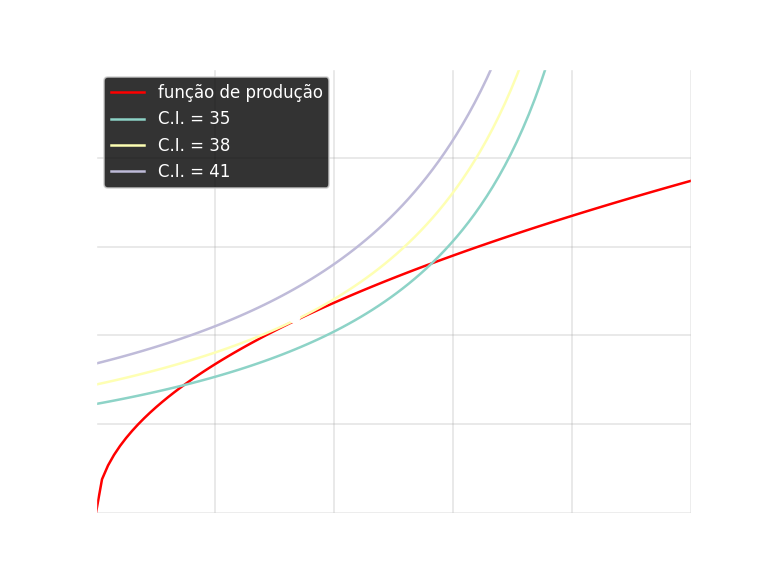
\includegraphics[scale=0.6]{cap33_1-economia_robinson.png}}
	\end{figure}

\end{frame}

\begin{frame}
	\frametitle{Crusoé S.A.}

	Agora vamos viajar pesado na imaginação e criaremos uma empresa dentro desse modelo: a Crusoé S.A. (sim, o Robinson é o único acionista)
	\\~\\
	Ao colocarmos uma empresa maximizadora de lucros dentro do nosso modelo, novas variáveis surgem como, por exemplo, salário, lucro e preço.
	\\~\\
	O objetivo é construir um modelo de equilíbrio geral que seja capaz de igualar, simultaneamente, os preços no mercado de bens e no mercado de trabalho.
	\\~\\
	Definiremos o coco como o nosso numerário. Isso quer dizer que os salários, custos e lucros serão analisados sempre em função da quantidade de cocos. 

\end{frame}

\begin{frame}
	\frametitle{O Problema da Empresa}

	Como toda empresa, a Crusoé S.A. quer maximizar o lucro $\pi$.
	\\~\\
	A receita da empresa será dada pela quantidade de cocos produzida $C$ (já que o coco é o nosso numerário).
	\\~\\
	Para produzir, terá que comprar mão de obra no mercado $L$ e pagar uma quantidade $w$ de salário.
	\\~\\
	De modo algébrico, podemos resumir como:
	$$ \pi = C - wL $$
	$$ C = \pi + wL $$

\end{frame}

\begin{frame}
	\frametitle{O Problema da Empresa}

	Não é difícil ver que essa função função de primeiro grau é uma curva de \textbf{isolucro} lá do capítulo 20.
	\\~\\
	A partir de uma nível inicial de lucro $\pi^*$, a quantidade de cocos que manteria o lucro constante após o pagamento da mão de obra.
	\\~\\
	A maximização nesse caso, ocorre no ponto onde a reta de isolucro intercepta a curva da função de produção.
	\\~\\
	Ponto onde sabemos a quantidade ótima de trabalho $L$ que será adquirida ao custo de $wL$.

\end{frame}

\begin{frame}
	\frametitle{O Problema da Empresa}

	\begin{figure}[H]
		\centering
		\colorbox{black}{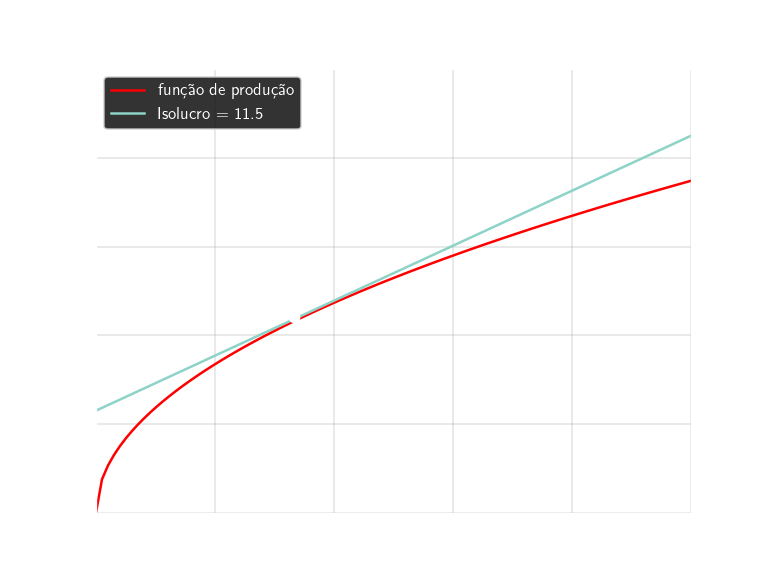
\includegraphics[scale=0.6]{cap33_3-max_lucro.png}}
	\end{figure}

\end{frame}

\begin{frame}
	\frametitle{O Problema de Robinson}

	Após receber seus dividendos, Robinson tem que escolher entre usufruir dos cocos e descansar ou trabalhar na coleta de mais cocos (recebendo seu devido salário).
	\\~\\
	Nós já vimos no capítulo 9 o problema de maximização da utilidade com trabalho.
	\\~\\
	Com esse ponto, conseguimos determinar a oferta de trabalho pela igualdade entre a TMS do consumo pelo lazer e o salário. Exatamente o que vimos no capítulo 9.
	\\~\\	
	Robinson escolherá ofertar a quantidade de trabalho que produza a maior utilidade possível dada sua restrição orçamentária.

\end{frame}

\begin{frame}
	\frametitle{O Problema de Robinson}

	\begin{figure}[H]
		\centering
		\colorbox{black}{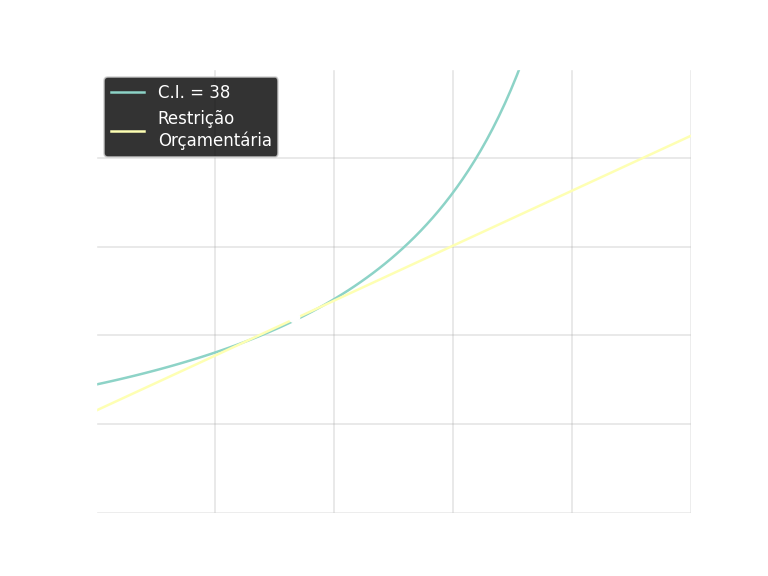
\includegraphics[scale=0.6]{cap33_4-max_trabalho.png}}
	\end{figure}	

\end{frame}

\begin{frame}
	\frametitle{Produção e Consumo}

	Agora que sabemos como Robinson se comportará tanto como acionista da Crosué S.A. e como trabalhador.
	\\~\\
	Podemos colocar esses dois equilíbrios num mesmo gráfico para ver como as variáveis se comportam juntas.
	\\~\\
	Usando nosso instrumento de preços, chegaremos na mesma situação de escolha da primeira seção desse capítulo.
	\\~\\
	Robinson acaba produzindo o ponto cuja produtividade marginal do trabalho\footnote{Que é a inclinação da função de produção.} é igual ao salário.

\end{frame}

\begin{frame}
	\frametitle{Produção e Consumo}

	\begin{figure}[H]
		\centering
		\colorbox{black}{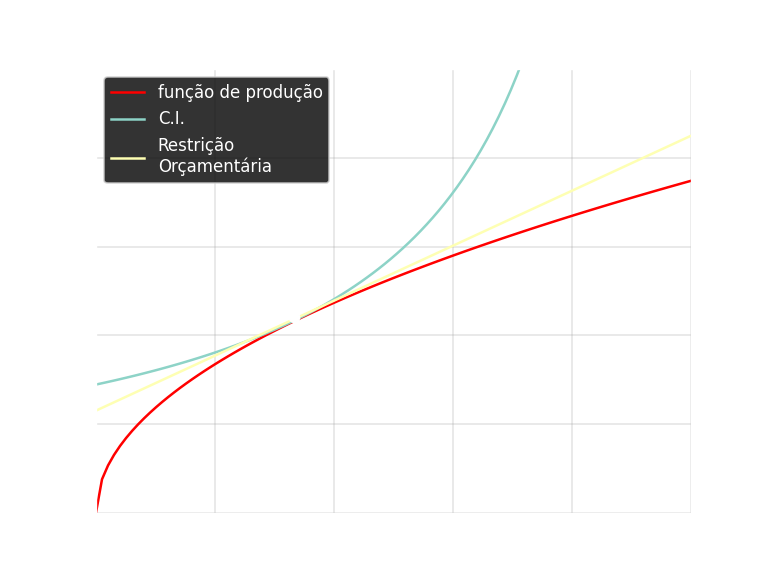
\includegraphics[scale=0.6]{cap33_5-equilibrio.png}}
	\end{figure}

\end{frame}

\begin{frame}
	\frametitle{Produção e Consumo}

	Sim, esse modelo é bem estranho porque sabemos que Robinson decidiria diretamente o que fazer e não ficaria negociando consigo mesmo.
	\\~\\
	Mas isso é apenas uma simplificação didática.
	\\~\\
	Em um cenário com vários atores, os atores agem para maximizar suas preferências a medida que possuem informações sobre o mercado.
	\\~\\
	Os preços são justamente o meio que empresas e trabalhadores recebem as informações para determinar suas ações de modo a maximizar suas escolhas.

\end{frame}

\begin{frame}
	\frametitle{A Produção e o 1º Teorema do Bem-Estar}

	Já sabemos desde a aula passada que as alocações oriundas de uma mercado competitivo são eficientes no sentido de Pareto.
	\\~\\
	O interessante é que essa característica é válida tanto para o equilíbrio oriundo de trocas quanto para o equilíbrio com firmas e consumidores.
	\\~\\
	Não conseguiremos demonstrar essa afirmação acima. Vocês podem conferi-la na página 345 do Microeconomic Analysis.

\end{frame}

\begin{frame}
	\frametitle{A Produção e o 1º Teorema do Bem-Estar}

	As hipóteses de validade do teorema do Bem-Estar para o equilíbrio com produção são parecidas com as do equilíbrio em trocas:
	\\~\\
	\begin{itemize}
		\item Cada empresa maximiza independentemente das outras (\textbf{não existe externalidade na produção}).
		\item Os consumidores são plenamente independentes (\textbf{não existe externalidade no consumo})
		\item A igualdade não é uma característica desenvolvida no modelo. Aqui só olhamos para a \textbf{eficiência}.
	\end{itemize}

\end{frame}

\begin{frame}
	\frametitle{A Produção e o 2º Teorema do Bem-Estar}

	Também já sabemos que toda alocação ótima de Pareto é alcançável por um vetor de preços walrasiano.\footnote{Qual a condição mesmo?}
	\\~\\
	Do mesmo modo, podemos afirmar que esse achado também se mantém para uma economia com firmas e consumidores.
	\\~\\
	A condição adicional é que a \textbf{tecnologia} também deve ser convexa.
	\\~\\
	A demonstração está na página 456 do Microeconomic Analysis.

\end{frame}

\begin{frame}
	\frametitle{Pausa}

	\begin{figure}[H]
		\centering
		\colorbox{white}{
\includegraphics[scale=0.425]{pausa.png}}
	\end{figure}		

\end{frame}

\begin{frame}
	\frametitle{Possibilidades de Produção}

	Nós vamos ver nessa seção como o modelo de Robinson Crusoé pode ser generalizado para mais de um bem.
	\\~\\
	Vamos aumentar para dois bens (porque assim podemos demonstrar os conceitos em um gráfico bidimensional) mas o pensamento é o mesmo para qualquer número arbitrário de bens produzidos e consumidos no mercado.
	\\~\\
	Robinson terá que decidir quanto do seu tempo produtivo será alocado para cada produto.
	\\~\\
	O conjunto de todas as possibilidades de cestas que podem ser produzidas é chamado de \textbf{conjunto de possibilidade de produção}.

\end{frame}

\begin{frame}
	\frametitle{Possibilidades de Produção}

	Não é nada estranho supormos que o comportamento do Robinson será maximizador, por causa disso, a borda desse conjunto nos interessa porque ela mostra as cestas máximas possíveis.
	\\~\\
	De fato, essa borda é tão importante que damos o nome de \textbf{fronteira de possibilidades de produção} para nos referirmos a ela.
	\\~\\
	Qualquer ponto abaixo da borda é um ponto com capacidade ociosa.

\end{frame}

\begin{frame}
	\frametitle{Possibilidades de Produção}

	Supondo que a função de produção de Robinson para peixes seja de 10 quilos por hora trabalhada e a de cocos seja de 20 quilos.
	\\~\\
	Se Robinson tiver, no máximo, disposto a trabalhar 10 horas por dia, nosso modelo de produção pode ser escrito como

	\begin{equation*}
		\begin{split}
			F = 10L_f \\
			C = 20L_c \\
			L_c + L_f = 10
		\end{split}
	\end{equation*}

	Ou seja

	$$\frac{F}{10} + \frac{C}{20} = 10$$

\end{frame}

\begin{frame}
	\frametitle{Possibilidades de Produção}
	
	\begin{figure}[H]
		\centering
		\colorbox{black}{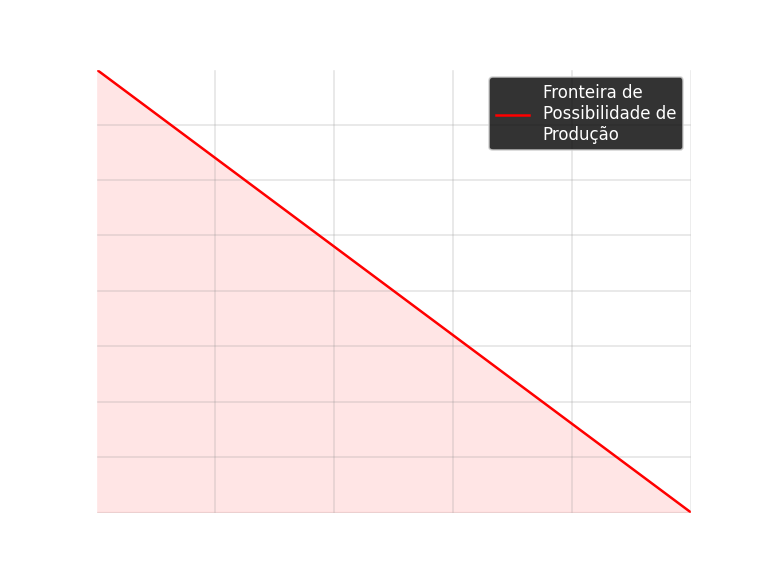
\includegraphics[scale=0.6]{cap33_9-pos_prod1.png}}
	\end{figure}

\end{frame}

\begin{frame}
	\frametitle{Possibilidades de Produção}

	Nós estamos evidenciando o trade-off entre produzir um bem ou outro.
	\\~\\
	Nos gráficos de antes, que tinham as funções de produção, estávamos relacionando os insumos às quantidades produzidas.
	\\~\\
	A inclinação da curva de possibilidade de produção é chamada de \textbf{taxa marginal de transformação}.
	\\~\\
	Ela mostra quanto Robinson precisa abrir mão de um bem para que possa obter mais do outro bem.

\end{frame}

\begin{frame}
	\frametitle{Vantagem Comparativa}

	Se as funções de produção de Sexta-Feira forem diferentes das do Robinson, teremos outra fronteira de possibilidade de produção. Por exemplo, se supormos que as equações forem iguais a 

	\begin{equation*}
		\begin{split}
			F = 20L_f \\
			C = 10L_c \\
			L_c + L_f = 10
		\end{split}
	\end{equation*}

	De modo que

	$$\frac{F}{20} + \frac{C}{10} = 10$$

\end{frame}

\begin{frame}
	\frametitle{Vantagem Comparativa}

	\begin{figure}[H]
		\centering
		\colorbox{black}{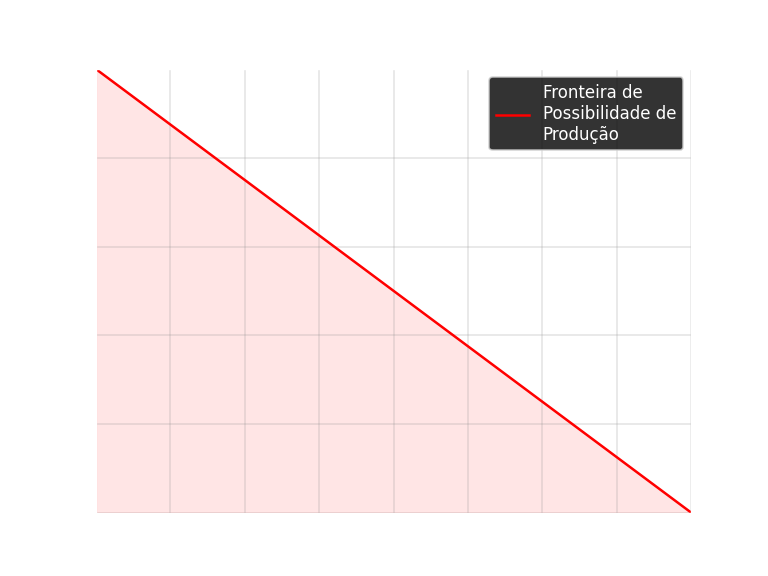
\includegraphics[scale=0.6]{cap33_10-pos_prod1.png}}
	\end{figure}

\end{frame}

\begin{frame}
	\frametitle{Vantagem Comparativa}

	Podemos ver que a taxa de transformação para Robinson é de $\Delta C / \Delta F = -2$ enquanto a taxa de Sexta-Feira é de -1/2.
	\\~\\
	Usamos o termo \textbf{Vantagem Comparativa} para indicar essa diferença entre as taxas de transformação dos produtores.
	\\~\\
	No nosso exemplo, Sexta-Feira tem uma vantagem comparativa na produção de peixe, enquanto Robinson possui uma vantagem comparativa na produção de cocos.

\end{frame}

\begin{frame}
	\frametitle{Vantagem Comparativa}

	Se os dois decidirem agir de maneira conjunta. O máximo de cocos que ambos podem coletar é 300 quilos (sendo 100 de Sexta-Feira e 200 de Robinson).
	\\~\\
	Se eles quiserem algum peixe, faz todo sentido que desloquemos quem possui a vantagem comparativa na produção de peixe.
	\\~\\
	Sexta-Feira trabalhará cada vez mais na produção de peixes até o ponto onde ele produza 200 quilos.
	\\~\\
	A partir desse ponto, teremos que deslocar Robinson para obter mais peixes.

\end{frame}

\begin{frame}
	\frametitle{Vantagem Comparativa}

	\begin{figure}[H]
		\centering
		\colorbox{black}{\includegraphics[scale=0.6]{cap33_10-pos_prod2.png}}
	\end{figure}

\end{frame}

\begin{frame}
	\frametitle{Eficiência de Pareto}

	Podemos retomar o conceito da caixa de Edgeworth para demonstrar como o equilíbrio walrasiano das trocas se comporta junto da produção.
	\\~\\
	Precisamos de um modo que nos permita deduzir como os agentes tomariam suas decisões sobre qual cesta produzir.
	\\~\\
	As cestas ótimas são obtidas pela tangências das curvas de indiferença entre os agentes. Onde as TMS são iguais para ambos os agentes.
	\\~\\
	No nosso modelo atual, a \textbf{quantidade de bens total não é mais fixa} e sim determinada pelos agentes.

\end{frame}

\begin{frame}
	\frametitle{Eficiência de Pareto}

	Para cada alocação ótima das trocas, podemos ter um dos três cenários abaixo:
	\\~\\
	\begin{itemize}
		\item $TMS > TMT$
		\item $TMS < TMT$
		\item $TMS = TMT$
	\end{itemize}

	Os dois primeiros pontos não são, por sí só, eficientes porque os agentes poderiam obter mais de algum bem pela substituição na produção das quantidades.
	\\~\\
	O único ponto onde os agentes estão satisfeitos entre as quantidades produzidas e entre as divisões é o ponto onde as TMS e TMT são iguais.

\end{frame}

\begin{frame}
	\frametitle{Eficiência de Pareto}

	\begin{figure}[H]
		\centering
		\colorbox{black}{\includegraphics[scale=0.6]{cap33_11-edgeworth_prod.png}}
	\end{figure}

\end{frame}

\begin{frame}
	\frametitle{Eficiência de Pareto}

	Vamos observar esse argumento usando cálculo. Primeiro precisamos encontrar uma maneira de descrever a fronteira de possibilidade de produção. A melhor maneira é usando a \textbf{função de transformação}.
	\\~\\
	Essa é uma função das quantidade agregadas dos bens de modo que qualquer combinação $(X^1,X^2)$ estará na fronteira de possibilidade de produção se, e somente se,

	$$ T(X^1,X^2) = 0 $$

	Se colocarmos uma variação positiva de peixe, essa função retornará a variação negativa de coco para que continuemos na fronteira de possibilidade de produção.

\end{frame}

\begin{frame}
	\frametitle{Eficiência de Pareto}

	A taxa marginal de transformação é a inclincação do conjunto de possibilidade de produção, que podemos denotar por $\frac{d X^2}{d X^1}$.
	\\~\\
	Considerando uma pequena mudança na produção $(dX^1,dX^2)$ que ainda seja factível, teremos que

	$$ \frac{\partial T(X^1,X^2)}{\partial X^1} dX^1 + \frac{\partial (X^1,X^2)}{\partial X^2} dX^2 = 0 $$

	Resolvendo para a taxa marginal de transformação

	$$ \frac{d X^2}{d X^1} = - \frac{\partial T/\partial X^1}{\partial T/\partial X^2}  $$

	Vamos segurar essa fórmula para usar mais tarde.

\end{frame}


\begin{frame}
	\frametitle{Eficiência de Pareto}

	Podemos escrever nosso problema de alocação eficiente de Pareto para duas pessoas como

	\begin{center}
		\LARGE $\stackrel{max}{\text{\small $x^1_A,x^2_A,x^1_B,x^2_B$}} \ \ \stackrel{u_A(x^1_A,x^2_A)}{}$ \\
		\normalsize de modo que $u_B(x^1_B,x^2_B) = \overline{u}$ \\
		\normalsize \hphantom{de modo que } $ T(X^1,X^2) = 0 $
	\end{center}

	A Lagrangiana desse problema é

	$$ L = u_A(x^1_A,x^2_A) - \lambda(u_B(x^1_B,x^2_B) - \overline{u}) - \mu(T(X^1,X^2) - 0) $$

\end{frame}

\begin{frame}
	\frametitle{Eficiência de Pareto}

	As condições de primeira ordem são

	$$ \frac{\partial L}{\partial x^1_A} = \frac{\partial u_A}{\partial x^1_A} - \mu\frac{\partial T}{\partial X^1} = 0 $$
	$$ \frac{\partial L}{\partial x^2_A} = \frac{\partial u_A}{\partial x^2_A} - \mu\frac{\partial T}{\partial X^2} = 0 $$
	$$ \frac{\partial L}{\partial x^1_B} = -\lambda\frac{\partial u_B}{\partial x^1_B} - \mu\frac{\partial T}{\partial X^1} = 0 $$
	$$ \frac{\partial L}{\partial x^2_B} = -\lambda\frac{\partial u_B}{\partial x^2_B} - \mu\frac{\partial T}{\partial X^2} = 0 $$

\end{frame}

\begin{frame}
	\frametitle{Eficiência de Pareto}

	Dividindo a primeira equação pela segunda, multiplicando ambos os lados por -1 e rearranjando chegamos a

	$$ - \frac{\partial u_A/\partial x^1_A}{\partial u_A/\partial x^2_A} = - \frac{\partial T/\partial X^1}{\partial T/\partial X^2} $$

	Fazendo a mesma coisa para as equações três e quatro

	$$ - \frac{\partial u_B/\partial x^1_B}{\partial u_B/\partial x^2_B} = - \frac{\partial T/\partial X^1}{\partial T/\partial X^2} $$

\end{frame}

\begin{frame}
	\frametitle{Eficiência de Pareto}

	Olha só que resultado interessante!
	\\~\\
	No lado esquerdo das duas equações finais temos exatamente as taxas marginais de substituição de cada agente. No lado direito, temos aquela relação entre a função de transformação e a taxa marginal de transformação.
	\\~\\
	Podemos ver então que, para o equilíbrio de Pareto, as TMS de cada agente são iguais entre si e, simultaneamente, esse valor da TMS é igual ao valor da TMT.
	\\~\\
	O problema é que essa condição só se refere à \textbf{inclinação} das TMS e TMT e não nos acrescente muito sobre qual será a alocação final além do fato de que ela estará na curva de contrato.

\end{frame}

\begin{frame}
	\frametitle{Náufragos S.A.}

	Nós vamos revisitar o problema da Robinson S.A. mas agora com os dois sócios e trabalhadores: Robinson e Sexta-Feira. Essa nova empresa se chama Naufrágios S.A.
	\\~\\
	Com a expansão do nosso modelo para dois indivíduos, nós temos que descrever o processo de alocação de 4 bens: dois fatores de produção (o quanto de trabalho será contratado de Robinson e Sexta-Feira) e dois produtos (Cocos e Peixes).
	\\~\\
	Agora, a empresa gerará lucros para Robinson e para Sexta-Feira, ou seja, eles precisam decidir, ao mesmo tempo, quanto ofertar de trabalho (de modo a maximizar suas utilidades) e quanto contratar de trabalho (de modo a  maximizar seus lucros).	

\end{frame}

\begin{frame}
	\frametitle{Náufragos S.A.}

	O problema de maximização pode ser descrito como:

	\begin{center}
		\LARGE $\stackrel{max}{\text{\small $C,F,L_F,L_C$}} \ \ \stackrel{p_C C + p_F F - w_C L_C - w_F L_F}{}$
	\end{center}

	Onde C é a produção de cocos, F é a produção de peixes, $L_c$ é a quantidade de trabalho de Robinson e $L_F$ a de Sexta-Feira, $w_C$ é o salário de Robinson e $w_F$ é o de Sexta-Feira e, por fim, $p_C$ e $p_F$ são os preços de mercado.
	\\~\\
	A quantidade total produzida está restrita à fronteira de possibilidade de produção (que nada mais é do que o reflexo das restrições tecnológicas).

\end{frame}

\begin{frame}
	\frametitle{Náufragos S.A.}

	Podemos definir que, no ponto de maximização, a empresa contratará uma quantidade ótima de trabalho $L^*$ de modo que os custos de trabalho podem ser descritos como $L^* = w_C L^*_C + w_F L^*_F$. Podemos reescrever nossa função objeto como:

	$$ \pi = p_C C + p_F F - L^* $$

	Podemos rearranjar a equação para encontrar a solução da quantidade de Cocos

	$$ C = \frac{\pi + L^*}{p_C} - \frac{p_F}{p_C}F $$

\end{frame}

\begin{frame}
	\frametitle{Náufragos S.A.}

	Essa equação descreve as \textbf{retas de isolucro} da empresa.
	\\~\\
	É fácil ver que a inclinação dessas retas será igual à $-p_F/p_C$ e que o os seus interceptos serão iguais a $(\pi + L^*)/p_C$.
	\\~\\
	O problema de maximização do lucro da empresa passa a ser resolvido pela igualdade entre a inclinação da reta de isolucro mais alta e da fronteira de possibilidade de produção. $ TMT = -\frac{p_F}{p_C} $

\end{frame}

\begin{frame}
	\frametitle{Náufragos S.A.}

	\begin{figure}[H]
		\centering
		\colorbox{black}{\includegraphics[scale=0.6]{cap33_12-max_lucros.png}}
	\end{figure}

\end{frame}

\begin{frame}
	\frametitle{Robinson e Sexta-Feira como Consumidores}

	Nós vimos também que o equilíbrio precisa ser em ambos os mercados: produção e consumo. Acabamos de aprender a condição para o lado da produção e agora vamos pensar a respeito do consumo e venda de mão de obra.
	\\~\\
	A renda vem da demanda líquida das dotações dos agentes. Isso é tão verdade, que é simplesmente a expansão da lei de Walras do capítulo 32.
	\\~\\
	Para comprar bens, eles terão que reduzir suas dotações iniciais de lazer (abrindo mão do lazer, trabalharão).
	\\~\\
	Já derivamos a condição que a TMS de ambos os agentes devem ser, necessariamente, igual à TMT. E acabamos de ver que a empresa optará pelo ponto onde a reta de isolucro tangencia a fronteira de possibilidade de produção.

\end{frame}

\begin{frame}
	\frametitle{Robinson e Sexta-Feira como Consumidores}

	\begin{figure}[H]
		\centering
		\includegraphics[scale=0.6]{cap33_13-equilibrio_geral.png}
	\end{figure}

\end{frame}

\begin{frame}
	\frametitle{Conclusão}

	A primeira coisa que podemos ver é que, como Adam Smith desconfiava, é possível derivar um modelo de maximização das utilidades individuais que produza uma alocação ótima dos recursos escassos.
	\\~\\
	Desse modo, podemos resolver problemas sociais intrincados usando esse mecanismo de alocação da escassez relativa dos recursos para que os agentes decidam qual a melhor alocação social.
	\\~\\
	Similarmente, as empresas, buscando a maximização dos seus lucros, também acabam por demandar e remunerar os insumos de modo que, em um modelo fechado, sempre haverá consumo possível.

\end{frame}

%%%%%%%%%%%%%%%%%%%%%%%%%%%%%%%%%%%%%%%%%%%
\section[Bem-Estar]{Bem-Estar}
%%%%%%%%%%%%%%%%%%%%%%%%%%%%%%%%%%%%%%%%%%%
\begin{frame}
	\huge Bem-Estar \normalsize
	\\~\\
	\begin{itemize}
		\item Agregação de Preferências
		\item Funções de Bem-Estar Social
		\item Maximização do Bem-Estar
		\item Funções de Bem-Estar Social Individualistas
		\item Alocações Justas
		\item Inveja e Equidade
	\end{itemize}
\end{frame}

\begin{frame}
	\frametitle{O Bem-Estar}

	No capítulo anterior nós vimos que as alocações ótimas no sentido de Pareto não dizem respeito à distribuição da renda.
	\\~\\
	Já que sabemos que sempre haverá mais de uma alocação eficiente, como escolher qual delas é a melhor?
	\\~\\
	Vamos trabalhar com o conceito da \textbf{função de bem-estar} que permite agregar as utilidades de diferentes consumidores.


\end{frame}

\begin{frame}
	\frametitle{Agregação de Preferências}

	Vamos expandir nossa análise para investigar como a alocação de bens entre os consumidores do mercado pode ser agregada de modo a maximizar o conjunto de preferências ao invés de preferências individuais.
	\\~\\
	Usaremos \textbf{x} para denotar alguma alocação factível.
	\\~\\
	Dadas as alocações \textbf{x} e \textbf{y}, cada pessoa i (ou i-ésima pessoa) será capaz de dizer qual das duas alocações é preferida.
	\\~\\
	Queremos construir uma forma que agregue todas as preferências individuais para construção de uma \textbf{preferências social} que reflita as escolhas individuais.

\end{frame}

\begin{frame}
	\frametitle{Agregação de Preferências}

	Poderíamos pegar as alocações possíveis e perguntar para cada pessoa do mercado: "Você prefere \textbf{x} ou \textbf{y}?" e depois: "Você prefere \textbf{y} ou \textbf{z}?" e assim sucessivamente para todas as alocações desejadas.
	\\~\\
	Terminada essa etapa, poderíamos elencar as cestas preferidas pelo voto da maioria, ou seja, se a maioria das pessoas preferir a alocação \textbf{x} à \textbf{y}, nossa função de utilidade social também representará esse comportamento.
	\\~\\
	Então é isso? Terminamos? A resposta é não. Esse método pode gerar classificações não transitivas.

\end{frame}

\begin{frame}
	\frametitle{Agregação de Preferências}

	A agregação por voto majoritário pode produzir preferências não transitivas, e sem transitividade, não podemos garantir que existam pontos de otimização entre as alocações.
	\\~\\
	Uma outra maneira de tentar agregar as preferências é pela adoção de um sistema de votação com escala ordinal.
	\\~\\
	Nesse modelo, as pessoas atribuem pontos para cada cesta (1 para a mais preferida, 2 para a segunda e etc).
	\\~\\
	No final, podemos somar todos os pontos atribuídos e classificar as opções de acordo com os valores (nesse caso, quanto menor a soma, mais preferida é a alocação).

\end{frame}

\begin{frame}
	\frametitle{Agregação de Preferências}

	Então é isso? Terminamos? A resposta também é não. O problema dessa abordagem é que o resultado pode ser manipulado pela introdução de novas opções.
	\\~\\
	Imagine que um comitê quer que o resultado seja a alocação \textbf{x} mas percebe que, com 5 alternativas, as pessoas vão acabar preferindo outra cesta.
	\\~\\
	Esse comitê pode começar a colocar novas opções que sejam levemente parecidas entre si, de modo a "dividir"\ a base de votantes das alocações preferidas à \textbf{x} anteriormente.
	\\~\\
	Isso vai fazer com que a base de votantes das cestas vencedoras se dilua e a alocação \textbf{x} poderá ser eleita como a vencedora.

\end{frame}

\begin{frame}
	\frametitle{Agregação de Preferências}

	Vamos elencar algumas características desejadas para o nosso mecanismo de decisão social precisa ter:
	\\~\\
	\begin{enumerate}
		\item Dado um conjunto completo, reflexivo e transitivo de preferências individuais, a agregação dessas preferências deve possuir as mesmas propriedades.
		\item Se todas as pessoas preferirem \textbf{x} a \textbf{y}, então, a preferência social deve classificar \textbf{x} à frente de \textbf{y}.
		\item Dadas duas alocações \textbf{x} e \textbf{y}, a preferências social deve depender apenas das escolhas individuais sobre as cestas e não deve ser influenciada pelo modo de classificação das alternativas.
	\end{enumerate}

\end{frame}

\begin{frame}
	\frametitle{Agregação de Preferências}

	Faz sentido querer que nossa agregação de preferências tenham todas as características. O problema é que o trabalho de 1963 de Kenneth Arrow chegou em um resultado surpreendentemente.
	\\~\\
	\textbf{Teorema da Impossibilidade de Arrow}: Se um mecanismo de decisão social satisfizer as propriedades 1, 2 e 3, ele será, necessariamente, uma ditadura: todas as ordenações sociais são ordenações de um único indivíduo.
	\\~\\
	Como esse curso é básico, não vamos demonstrar esse teorema. Se abandonarmos a propriedade 3, alguns tipos de votação ordinal mantém as outras propriedades ativas.

\end{frame}

\begin{frame}
	\frametitle{Funções de Bem-Estar Sociais}

	Sejam as preferências de cada pessoa $i$ relacionadas às alocações possíveis, as funções de utilidade $u_i(x)$ resumem os valores dos julgamentos das pessoas de modo que, a pessoa $i$ prefere \textbf{x} a \textbf{y} se, e somente se, $u_i(x) > u_i(y)$.
	\\~\\
	Apesar da não importância cardinal das funções de utilidade, podemos optar pela construção da nossa função de utilidade social pela soma das utilidades individuais. Desse modo, \textbf{x} é preferido a \textbf{y} se

	$$  \displaystyle \sum^n_{i = 1} u_i(x) > \sum^n_{i = 1} u_i(y)$$

	Sendo $n$ a quantidade de pessoas da sociedade.

\end{frame}

\begin{frame}
	\frametitle{Funções de Bem-Estar Sociais}

	Isso faz sentido mas é totalmente arbitrário. Não existe pressuposto teórico para a definição da função de utilidade social desse modo. Poderíamos usar qualquer outra forma de agregação.
	\\~\\
	Podemos refinar essa ideia com um pressuposto adicional: A nossa função de agregação sempre será crescente na utilidade para cada indivíduo.
	\\~\\
	Isso garante que, se todos preferirem \textbf{x} a \textbf{y} as nossas preferências sociais também escolherão a mesma ordem.

\end{frame}

\begin{frame}
	\frametitle{Funções de Bem-Estar Sociais}

	Essas funções de agregação de preferências individuais recebem o nome de \textbf{função de bem-estar social}.
	\\~\\
	Esse termo denota uma função que é construida tendo como parâmetros as funções de utilidades dos indivíduos da sociedade: $W(u_1(x),u_2(x),...,u_n(x))$.
	\\~\\
	Essa classe de funções nos permite atribuir uma classificação para diferentes alocações tendo com base as utilidades individuais, e, como pressuposto, são crescentes em relação à quantidade de indivíduos.

\end{frame}

\begin{frame}
	\frametitle{Funções de Bem-Estar Sociais}

	Essa função que vimos no slide anterior também recebe o nome de função de bem-estar \textbf{utilitarista clássica} ou de \textbf{Bentham}.

	$$ W(u_1(x),u_2(x),...,u_n(x)) = \displaystyle \sum^n_{i = 1} u_i(x)$$

	Uma generalização dessa função é a \textbf{função de bem-estar da soma ponderada das utilidades}:

	$$ W(u_1(x),u_2(x),...,u_n(x)) = \displaystyle \sum^n_{i = 1} a_iu_i(x)$$

	Onde os pesos $a_i$ são números indicativos da importância de cada agente no total da utilidade geral. Naturalmente, $a$ costuma ser um número positivo.

\end{frame}

\begin{frame}
	\frametitle{Funções de Bem-Estar Sociais}

	Uma outra forma de função de bem-estar interessante é a \textbf{minimax} ou \textbf{rawlsiana}:

	$$ W(u_1(x),u_2(x),...,u_n(x)) = min\{ u_1, u_2, ..., u_n \} $$

	Essa função de bem-estar classifica a alocação pela utilidade da pessoa em pior situação.
	\\~\\
	Todas essas formas podem ser usadas para expressar o que estamos desejando. A única restrição imposta é que a função seja crescente na utilidade de cada consumidor.

\end{frame}

\begin{frame}
	\frametitle{Maximização do Bem-Estar}

	De posse de uma função de bem-estar, podemos começar a trabalhor o problema da maximização.
	\\~\\
	Vamos usar $x_i^j$ para denotar o quanto a pessoa $i$ tem do bem $j$. Na nossa sociedade, existirão $n$ pessoas e $k$ bens.
	\\~\\
	Desse modo, uma dada alocação \textbf{x} será uma lista da quantidade de que cada um dos $n$ agentes possuem dos $k$ bens disponíveis.
	\\~\\
	A quantidade total de cada um dos $k$ bens será dada como fixa, de modo que o total do bem 1 será denotado por $X^1$. A quantidade total disponível do bem 2 será $X^2$ e assim por diante.

\end{frame}

\begin{frame}
	\frametitle{Maximização do Bem-Estar}

	Podemos então definir nosso problema de maximização como:

	\begin{center}
		$\textrm{max } W(u_1(x),u_2(x),...,u_n(x))$ \\
		$\textrm{de modo que } \displaystyle \sum^n_{i = 1} x^1_i = X^1$ \\
		$\textrm{\hphantom{de modo que }} \vdots$ \\
		$\textrm{\hphantom{de modo que }}\displaystyle \sum^n_{i = 1} x^k_i = X^k$
	\end{center}
	
	A alocação possível que maximiza a função de bem-estar deve ter as seguintes características:
	\begin{itemize}
		\item Ela será uma alocação eficiente no sentido de Pareto.
		\item Qualquer alocação eficiente no sentido de Pareto será um ponto de máximo para alguma função de bem-estar.
	\end{itemize}

\end{frame}

\begin{frame}
	\frametitle{Maximização do Bem-Estar}

	Se existir um ponto de máximo e esse ponto não for uma alocação de Pareto, isso implicaria que o ponto ótimo de Pareto daria, pelo menos, o mesmo nível de utilidade que essa alocação hipotética.
	\\~\\
	Como a função de bem-estar tem a propriedade de ser estritamente crescente, ao mudar de alocação para uma alocação de Pareto, para pelo menos uma pessoa, haveria um incremento de utilidade.
	\\~\\
	O que por sua vez, demonstra que a alocação ótima tem de ser uma alocação eficiente de Pareto.

\end{frame}

\begin{frame}
	\frametitle{Maximização do Bem-Estar}

	Chamaremos de \textbf{conjunto de possibilidades de utilidade}, o total de todas as utilidades obtidas da função de bem-estar para diferentes alocações.
	\\~\\
	A curva na borda desse conjunto recebe o nome de \textbf{fronteira de possibilidades de utilidade} e indica os pontos de alocação que permitem o valor máximo para a função de bem-estar social.
	\\~\\
	As curvas de isobem-estar são as curvas que demonstram um mesmo nível de bem estar para ambos os agentes.
	\\~\\
	Como previsto pela primeira propriedade, o ponto máximo é um ponto em que a curva de possibilidade de utilidade tangencia a curva de isobem-estar mais elevada.

\end{frame}

\begin{frame}
	\frametitle{Maximização do Bem-Estar}

	\begin{figure}[H]
		\centering
		\includegraphics[scale=0.55]{cap34_3-maximizacao_bem_estar.png}
	\end{figure}

\end{frame}

\begin{frame}
	\frametitle{Maximização do Bem-Estar}

	A segunda propriedade é fruto da convexidade do conjunto de possibilidade de utilidade.
	\\~\\
	Como o conjunto é convexo, sempre podemos definir uma função de bem-estar que seja tangente à esse conjunto em algum ponto dele.
	\\~\\
	Desse modo podemos ver que a função de bem-estar nos dá uma forma de escolher alocações eficientes no sentido de Pareto pois todo máximo de bem-estar é um ótimo de Pareto e todo ótimo de Pareto será o máximo de alguma função de bem-estar.

\end{frame}

\begin{frame}
	\frametitle{Funções de Bem-Estar Social Individualistas}

	As funções de bem-estar que usamos até agora são compostas pelas funções de utilidade de cada agente.
	\\~\\
	Contudo, essas funções de utilidade estão sendo aplicadas à alocação total em vez de uma cesta específica. Isso é uma limitação que podemos retirar do modelo.
	\\~\\
	Para permitir que os indivíduos se preocupem apenas com as suas próprias cestas, vamos adicionar um índice $i$ a cada cesta da nossa função de bem-estar. Desse modo, substituiremos $u_i(x)$ por $u_i(x_i)$.
	\\~\\
	Isso significa que a utilidade de cada pessoa será referente a sua própria cesta de bens.

\end{frame}

\begin{frame}
	\frametitle{Funções de Bem-Estar Social Individualistas}

	Nossa função de bem-estar terá a forma

	$$ W(u_1(x_1),u_2(x_2),...,u_n(x_n)) $$
	
	Essa nova função de bem-estar será uma função direta em relação aos níveis de utilidade de cada pessoa e indireta em relação às cestas de consumo.
	\\~\\
	O nome dado a essa forma é \textbf{função de bem-estar individualista} ou \textbf{função de bem-estar de Bergson-Samuelson}.
	\\~\\
	Se a utilidade de cada agente não levar em conta nada além da sua própria cesta, dizemos que não há externalidade de consumo.
	\\~\\
	O que nos trás os resultados obtidos no modelo de equilíbrio geral: Os teoremas do Bem-Estar.

\end{frame}

\begin{frame}
	\frametitle{Funções de Bem-Estar Social Individualistas}

	Uma vez que existe essa relação entre a eficiência de Pareto e a maximização do bem-estar, podemos concluir que todo máximo de bem-estar são equilíbrios competitivos e todos os equilíbrios competitivos são o máximo de bem-estar de alguma função de bem-estar.
	\begin{center}
		$$ \underset{x_A^1,x_A^2,x_B^1,x_B^2}{max} \ \ W(u_A(x_A^1,x_A^2),u_B(x_B^1,x_B^2)) $$
		\\
		\normalsize de modo que $T(X^1,X^2) = 0$
	\end{center}

	Onde $X^1$ e $X^2$ denotam o total do bem 1 e 2 produzido e consumido.

\end{frame}

\begin{frame}
	\frametitle{Funções de Bem-Estar Social Individualistas}

	A Lagrangiana desse problema é dada por

	$$ L = W(u_A(x_A^1,x_A^2),u_B(x_B^1,x_B^2)) - \lambda(T(X^1,X^2) - 0) $$

	As condições de maximização são obtidas pelas seguintes condições de primeira ordem:
	\small
	$$ \frac{\partial L}{\partial x_A^1} = \frac{\partial W}{\partial u_A} \frac{\partial u_A(x_A^1,x_A^2)}{\partial x_A^1} - \lambda \frac{\partial T(X^1,X^2)}{\partial X^1} = 0 $$

	$$ \frac{\partial L}{\partial x_A^2} = \frac{\partial W}{\partial u_A} \frac{\partial u_A(x_A^1,x_A^2)}{\partial x_A^2} - \lambda \frac{\partial T(X^1,X^2)}{\partial X^2} = 0 $$

	$$ \frac{\partial L}{\partial x_B^1} = \frac{\partial W}{\partial u_B} \frac{\partial u_B(x_B^1,x_B^2)}{\partial x_B^1} - \lambda \frac{\partial T(X^1,X^2)}{\partial X^1} = 0 $$

	$$ \frac{\partial L}{\partial x_B^2} = \frac{\partial W}{\partial u_B} \frac{\partial u_B(x_B^1,x_B^2)}{\partial x_B^1} - \lambda \frac{\partial T(X^1,X^2)}{\partial X^2} = 0 $$
	\normalsize
\end{frame}

\begin{frame}
	\frametitle{Funções de Bem-Estar Social Individualistas}

	Fazendo exatamente o que vimos no capítulo anterior, chegaremos numa situação onde teremos:

	$$ - \frac{\partial u_A / \partial x_A^1}{\partial u_A / \partial x_A^2} = - \frac{\partial T / \partial X^1}{\partial T / \partial X^2} $$
	$$ - \frac{\partial u_A / \partial x_B^1}{\partial u_A / \partial x_B^2} = - \frac{\partial T / \partial X^1}{\partial T / \partial X^2} $$
	
	Podemos ver que a maximização da função de bem-estar nos dá as condições de primeira ordem que nos certificam uma alocação eficiente no sentido de Pareto.

\end{frame}

\begin{frame}
	\frametitle{Alocações Justas}

	A nossa teoria de função de bem-estar pode ser boa para descrever a utilidade do agregado social mas podemos usar outras abordagens para trazer alguns julgamentos éticos a esse problema.
	\\~\\
	Uma abordagem, chamada de \textbf{estudo das alocações justas}, tenta analisar os pontos de equilíbrio a apartir de alguns julgamentos morais específicos e suas implicações.
	\\~\\
	Se dividirmos $n$ bens igualmente entre três pessoas, A, B e C. Supondo que A e C possuam as mesmas preferências.	

\end{frame}

\begin{frame}
	\frametitle{Alocações Justas}

	Se você usar o princípio moral da igualdade, as alocações iniciais ideais de cada pessoa serão $n/3$. Como as pessoas são diferentes em preferências, haverá o incentivo de trocas.
	\\~\\
	Se A e B fazem uma troca, teremos um aumento do bem-estar social que nos leva a um ótimo de Pareto. Mas C não teve a chance de trocar com ninguém e, nesse caso, pode \textbf{invejar} a pessoa A.
	\\~\\
	Podemos ver que a simetria nas alocações não é suficiente para preservar a simetria do equilíbrio.
	\\~\\
	O que levanta a questão se é possível, partindo do princípio da equidade, que alguma alocação ótima de Pareto seja garantida a partir de uma alocação.

\end{frame}

\begin{frame}
	\frametitle{Inveja e Equidade}

	Uma locação será \textbf{equitativa} se nenhum agente prefere a cesta de bens de outro agente em relação à sua própria cesta. Caso contrário, se a pessoa $i$ preferir a cesta da pessoa $j$ diremos que $i$ \textbf{inveja} $j$. Se uma alocação for, simultaneamente, equitativa e eficiente no sentido de Pareto, ela será chamada de uma alocação \textbf{justa}.
	\\~\\
	Com essa formalização, podemos ver que uma alocação inicial simétrica, possui a propriedade de ser equitativa, contudo, não é a única alocação em que essa propriedade possa ser encontrada.
	\\~\\
	Para verificarmos que uma alocação justa possa existir, vamos voltar ao exemplo da seção anterior (que é uma dotação inicial equitativa), mas agora vamos usar o mecanismo de mercado para encontrar uma alocação final.
	

\end{frame}

\begin{frame}
	\frametitle{Inveja e Equidade}

	Já sabemos pelo capítulo 32 que o resultado será uma alocação em que cada agente maximiza a cesta via preços $(p_1,p_2)$. Sabemos também que esse resultado será eficiente no sentido de Pareto.
	\\~\\
	Mas seria essa alocação equitativa? Para descobrirmos, vamos supor o contrário. Suporemos que A inveja B. Isso significa que a cesta de B é preferida por A da seguinte forma:
	
	$$ (x_A^1,x_A^2) \prec_A (x_B^1,x_B^2) $$
	
	O termo $\prec_A$ denota a preferência do consumidor A.
	\\~\\
	Acontece que, se A prefere a cesta de B ao invés da sua. E, ao mesmo tempo, a cesta de A é resultante de trocas.

\end{frame}

\begin{frame}
	\frametitle{Inveja e Equidade}

	Isso implica que A não pode, aos preços $(p_1,p_2)$, pagar pela cesta de B, ou seja:

	$$ p_1w_A^1 + p_2w_A^2 < p_1w_B^1 + p_2w_B^2 $$
	
	Mas isso é impossível! Afinal, nós partimos de uma alocação inicial equitativa. Isso resulta que a nossa afirmação inicial que A prefere a cesta de B é falsa.
	\\~\\
	Portanto, a alocação inicial equitativa resulta, pelo mecanismo de mercado competitivo, em uma alocação final justa.
	\\~\\
	Na imagem a seguir vamos comparar duas alocações hipotéticas. Uma é resultante de uma troca por qualquer outro mecanismo e a alocação justa é resultante da troca por mecanismo de mercado.

\end{frame}

\begin{frame}
	\frametitle{Inveja e Equidade}

	\begin{figure}[H]
		\centering
		\includegraphics[scale=0.55]{cap34_6-inveja_equidade.png}
	\end{figure}

\end{frame}

%%%%%%%%%%%%%%%%%%%%%%%%%%%%%%%%%%%%%%%%%%%
\section[Externalidades]{Externalidades}
%%%%%%%%%%%%%%%%%%%%%%%%%%%%%%%%%%%%%%%%%%%
\begin{frame}
	\huge Externalidades \normalsize
	\\~\\
	\begin{itemize}
		\item Fumantes e Não Fumantes
		\item Preferências Quase Lineares e Teorema de Coase
		\item Produção de Externalidades
		\item Interpretação das Condições
		\item Sinais de Mercado
		\item A Tragédia dos Comuns
	\end{itemize}
\end{frame}


\begin{frame}
	\frametitle{Externalidades}

	Sempre que um consumidor se preocupar com a produção ou o consumo de outro agente, dizemos que há uma \textbf{externalidade de consumo}. Ela pode ser \textbf{negativa} ou \textbf{positiva}.
	\\~\\
	Sempre que uma atividade produtiva gerar efeitos que influenciem a tomada de decisão dos agentes, diremos que existe uma \textbf{externalidade na produção}. Pode ser \textbf{negativa} ou \textbf{positiva}.
	\\~\\
	Uma externalidade nada mais é do que um bem (ou serviço) que a pessoa se preocupa (ou seja, possui alguma utilidade positiva ou negativa) e que não é comercializado no mercado.
	\\~\\
	É justamente a falta desses mercados para as externalidades que causa o aparecimento de problemas econômicos.

\end{frame}

\begin{frame}
	\frametitle{Externalidades}

	Os modelos vistos até agora tinham a hipótese que os agentes se preocupariam apenas com suas preferências e os preços.
	\\~\\
	Agora vamos relaxar essa abordagem e supor que existirão interações entre os agentes sem que o mecanismos de mercado esteja presente.
	\\~\\
	Ao final do capítulo, vamos ver algumas maneiras de minimizar os problemas causados pelas externalidades via instituições que "emulam"\ um mecanismo de mercado.

\end{frame}

\begin{frame}
	\frametitle{Fumantes e Não Fumantes}

	Imagine que temos dois agentes A e B. Esses dois agentes possuem preferências sobre dois bens "dinheiro"\ e "fumaça".
	\\~\\
	Vamos supor que ambos gostam de dinheiro.
	\\~\\
	Além disso, vamos pensar o que aconteceria se A fosse fumante enquanto B gosta de ar puro.
	\\~\\
	Podemos representar o problema desses dois agentes na caixa de Edgeworth

\end{frame}

\begin{frame}
	\frametitle{Fumantes e Não Fumantes}

	\begin{figure}[H]
		\centering
		\includegraphics[scale=0.6]{cap35_1-dinheiro_fumaca.png}
	\end{figure}

\end{frame}

\begin{frame}
	\frametitle{Fumantes e Não Fumantes}

	Vamos testar duas dotações iniciais, mas em ambas, vamos supor que cada um deles terá a mesma quantidade inicial de dinheiro.
	\\~\\
	Na dotação E (que tem fumaça igual a 0), o agente B está disposto a permitir que A fume (e produza fumaça) em troca de algum dinheiro até o ponto onde as curvas de indiferença dos dois sejam tangentes entre si (cesta X).
	\\~\\
	Na dotação E', teremos o mesmo pensamento, mas agora, o agente B é quem pagará para o agente A reduzir a quantidade de fumaça gerada (cesta Y).

\end{frame}

\begin{frame}
	\frametitle{Fumantes e Não Fumantes}

	Podemos ver que o resultado da alocação final é grandemente impactado pela dotação inicial dos agentes.
	\\~\\
	Tanto a cesta X quanto a Y são eficientes no sentido de Pareto mas o resultado eficiente não implica em nada relacionado às consequências distributivas da alocação.
	\\~\\
	Existe todo um conjunto de cestas ótimas no sentido de Pareto (a curva de contrato) que poderia resultar em alguma alocação eficiente.
	\\~\\
	Para saber onde os agentes acabarão na curva de contrato, precisaremos saber dos \textbf{direitos de propriedade} sobre os bens e serviços que serão utilizados no processo de troca.

\end{frame}

\begin{frame}
	\frametitle{Fumantes e Não Fumantes}

	Podemos repensar esse exemplo como o ponto E sendo o direito de B ao ar puro e o ponto E' sendo o direito de A fumar o quanto quiser.
	\\~\\
	Se houver a possibilidade do detentor do direito vendê-lo, o resultado alcançado será ótimo no sentido de Pareto.
	\\~\\
	Isso mesmo, um mercado de fumaça.
	\\~\\
	Desde que haja direitos de propriedade bem definidos com relação ao bem gerador da externalidades, independente de quem esse direito pertença, os agentes podem usar o mecanismo de trocas a partir da dotação para alcançar uma alocação ótima de Pareto.
	\\~\\
	Isso "internaliza"\ a externalidade e acaba com a distorção impeditiva do alcance do equilíbrio ótimo.

\end{frame}

\begin{frame}
	\frametitle{Fumantes e Não Fumantes}

	Podemos citar vários exemplos práticos:
	\begin{itemize}
		\item Direito de não se vacinar x Direito de não ser infectado
		\item Direito de fazer barulho em casa x Direito ao silêncio
		\item Direito de cobrar o máximo dos alunos x Direito de passar de ano
	\end{itemize}

	Qualquer lado nesses dilemas, está fazendo uso dos seus valores e princípios.
	\\~\\
	Mas, do ponto de vista econômico, todos esses conflitos seriam resolvidos se existisse uma linha clara de direitos de propriedade e um mercado associado.

\end{frame}

\begin{frame}
	\frametitle{Preferências Quase Lineares e o Teorema de Coase}

	A alocação de um mercado com externalidade e direitos de propriedade bem definidos dependerá da dotação inicial dos agentes.
	\\~\\
	Contudo, existe um caso especial onde não importa de quem é o direito de propriedade.
	\\~\\
	Se as preferências dos agentes forem \textbf{quase lineares}, todas as curvas de contrato estarão em uma mesma distribuição da externalidade.
	\\~\\
	Nesse caso, a quantidade de fumaça seria a mesma independente de quem é o direito.

\end{frame}

\begin{frame}
	\frametitle{Preferências Quase Lineares e o Teorema de Coase}

	\begin{figure}[H]
		\centering
		\includegraphics[scale=0.6]{cap35_2-teorema_coase.png}
	\end{figure}

\end{frame}

\begin{frame}
	\frametitle{Preferências Quase Lineares e o Teorema de Coase}

	Essa conclusão que em certas circunstâncias a quantidade da externalidade independer dos direitos de distribuição é conhecida como \textbf{Teorema de Coase}.
	\\~\\
	Outra interpretação do trabalho de Coase é a de que se as negociações de externalidades não possuírem custos de transação, elas levariam a um resultado alocativo ótimo de Pareto.
	\\~\\
	Mas perceba que esse é um resultado bem específico e não deve ser generalizado para qualquer cenário.

\end{frame}

\begin{frame}
	\frametitle{Produção de Externalidades}

	Imagine que temos duas empresas em uma mesma cidade, a empresa S produz uma quantidade de aço $s$ e, como consequência da produção, também produz poluição $x$ que é despejada no num rio.
	\\~\\
	A segunda empresa F é de venda de pescados e se localiza no rio abaixo da empresa S. Desse modo a quantidade de poluição de S afeta a produção de F.
	\\~\\
	Podemos definir a função custo da empresa S como $c_s(s,x)$ e da empresa F como $c_f(f,x)$.
	\\~\\
	A quantidade de poluição é parâmetro comum nas duas funções.

\end{frame}

\begin{frame}
	\frametitle{Produção de Externalidades}

	Vamos definir que impacto de $x$ em cada empresa será diferente, de modo que, $\partial c_f/ \partial x > 0$ e $\partial c_s/ \partial x \leq 0$, ou seja, a poluição aumenta o custo da empresa pesqueira mas não afeta (ou até mesmo reduz) o custo da empresa de aço.
	\\~\\
	O problema de maximização da empresa de aço será

	\begin{center}
		\LARGE $ \stackrel{max}{\text{\small $s,x$}} \ \ %enunciado
		\stackrel{p_s s - c_s(s,x)}{\ } $ %funcao maximizada
	\end{center}

	E da empresa pesqueira seria

	\begin{center}
		\LARGE $ \stackrel{max}{\text{\small $f,x$}} \ \ %enunciado
		\stackrel{p_f f - c_f(f,x)}{\ } $ %funcao maximizada
	\end{center}

\end{frame}

\begin{frame}
	\frametitle{Produção de Externalidades}

	Da maneira como as coisas estão, a empresa de pesca terá de esperar a empresa de aço definir sua quantidade de poluição para poder maximizar seu lucro.
	\\~\\
	As condições de maximização do lucro da empresa S serão

	$$ \frac{\partial c_s(s^*,x^*)}{\partial s} = p_s $$
	$$ \frac{\partial c_s(s^*,x^*)}{\partial x} = 0 $$

	e, para empresa F será

	$$ \frac{\partial c_f(f^*,x^*)}{\partial f} = p_f $$
	
\end{frame}

\begin{frame}
	\frametitle{Produção de Externalidades}

	A empresa S optará produzir a quantidade de poluição que produza o menor custo possível enquanto a empresa F terá de tomar a poluição como dada e maximizar seu lucro a partir desse custo exógeno.
	\\~\\
	Como chegaremos em uma arranjo que permita que a empresa de aço produza mais poluição do que deveria?
	\\~\\
	O custo a mais que a empresa de pesca incorre pela poluição é chamado de \textbf{custo social}.
	\\~\\
	O nosso objetivo é compensar a externalidade para alcançar um equilíbrio de Pareto.

\end{frame}

\begin{frame}
	\frametitle{Produção de Externalidades}	

	Podemos supor que as empresas se unam. Agora, existirá apenas uma empresa de aço e pesca.
	\\~\\
	Consequentemente, não existe mais externalidade nesse caso, uma vez que, a empresa agora \textbf{internalizou} os custos oriundos da produção de poluição. O novo probema de maximização do lucro passa a ser

	\begin{center}
		\LARGE $ \stackrel{max}{\text{\small $s,f,x$}} \ \ %enunciado
		\stackrel{p_s s + p_f f - c_f(f,x) - c_s(s,x)}{\ } $ %funcao maximizada
	\end{center}

\end{frame}

\begin{frame}
	\frametitle{Produção de Externalidades}

	Que possui as seguintes condições de maximização

	$$ \frac{\partial c_s(s^*,x^*)}{\partial s} = p_s $$
	$$ \frac{\partial c_f(f^*,x^*)}{\partial f} = p_f $$
	$$ \frac{\partial c_s(s^*,x^*)}{\partial x} + \frac{\partial c_f(f^*,x^*)}{\partial x}= 0 $$

	O último termo nos assegura que a empresa produzirá poluição até um ponto onde o impacto gerado seja igual à vantagem obtida pela produção desse subproduto.

\end{frame}

\begin{frame}
	\frametitle{Produção de Externalidades}

	Agora, a empresa conjunta precisará adotar a seguinte restrição

	$$ \frac{\partial c_s(s^*,x^*)}{\partial x} + \frac{\partial c_f(f^*,x^*)}{\partial x}= 0 $$
	$$\frac{\partial c_f(f^*,x^*)}{\partial x} = - \frac{\partial c_s(s^*,x^*)}{\partial x} $$

	\begin{center}
		ou
	\end{center}

	$$ - CMa_S(s,x) = CMa_F(f,x) $$

\end{frame}

\begin{frame}
	\frametitle{Produção de Externalidades}

	\begin{figure}[H]
		\centering
		\includegraphics[scale=0.6]{cap35_3-producao_externalidade.png}
	\end{figure}

\end{frame}

\begin{frame}
	\frametitle{Produção de Externalidades}

	Como sabemos, $CMa_F(f,x) > 0$ por pressuposto no começo do modelo. Desse modo, a empresa limitará a produção de poluição até o ponto onde $- CMa_S(s,x) > 0$.
	\\~\\
	Quando a empresa foca em reduzir seus custos privados, ela decide produzir uma quantidade de externalidade maior do que o ótimo de Pareto permite. 
	\\~\\
	Desse modo, o problema da maximização para alcance do ótimo de Pareto é a minimização dos custos sociais e não apenas dos custos privados.
	\\~\\
	No ótimo de Pareto, a soma dos custos marginais de poluição das duas empresas é igual a zero.

\end{frame}

\begin{frame}
	\frametitle{Interpretação das Condições}

	A primeira abordagem é supor que a empresa de aço não está se defrontando com o preço correto da poluição.
	\\~\\
	O custo zero pela poluição não é o preço correto pelo problema causado à empresa de pesca.
	\\~\\
	A partir desse ponto de vista, podemos argumentar que deveria haver uma maneira de punir o produtor da externalidade de modo a fazer com que ele pague pela custo social gerado.
	\\~\\
	Uma forma de fazê-lo pagar é pela criação de um imposto associado à poluição da siderúrgica.

\end{frame}

\begin{frame}
	\frametitle{Interpretação das Condições}

	\begin{center}
		\LARGE $ \stackrel{max}{\text{\small $s,t$}} \ \ %enunciado
		\stackrel{p_ss - c_s(s,x) - tx}{\ } $ %funcao maximizada
	\end{center}
	
	As condições de primeira ordem de maximização do lucro são
	
	$$ p_s - \frac{\partial c_s(s,x)}{\partial s} = 0 $$
	$$ - \frac{\partial c_s(s,x)}{\partial x} - t = 0 $$
	
	Podemos ver que
	
	$$ t = - \frac{\partial c_s(s,x)}{\partial x} $$

\end{frame}

\begin{frame}
	\frametitle{Interpretação das Condições}

	Da seção anterior, nós já tínhamos visto que a condição de otimização do custo social é dada pela seguinte relação 

	$$\frac{\partial c_f(f^*,x^*)}{\partial x} = - \frac{\partial c_s(s^*,x^*)}{\partial x} $$

	Ou seja, podemos ver que esse imposto deve ser

	$$ t = - \frac{\partial c_s(s,x)}{\partial x} = \frac{\partial c_f(f^*,x^*)}{\partial x} $$

\end{frame}

\begin{frame}
	\frametitle{Interpretação das Condições}

	Esse tipo de imposto é chamado de \textbf{imposto de Pigou}. E é uma maneira de resolver essa questão da externalidade da produção.
	\\~\\
	Contudo, para se calcular a alíquota deve-se ter conhecimento sobre o nível ótimo de poluição.
	\\~\\
	Se já temos esse dado, podemos simplesmente cobrar da siderúrgica que ela produza somente até o ponto ótimo.

\end{frame}

\begin{frame}
	\frametitle{Interpretação das Condições}

	A outra abordagem é que falta um mercado para poluição.
	\\~\\
	O problema surge porque o produtor possui custo zero para produzir poluição e, do outro lado, a poluição deveria ter um preço negativo, ou seja, alguém deveria receber algo por ela.
	\\~\\
	Se a empresa de pesca tivesse direito a água limpa mas fosse permitido que ela vendesse a permissão de alguma quantidade de poluição. Sendo $q$ o preço pela quantidade de poluição.

\end{frame}

\begin{frame}
	\frametitle{Interpretação das Condições}

	\begin{center}
		\LARGE $ \stackrel{max}{\text{\small $s,x$}} \ \ \stackrel{p_ss - c_s(s,x) - qx}{\ } $ %funcao maximizada
	\end{center}
	
	Enquanto o problema da empresa de pesca seria
	
	\begin{center}
		\LARGE $ \stackrel{max}{\text{\small $f,x$}} \ \ %enunciado 
		\stackrel{p_ff + qx - c_f(f,x)}{\ } $ %funcao maximizada
	\end{center}

	Desse modo, $qx$ entra como custo para a empresa de aço e uma receita para a empresa de pesca.

\end{frame}

\begin{frame}
	\frametitle{Interpretação das Condições}

	 As condições de maximização serão 

	$$ p_s = \frac{\partial c_s(s,x)}{\partial s} $$
	$$ q = - \frac{\partial c_s(s,x)}{\partial x} $$
	$$ p_f = \frac{\partial c_f(s,x)}{\partial f} $$
	$$ q = \frac{\partial c_s(s,x)}{\partial s} $$

\end{frame}

\begin{frame}
	\frametitle{Interpretação das Condições}

	Cada empresa enfrentará o custo marginal social das suas ações.
	\\~\\
	O equilíbrio é encontrado onde o preço pago pela poluição seja igualador para a oferta da permissão de poluição (pela pescadora) e para a demanda da permissão de poluição (pela siderúrgica). Ou seja

	$$-\frac{\partial c_s(s,x)}{\partial x} = \frac{\partial c_s(s,x)}{\partial s}$$

	Esse resultado foi encontrado no exemplo da fusão das duas empresas.

\end{frame}

\begin{frame}
	\frametitle{Interpretação das Condições}

	Mas não precisamos parar por aqui, podemos supor que o direito seja da siderúrgica. Nesse caso, a pescadora terá que negociar (e pagar) pela redução da produção de poluição.
	\\~\\
	O interessante é que o resultado no montante de poluição é o mesmo. Estranho né? Vamos entender o motivo disso agora.
	\\~\\
	Se a siderúrgica possuir o direito em poluir até uma quantidade $\bar{x}$ e a empresa de pesca estiver disposta a negociar.

\end{frame}

\begin{frame}
	\frametitle{Interpretação das Condições}

	Podemos definir o problema como

	\begin{center}
		\LARGE $ \stackrel{max}{\text{\small $s,x$}} \ \ %enunciado 
		\stackrel{p_ss + q(\bar{x} - x) - c_s(s,x)}{\ } $ %funcao maximizada
	\end{center}

	A siderúrgica agora terá duas fontes de receita: vender aço ou vender alívio de poluição. As condições de primeira ordem para o nosso problema são

	$$ p_s - \frac{\partial c_s(s,x)}{\partial s} = 0 $$
	$$ -q - \frac{\partial c_s(s,x)}{\partial x} = 0 $$

\end{frame}

\begin{frame}
	\frametitle{Interpretação das Condições}

	Enquanto o problema da maximização da empresa de pesca será

	\begin{center}
		\LARGE $ \stackrel{max}{\text{\small $f,x$}} \ \ %enunciado 
		\stackrel{p_ff - q(\bar{x} - x) - c_s(f,x)}{\ } $ %funcao maximizada
	\end{center}

	Cujas condições de maximização são

	$$ p_f - \frac{\partial c_f(f,x)}{\partial f} = 0 $$
	$$ q - \frac{\partial c_f(f,x)}{\partial x} = 0 $$

\end{frame}

\begin{frame}
	\frametitle{Interpretação das Condições}

	Essas equações são as mesmas que vimos no caso anterior.
	\\~\\
	Mas agora, quem receberá o recurso será a siderúrgica ao invés da empresa de pesca.
	\\~\\
	Podemos ver que mesmo com o resultado final sendo o mesmo, a questão de quem possui o direito de propriedade é importante para determinar quem deve receber e quem deve pagar pelo custo social.

\end{frame}

\begin{frame}
	\frametitle{Sinais de Mercado}

	A terceira interpretação das externalidades é que o próprio objetivo da maximização dos lucros cria o incentivo à internalização das externalidades.
	\\~\\
	As empresas do nosso exemplo teriam um incentivo em se fundirem de modo a maximizar o lucro coordenado de ambas.
	\\~\\
	Cada dono das empresas poderia vender suas ações pelo valor presente da série de lucros e o comprador, sabendo do ganho oriundo da coordenação das empresas, ganharia pelo fluxo de lucros adicionais oriundo da maximização das atividades.

\end{frame}

\begin{frame}
	\frametitle{Sinais de Mercado}

	Esse comprador poderia ou não ser um dos donos das duas empresas.
	\\~\\
	Com isso, observamos que a própria existência da externalidade pode gerar sua resolução através do incentivo à internalização para maximização dos lucros.
	\\~\\
	Isso implicaria que as externalidades gerariam a próprio remédio em algum grau.

\end{frame}

\begin{frame}
	\frametitle{A tragédia dos Comumns}

	Vamos explorar um caso particularmente famoso chamado de "Tragédia dos comuns".
	\\~\\
	Imagine uma vila agrícola onde cada pessoa cria seu gado em um campo comunitário. Vamos verificar dois cenários: O primeiro onde temos direito de propriedade do campo bem definido e o segundo onde o campo é livre para qualquer morador da vila.
	\\~\\
	O custo da vaca será dado por $a$. A quantidade de leite que cada vaca dá é uma função do número de vacas que pastam junto com ela no campo (quanto mais vacas pastando, menos leite por vaca). $f(c)$ será o valor do leite produzido por $c$ vacas pastando no campo. Desse modo, $f(c)/c$ é o valor médio do leite.

\end{frame}

\begin{frame}
	\frametitle{A tragédia dos Comumns}

	Quantas vacas pastarão na terra se quisermos maximizar a riqueza da vila? O problema de maximização deles pode ser escrito como:

	\begin{center}
		\LARGE $ \stackrel{max}{\text{\small $c$}} \ \ %enunciado 
		\stackrel{f(c) - ac}{\ } $ %funcao maximizada
	\end{center}

	Não é nenhum mistério perceber que a condição de primeira ordem nos dá que $f'(c) = a$ ou seja $PM(c) = a$.
	\\~\\
	Afinal, se o valor do produto marginal for maior que $a$ vale a pena colocar mais uma vaca no pasto, caso contrário, seria melhor vendê-la.

\end{frame}

\begin{frame}
	\frametitle{A tragédia dos Comumns}

	Se o campo fosse privado, esse seria precisamente o resultado. O proprietário do campo só permitiria que houvesse a quantidade de vacas que maximizasse o total de leite.
	\\~\\
	Será que o resultado seria o mesmo com a propriedade comum a todos os moradores?
	\\~\\
	Cada habitante pensaria se vale ou não a pena comprar uma vaca adicional.
	\\~\\
	Se existirem $c$ vacas já pastando no campo, a produção por cabeça será de $f(c)/c$.

\end{frame}

\begin{frame}
	\frametitle{A tragédia dos Comumns}

	O habitante que está pensando em criar uma vaca sabe que a produção passará a ser $f(c+1)$ se ele o fizer.
	\\~\\
	A receita que essa vaca irá gerar para esse morador da vila é de $f(C+1)/(c+1)$.
	\\~\\
	Se $f(C+1)/(c+1) > a$, será lucrativo adicionar uma vaca.
	\\~\\
	Desse modo, os moradores da vila irão produzir até o ponto onde o benefício médio pela vaca adicional for igual ao custo de compra da mesma, ou seja

	$$ \frac{f(\bar{c})}{\bar{c}} = a $$


\end{frame}

\begin{frame}
	\frametitle{A tragédia dos Comumns}

	Isso nada mais é que obedecer à primeira equação do problema de maximização: $f(\bar{c} - a\bar{c} = 0$).
	\\~\\
	Quando uma pessoa pondera em comprar uma vaca, ela pensa apenas no benefício individual que obterá mas, com isso, acaba ignorando que essa vaca adicional reduzirá a quantidade de leite produzido pelas vacas que já estão no pasto.
	\\~\\
	No final, o pasto comunitário terá mais vacas que o ponto de maximização do lucro.

\end{frame}

\begin{frame}
	\frametitle{A tragédia dos Comumns}

	\begin{figure}[H]
		\centering
		\includegraphics[scale=0.6]{cap35_6-tragedia_comum.png}
	\end{figure}

\end{frame}

\begin{frame}
	\frametitle{A tragédia dos Comumns}

	Esse resultado não significa que tudo pode ser resolvido por propriedades privadas e que todo arranjo público será amaldiçoado para o problema do uso comum.
	\\~\\
	O que estamos vendo aqui é que existe a necessidade de se "emular"\ no caso dos bens comuns, alguma restrição que permita que o resultado final seja ótimo.
	\\~\\
	Até porque, nós veremos mais pra frente que existem produtos que não é possível definir claramente a propriedade.

\end{frame}

%%%%%%%%%%%%%%%%%%%%%%%%%%%%%%%%%%%%%%%%%%%
\section[B.Públicos]{Bens Públicos}
%%%%%%%%%%%%%%%%%%%%%%%%%%%%%%%%%%%%%%%%%%%
\begin{frame}
	\huge Bens Públicos \normalsize
	\\~\\
	\begin{multicols*}{2}		
		\begin{itemize}
			\item Quando Prover?
   			\item Provisão Privada
			\item Pegando Carona
			\item Níveis do Bem Público
			\item Preferências Quase Lineares
			\item O Problema do Carona
			\item Comparação com Bens Privados
			\item Votação
			\item Mecanismo Vickrey-Clarke-Groves
			\item Exemplos de VCG
		\end{itemize}
	\end{multicols*}
\end{frame}


\begin{frame}
	\frametitle{Bens Públicos}

	Infelizmente, nem todas as externalidades são facilmente resolvidas. A medida que número de agentes envolvidos aumenta porque as negociações se tornam cada vez mais complexas e de difícil entendimento.
	\\~\\
	\textbf{Bem Público} que são um tipo particular de externalidade de consumo onde toda pessoa é obrigada a consumir a mesma quantidade do bem.
	\\~\\
	Por exemplo, podemos citar a defesa de um país, a poluição atmosférica, os fogos de artifícios na virada do ano.
	\\~\\
	Todos esses bens são distribuídos igualmente mesmo que algumas pessoas percebam seus valores diferentemente.

\end{frame}

\begin{frame}
	\frametitle{Quando Prover um Bem Público?}

	Vamos supor que haja dois colegas de quarto, 1 e 2. Eles estão discutindo para decidir se compram ou não uma televisão.
	\\~\\
	A TV será instalada na sala e poderá ser usufruída por ambos. Desse modo, ela é um bem público ao invés de privado.
	\\~\\
	A pergunta que queremos resolver é: Será que vale a pena para eles comprar essa TV?
	\\~\\
	Seja $w_1$ e $w_2$ a riqueza de cada agente, $g_1$ e $g_2$ são as contribuições de cada um deles para o valor ta TV e $x_1$ $x_2$ é a quantia que sobrará para o restante do consumo de cada um deles.

\end{frame}

\begin{frame}
	\frametitle{Quando Prover um Bem Público?}

	Desse modo, podemos representar as restrições como

	$$ x_1 + g_1 = w_1 $$
	$$ x_2 + g_2 = w_2 $$

	Se o custo da televisão for $c$, então teremos a seguinte relação para que a compra seja possível: $g_1 + g_2 \leq c$.
	\\~\\
	Essa equação é o resumo da tecnologia disponível para oferta desse bem público.

\end{frame}

\begin{frame}
	\frametitle{Quando Prover um Bem Público?}

	A utilidade da pessoa 1 será função do consumo privado $x_1$ e da disponibilidade do bem público (a televisão). Podemos escrever essa função como $u_1(x_1,G)$ onde G é uma variável de controle para a disponibilidade da TV (0 para o cenário sem TV e 1 para o cenário com TV).
	\\~\\
	Similarmente, a utilidade da pessoa 2 pode ser expressa como $u_2(x_2,G)$. Perceba que, diferentemente do consumo privado, a oferta da TV não muda em relação ao agente.
	\\~\\
	Os dois agentes vão avaliar qual o retorno em utilidade obtidos pelo serviço de televisão. Uma medida que podemos usar dessa avaliação pessoal é o \textbf{preço de reserva} de cada um dos agentes.

\end{frame}

\begin{frame}
	\frametitle{Quando Prover um Bem Público?}

	Seja o preço de reserva da pessoa 1 igual a $r_1$. Ao pagar pela TV o seu preço de reserva, lhe restará $w_1 - r_1$ de renda disponível para o resto do seu consumo.
	\\~\\
	Como $r_1$ indica justamente o ponto onde o agente é indiferente ao preço, podemos afirmar que $u_1(w_1 - r_1) = u_1(w_1,0)$.
	\\~\\
	Nesse caso analisado só existem dois pontos eficiêntes no sentido de Pareto. O primeiro é a alocação $(w_1,w_2,0)$ onde não há TV e a utilidade de cada agente virá do seu consumo privado.

\end{frame}

\begin{frame}
	\frametitle{Quando Prover um Bem Público?}

	O outro ponto é a alocação com bem público fornecido, esse ponto $(x_1,x_2,1)$ onde 

	$$ x_1 = w_1 - g_1$$
	$$ x_2 = w_2 - g_2$$
	\ 
	\\~\\
	Quais as condições para o fornecimento da televisão?

\end{frame}

\begin{frame}
	\frametitle{Quando Prover um Bem Público?}

	Bom, só haverá uma melhoria de Pareto se as pessoas estiverem melhor com a TV do que sem ela

	$$u_1(w_1,0) < u_1(x_1,1)$$
	$$u_2(w_2,0) < u_1(x_2,1)$$

	Se aplicarmos a relação do preço de reserva que vimos acima e a restrição orçamentária que acabamos de ver, podemos notar que

	$$u_1(w_1 - r_1,1) = u_1(w_1,0) < u_1(x_1,1) = u_1(w_1 - g_1,1)$$
	$$u_2(w_2 - r_2,1) = u_2(w_2,0) < u_2(x_2,1) = u_2(w_2 - g_2,1)$$

\end{frame}

\begin{frame}
	\frametitle{Quando Prover um Bem Público?}

	Ignorando as igualdades e lembrando que um aumento no consumo implica em aumento da utilidade, teremos

	$$u_1(w_1 - r_1,1) < u_1(w_1 - g_1,1)$$
	$$u_2(w_2 - r_2,1) < u_2(w_2 - g_2,1)$$

	Logo, com uma mesma função de utilidade, só pode ser que

	$$w_1 - r_1 < w_1 - g_1$$
	$$w_2 - r_2 < w_2 - g_2$$

\end{frame}

\begin{frame}
	\frametitle{Quando Prover um Bem Público?}

	O que, por fim, implica em

	$$r_1 > g_1$$
	$$r_2 > g_2$$

	Ou seja, só será melhor para os agentes se o preço pago por cada um deles for menor do que seus respectivos preços de reserva.
	\\~\\
	Também podemos ver que, se o preço de reserva é maior que a parcela de participação da compra, então a soma dos preços de reserva será maior que o custo da TV: $r_1 + r_2 > g_1 + g_2 = c$.

\end{frame}

\begin{frame}
	\frametitle{Quando Prover um Bem Público?}

	É estranho estarmos gastando tanto esforço em um problema relativamente simples. Mas o Varian quer que prestemos atenção em alguns aspectos relevantes desse problema. Os pontos são:
	\begin{itemize}
		\item O bem público só será ofertado se proporcionar uma melhoria de Pareto.
		\item Essa melhoria depende do preço de reserva de cada agente e do custo do bem.
		\item O preço de reserva de cada agente é função da restrição orçamentária de cada agente.
		\item Se a soma dos preços de reservas for maior que o custo do bem, então a oferta do bem público será factível.
	\end{itemize}

\end{frame}

\begin{frame}
	\frametitle{Quando Prover um Bem Público?}

	Vamos verificar esses pontos imaginando que um dos colegas de quarto é louco por TV enquanto o outro quase não liga pra isso.
	\\~\\
	Se o fã de TV tivesse toda a riqueza, ele a compraria porque teria um preço de reserva maior que o custo da mesma.
	\\~\\
	Entretanto, se toda a riqueza estivesse na mão do outro, o fã de TV não teria recurso suficiente para contribuir, de modo que o equilíbrio de Pareto é alcançado pela não oferta da TV.
	\\~\\
	Isso mostra como a distribuição da renda impacta na provisão do bem público.

\end{frame}

\begin{frame}
	\frametitle{Quando Prover um Bem Público?}

	Entretanto, dependendo do formato das preferências, é possível que a oferta do bem público independa da distribuição da renda. Se as preferências forem quase lineares, elas terão a forma

	$$u_1(x_1,G) = x_1 + v_1(G)$$
	$$u_2(x_2,G) = x_2 + v_2(G)$$

	Onde G será 0 ou 1. Se $v_1(0) = v_2(0) = 0$, então a utilidade da não oferta do bem público é igual a zero.
	
\end{frame}

\begin{frame}
	\frametitle{Quando Prover um Bem Público?}
	
	Podemos, então, definir que os preços de reserva serão

	$$u_1(w_1 - r_1,1) = w_1 - r_1 + v_1(1) = u_1(w_1,0) = w_1$$
	$$u_2(w_2 - r_2,1) = w_2 - r_2 + v_1(1) = u_2(w_1,0) = w_2$$

	Podemos ver então, que os preços de reserva serão dados por

	$$r_1 = v_1(1)$$
	$$r_2 = v_2(1)$$

	Nesse caso, desde que $w_1 + w_2 \geq c$ os preços de reserva dependerão apenas da utilidade criada pelo bem público e não da riqueza dos agentes.

\end{frame}

\begin{frame}
	\frametitle{Provisão Privada do Bem Público}

	O fato de termos derivado a condição do preço de reserva de cada agente ser menor que a contribuição não implica que, se essa condição for satisfeita, que sempre haverá a oferta do bem público.
	\\~\\
	Se os agentes decidirem compartilhar a informação dos seus respectivos preços de reserva, não será difícil supor que eles encontrarão uma decisão.
	\\~\\
	Mas também não é incomum acharmos situações onde os agentes não tem incentivo à compartilhar suas informações respectivas ao preço de reserva.

\end{frame}

\begin{frame}
	\frametitle{Provisão Privada do Bem Público}

	Vamos supor que todas as pessoas envolvidas na decisão atribuem o mesmo valor para o bem público e que os preços de reserva individuais fossem maiores que o custo da TV ($r_1 > c$ e $r_2 > c$).
	\\~\\
	A pessoa 1 poderia mentir falando que seu preço de reserva é zero e deixar que a pessoa 2 compre a TV sozinha. Mas a pessoa 2 poderia ter a mesma estratégia.
	\\~\\
	Um bom exemplo é a reunião de condomínio. Todos os condôminos querem melhoras. Mas se pudessem, alegariam que não podem contribuir com as cotas extras e torceriam para que os outros condôminos aceitassem absorver a parte de quem alega não poder pagar.

\end{frame}

\begin{frame}
	\frametitle{Provisão Privada do Bem Público}

	Esse é um caso onde os economistas dizem que as pessoas estão querendo \textbf{pegar carona}.
	\\~\\
	Ou seja, ela quer o benefício do bem público mas não quer pagar por ele.
	\\~\\
	E como o bem é público, não é possível evitar que os caronas usufruam dele uma vez ofertado.
	\\~\\
	Outro exemplo é o do aluno que espera que os outros colegas façam a lista para copiar depois pensa que está pegando carona. Mas essa análise está errada. Porque o produto não é a nota ou o diploma e sim o conhecimento.

\end{frame}

\begin{frame}
	\frametitle{Pegando Carona}

	O problema do carona pode ser modelado usando o nosso aprendizado de teoria dos jogos do capítulo 29.
	\\~\\
	Se cada pessoa tiver disponibilidade de 500 reais para a compra e atribuir o uso da TV o valor de 100 reais. Caso o aparelho custe 150 e a soma dos preços de reserva é maior que o custo da oferta do bem, será eficiente no sentido de Pareto ofertar a televisão. Se uma pessoa apenas decidir comprar, terá um resultado líquido de -50.
	\\~\\
	Vamos supor que não é possível evitar que um colega de quarto tenha acesso à TV, mesmo que ele não tenha pago por ela.

\end{frame}

\begin{lrbox}{\mybox}
\begin{game}{2}{2}[Jogador A][Jogador B]
& $Compra$    & $Nao$ \\
$Compra$  & $-50,-50$   & $-50,100$ \\
$Nao$     & $100,-50$   & $0,0$
\end{game}
\end{lrbox}

\begin{frame}
	\frametitle{Pegando Carona}

	Podemos usar a matriz de ganhos para ver como esse problema se apresenta.

	\begin{center}
		\usebox{\mybox}
	\end{center}

	Esse arranjo pode até lembrar um pouco o dilema do prisioneiro, mas não é o caso.

\end{frame}

\begin{frame}
	\frametitle{Pegando Carona}
	
	No dilema dos prisioneiros, a utilidade era maximizada se eles escolhessem agir coordenadamente fazendo a mesma coisa, nesse caso da TV, a utilidade é maximizada pela escolha de fazer o oposto (se um comprar, o outro vai preferir não comprar).
	\\~\\
	Podemos melhorar essa situação obrigando o jogador B a contribuir pelo menos com uma quantia parcial de 51. 
	\\~\\
	Desse modo, teríamos uma melhoria de Pareto.
	
\end{frame}

\begin{frame}
	\frametitle{Pegando Carona}

	Na verdade, Podemos ver que qualquer pagamento entre 50 e 100 feito ao jogador A seria uma melhoria de Pareto.
	\\~\\
	No geral, é exatamente isso que acontece: as pessoas costumam contribuir com alguma fração do custo do Bem Público.
	\\~\\
	Mas existem arranjos mais complexos (mais agentes ou bens cujo preço de oferta é elevado) que podem produzir resultados não desejados pela sociedade.

\end{frame}

%%%%%%%%%%%%%%%%%%%%%%%%%%%%%%%%%%%%%%%%%%%
\section[I.Assimétrica]{Informação Assimétrica}
%%%%%%%%%%%%%%%%%%%%%%%%%%%%%%%%%%%%%%%%%%%
\begin{frame}
	\huge Capítulo \normalsize
	\\~\\
	\begin{multicols*}{2}		
		\begin{itemize}
			\item 
		\end{itemize}
	\end{multicols*}
\end{frame}


\begin{frame}
	\frametitle{}

	

\end{frame}


\end{document}

